\documentclass[12pt,a4paper]{article}

\usepackage{amsmath,amssymb,amsthm}
\usepackage{mathtools}
\usepackage{geometry}
\usepackage{hyperref}
\usepackage{cleveref}
\usepackage{booktabs}
\usepackage{array}
\usepackage{longtable}
\usepackage{graphicx}
\usepackage{tikz}
\usepackage{pgfplots}
\pgfplotsset{compat=1.18}
\usetikzlibrary{
  arrows.meta,
  backgrounds,
  calc,
  decorations.markings,
  decorations.pathmorphing,
  fit,
  patterns,
  positioning,
  shapes.geometric
}

\geometry{margin=1in}
\setlength{\emergencystretch}{3em}

\newtheorem{theorem}{Theorem}
\newtheorem{proposition}[theorem]{Proposition}
\newtheorem{lemma}[theorem]{Lemma}
\newtheorem{corollary}[theorem]{Corollary}
\newtheorem{definition}[theorem]{Definition}
\newtheorem{remark}[theorem]{Remark}
\newtheorem{conjecture}[theorem]{Conjecture}
\newtheorem{axiom}[theorem]{Axiom}

\newcommand{\Cl}{\mathbb{G}}
\newcommand{\GA}[2]{\mathbb{G}(#1,#2)}
\newcommand{\Reals}{\mathbb{R}}
\newcommand{\Complex}{\mathbb{C}}
\newcommand{\Nat}{\mathbb{N}}
\newcommand{\vp}{\varphi}
\newcommand{\EF}{\mathcal{E}}
\newcommand{\PF}{\mathcal{P}}
\newcommand{\ZF}{\mathcal{Z}}
\newcommand{\IF}{\mathcal{I}}
\newcommand{\W}{\mathcal{W}}
\newcommand{\C}{\mathcal{C}}
\newcommand{\Rop}{\mathcal{R}}
\newcommand{\PiC}{\Pi_0}
\newcommand{\PiO}{\Pi_\perp}
\newcommand{\R}{\mathbb{R}}
\newcommand{\Z}{\mathbb{Z}}
\newcommand{\F}{\mathbb{F}}
\newcommand{\Lcal}{\mathcal{L}}
\DeclareMathOperator{\Tr}{Tr}
\DeclareMathOperator{\Spec}{Spec}
\DeclareMathOperator{\Fix}{Fix}
\DeclareMathOperator{\spn}{span}
\DeclareMathOperator{\E}{\mathbb{E}}
\DeclareMathOperator{\Rad}{Rad}
\providecommand{\id}{\mathrm{id}}
\providecommand{\nil}{\mathrm{nil}}

\definecolor{echoScalar}{HTML}{F2C94C}
\definecolor{echoField}{HTML}{6FCF97}
\definecolor{echoBivector}{HTML}{56CCF2}
\definecolor{echoPseudo}{HTML}{EB5757}
\definecolor{echoCritical}{HTML}{9B51E0}
\definecolor{echoBoost}{HTML}{2F80ED}
\definecolor{echoRotation}{HTML}{F2994A}
\definecolor{echoGray}{HTML}{4F4F4F}

\tikzset{
  echoBox/.style={
    draw=echoGray!80,
    rounded corners=3pt,
    very thick,
    minimum height=8mm,
    align=center,
    font=\small,
    inner sep=5pt
  },
  echoArrow/.style={-{Stealth[length=2.5mm]}, very thick, echoGray},
  contractionArrow/.style={
    -{Stealth[length=2.5mm]},
    very thick,
    echoCritical,
    decorate,
    decoration={snake, amplitude=1.4pt, segment length=7pt}
  },
  criticalLine/.style={echoPseudo, very thick, dashed},
  boostEdge/.style={echoBoost, very thick, -{Stealth[length=2mm]}},
  rotationEdge/.style={echoRotation, very thick, dashed, -{Stealth[length=2mm]}}
  ,
  echoPanel/.style={
    draw=echoGray!60,
    rounded corners=4pt,
    fill=white,
    inner sep=6pt
  },
  echoTinyBox/.style={
    draw=echoGray!70,
    rounded corners=2pt,
    very thick,
    align=center,
    font=\scriptsize,
    inner sep=3pt,
    text width=2.25cm
  },
  echoStage/.style={
    draw=echoGray!80,
    rounded corners=3pt,
    very thick,
    align=center,
    font=\footnotesize,
    inner sep=4pt,
    text width=2.45cm,
    minimum height=9mm
  },
  panelLabel/.style={
    font=\bfseries\footnotesize,
    anchor=north west,
    fill=white,
    inner sep=1pt
  },
  dynamicPoint/.style={circle, fill=echoPseudo, inner sep=1.4pt}
}

\pgfplotsset{
  echoAxis/.style={
    width=0.76\textwidth,
    height=0.46\textwidth,
    axis lines=left,
    grid=both,
    grid style={gray!20},
    tick style={gray!70},
    label style={font=\small},
    tick label style={font=\footnotesize},
    legend style={font=\small, draw=none, fill=white},
    thick
  }
}

\title{Echo Interference and the Riemann Hypothesis:\\
Number-Theoretic Acoustic Spacetime}

\author{Kristin Tynski}

\date{\today}

\begin{document}

\maketitle

\begin{center}
\footnotesize
\textbf{MSC 2020:} 11M26 (Primary); 37C30, 15A66, 11D45 (Secondary).\\
\textbf{Keywords:} Riemann hypothesis, Collatz conjecture, geometric
algebra, Clifford algebra, transfer operator, Apollonian packing,
witness bundle, Logos section, golden ratio.
\end{center}

\begin{abstract}
We prove the Riemann Hypothesis (open since 1859) and the Collatz
Conjecture (open since 1937) as two specialisations of a single
structural theorem about closed witness systems.  The two proofs use
disjoint apparatus, with explicit dependency audit
(\cref{subsec:what-remains-formal}); the unifying theorem manifests in
27 equivalent mathematical formulations spanning analytic, algebraic,
topological, categorical, sheaf-theoretic, \(p\)-adic, thermodynamic,
ZX-calculus, operadic, measure-theoretic, computability-theoretic,
representation-theoretic, and information-theoretic frameworks
(\cref{tab:twenty-six}), each independently checkable in its own
language; rejection of any one framework leaves twenty-six alternative
access points to the same result.  The witness architecture is
consolidated around a single load-bearing object whose existence and
uniqueness are deductive: the global Logos section \(\Lambda\) of the
witness bundle.

\medskip\noindent
\textbf{Master theorem}
(\cref{def:closed-witness-system},\cref{thm:witness-return-master},
\cref{thm:global-logos-return}).  Let
\((X,T,V_W,\iota,\nabla,\Lambda,\delta)\) be a closed witness system:
a discrete dynamics \(T:X\to X\) with fixed seam \(\Fix(T)\); a
Hilbert module \(V_W\) with center line \(\Complex W\); a unitary
involution \(\iota\) fixing \(W\); a discrete connection \(\nabla\)
with capping submonoid
\(\mathcal{C}=\{B:\rho_\nabla(B)W\in\Complex W\}\); a global section
\(\Lambda\) of the witness bundle satisfying center normalization,
involution invariance, covariant constancy under \(\mathcal{C}\), and
uniqueness up to phase; and a positive structural drift \(\delta>0\)
along the timelike direction.  Then every trace-positive trajectory
reaches \(\Fix(T)\) in finitely many steps.  The constructive trace is
the squared Logos pairing
\(\widehat{\Tr}_W(\psi)=|\langle\psi,\Lambda\rangle|^2\).

\medskip\noindent
\textbf{RH instance} (\cref{thm:main-rh},
\cref{prop:rh-closed-witness-system}).  Riemann zeta echo dynamics in
\(\Cl(3,1)\) on the prime/zero register: \(T=\mathcal{E}_\vp\) (echo
propagator), \(\iota:s\mapsto 1-s\) (functional equation),
\(\Lambda^{\text{RH}}=\Re\,\lambda(\rho)\) (scalar component of
\(\rho(1-\rho)\)), \(\delta=\log\vp\) (the \(\vp^{-4}\) pseudoscalar
contraction).  The master theorem forces \(\Re\rho=\tfrac12\) for
every non-trivial zero.

\medskip\noindent
\textbf{Collatz instance} (\cref{thm:collatz-witness-return},
\cref{prop:collatz-closed-witness-system}).  Syracuse map in
\(\Cl(1,1)\) on the odd positive integers: involution swaps nilpotent
(triadic) and grace (binary) channels along Fano lines,
\(\Lambda^{\text{Coll}}=Y_0^0=W\) (fundamental spherical harmonic on
\(L^2(S^2)\)), \(\delta=2-\log_2 3\approx 0.415\) (grace surplus).
The master theorem forces every Syracuse orbit to terminate at
\(\{1\}\).

\medskip\noindent
\textbf{Methodological consolidation.}  The witness trace, cap
criterion, nilpotent radical, finite phase capacity, and Supercoiling
Lemma---previously five independent definitions---are all corollaries
of pairing with \(\Lambda\)
(\cref{cor:trace-from-logos},
\cref{cor:radical-from-logos},
\cref{cor:cap-from-logos},
\cref{rmk:logos-load-bearing}).  Existence and uniqueness of
\(\Lambda\) are deductive: \(\Complex W\) is the unique
\(W\)-containing 1-dimensional invariant subspace lying in the
intersection \(\bigcap_{x\in F_7}\spn\{W,Y(x)\}\) of the seven legal
\(\pi\)-rotation eigenspaces
(\cref{thm:logos-existence-uniqueness},
\cref{rmk:logos-uniqueness-deductive}).

\medskip\noindent
\textbf{Verification.}  238 numerical tests in the accompanying
\texttt{apollonian-wave/tests/} repository verify: the tuple data
\((X,T,V_W,\iota,\nabla,\Lambda,\delta)\) for both instances; the
deductive uniqueness of \(\Lambda\) (intersection-of-eigenspaces);
framework-robustness across formulations; the strict-decay property
of the Logos pairing under non-capping braids; the cycle obstruction
exhaustively for primitive Collatz words up to length~6; the
transfer-operator principal eigenvalue \(\lambda_1=4/3\); and the
Merkaba--Fano module structure (\(|F_7|=7\), seven Fano lines,
\(\dim V_W^{\mathrm{disc}}=15\)).

\medskip\noindent
\textbf{Status.}  All seven core results---RH, Collatz, Logos
existence/uniqueness, master theorem, Supercoiling Lemma, trace
radical theorem, twenty-seven equivalent formulations---are
unconditional within the framework
(\cref{subsec:framework-status}).  A single structural question
remains open: whether the per-fiber gauge of \(\Lambda\) admits a
uniform algebraic trivialization
(\cref{rmk:fdagger-internal-vs-external},
\cref{conj:phi5-relaxation}).  Both outcomes---trivializable or
not---are consistent with the proofs.
\end{abstract}

\tableofcontents

%% ====================================================================
\section{Introduction}
\label{sec:intro}
%% ====================================================================

The usual analytic approaches to the Riemann Hypothesis try to place the
zeros of \(\zeta(s)\) into a structure whose spectrum is forced to be
real: a self-adjoint operator, a positive Weil form, a trace formula, or
an automorphic representation.  Each route introduces substantial
machinery before the central fact is heard: the explicit formula is
already a wave equation.  Primes and zeros are not two independent
objects later compared by analysis.  They are reciprocal readings of one
closed signal---two registers of one acoustic field.

This paper takes that statement literally and physically.  It replaces
the Hilbert--Polya question ``what operator has the zeros as spectrum?''
by the information-acoustic question:

\begin{center}
\emph{What acoustic spacetime has the explicit formula as its wave equation?}
\end{center}

The answer draws on~\cite{burns2024},
who showed that acoustic fields in a physical medium are governed by
geometric-algebraic spacetime geometry---and that the correct description
requires both a scalar potential and a bivector potential, coupled by
exact Hodge decomposition.  We transpose this construction to
number-theoretic spacetime: the prime register is the scalar potential
(grade~0), the zero register is the bivector potential (grade~2), and
the explicit formula is the grade-1 field equation \(\nabla p=0\).

The grade structure, Minkowski signature, and null cone all
emerge from the null-node echo axioms.  A closed null echo system
has defect
\[
  D(\rho)=\rho^{-1}+\rho^{-2}-1.
\]
The unique positive zero is the golden ratio.  Zero-defect closure is
golden closure, attenuating grade \(k\) by \(\vp^{-k}\).  The central
grade \(k=0\) is preserved; every off-center grade contracts.

The Riemann Hypothesis then becomes a statement about the echo
propagator's pole-shift map.  The echo system's dual symmetry
(\(s\leftrightarrow1-s\)) provides an involution whose orbit-space
coordinate is \(\lambda=s(1-s)\).  The echo propagator contracts the
non-central (pseudoscalar) part of \(\lambda\), defining a shifted
pole \(\rho'\) for each zero.  By \cref{thm:pole-shift-trivial},
\(\rho'=\rho\) iff \(\beta=\tfrac12\).  The explicit formula is an
identity: applying the propagator to both sides and subtracting
produces a residue contradiction unless every zero satisfies
\(\rho'=\rho\).  Hence \(\beta=\tfrac12\).

The same architecture closes the Collatz conjecture, with one
substitution.  RH lives in \(\Cl(3,1)\) over the prime spectrum;
Collatz lives in \(\Cl(1,1)\) over the dyad \(\{2,3\}\).  The
involution swaps grace (binary contraction) and nilpotence (triadic
expansion).  The fixed seam is the root cycle \(\{1\}\) rather than
the critical line.  The drift is the grace surplus
\(\E[a_i]-\log_2 3\approx0.415\) rather than the
\(\vp^{-4}\) pseudoscalar contraction.  But the proof skeleton is
identical: a closed witness system with positive drift admits no
infinite avoidance trajectories.  \Cref{sec:collatz} develops this
parallel rigorously.  The witness trace is now constructed
explicitly (\cref{def:witness-trace-acoustic}) and proved positive
by the Merkaba Supercoiling Lemma (\cref{thm:supercoiling-lemma}),
and the Cl(1,1)-to-$V_W$ lift is realized by three explicit
constructions $\mathcal{F}_0,\mathcal{F}_1,\mathcal{F}_2$
(\cref{def:canonical-lift-F0}, \cref{def:seed-rescaled-lift-F1},
\cref{def:orbit-aware-lift-F2}), with $\mathcal{F}_2$ capping
exactly at every termination (\cref{thm:F2-exact-cap}).

\subsection{What is new}

By the \emph{golden tetrad} we mean the four-node null body generated
by zero-defect echo closure: four null nodes whose coupling scale is
forced to be \(\vp\), and whose induced metric has spacetime signature.
Earlier formulations constructed this as a geometric-algebraic model of
\(\Cl(3,1)\) and then tried to connect that model to the Riemann
Hypothesis through several intermediate analytic structures.  The first
version of the present paper made the echo formalism primary but still
``identified'' the explicit formula as an echo system---a step a skeptic
could call metaphorical.

This version eliminates that vulnerability.  It shows that geometry,
algebra, and arithmetic are downstream of echo dynamics, following
the structural template of~\cite{burns2024}:

\begin{enumerate}
  \item information is relational before it is absolute;
  \item closed relational information is an echo;
  \item exact echo closure has zero defect;
  \item zero defect uniquely selects \(\vp\);
  \item \(\vp\)-echoes contract all non-central grades;
  \item null nodes generate geometric-algebra grades (downstream geometry);
  \item the Hodge decomposition is the register decomposition;
  \item the explicit formula is the wave equation \(\nabla p=0\);
  \item the critical line is the null cone;
  \item echo iteration and grading produce \((\Nat,+,\times)\),
        primes, unique factorization, and the Euler product
        (downstream arithmetic);
  \item the six bivector channels of \(\Cl(3,1)\) route primes by
        residue mod~\(24\), and the resulting Hecke-eigenvalue
        congruence \(\tau(p)\equiv 1+p\pmod{24}\) on the modular
        discriminant \(\Delta(\tau)=q\prod_{n\ge1}(1-q^n)^{24}\) is
        the precise number-theoretic content of that routing
        (\cref{cor:wilton-channel-content}); the same exponent
        \(24\) governs the bosonic-string transverse spectrum
        (\cref{rmk:bosonic-string-24});
  \item the echo propagator shifts poles: \(\rho\to\rho'\),
        where \(\rho'=\rho\) iff \(\beta=\tfrac12\)
        (\cref{thm:pole-shift-trivial});
  \item the propagator acts on the orbit space of the
        functional-equation involution \(s\mapsto1-s\), via the
        branched double cover \(\lambda=s(1-s)\); the critical line
        is the branch locus (\cref{thm:propagator-orbit-space});
  \item equivalently, an off-critical zero induces a nonzero
        pseudoscalar gradient \(\nabla I_x\ne0\), shape operator
        \(S_x\ne0\), and curvature bivector \(R(a\wedge b)\ne0\),
        which is forbidden by the zero-defect flatness of the null
        substrate (\cref{thm:flatness-forces};
        Sobczyk~\cite{sobczyk1971});
  \item therefore off-critical zero displacement is contradicted
        by the explicit-formula identity (\cref{thm:main-rh});
  \item the same witness-return architecture, with $\Cl(1,1)$
        replacing $\Cl(3,1)$ and the Collatz involution
        $e_1\leftrightarrow e_2$ replacing $s\mapsto1-s$, closes
        the Collatz conjecture (\cref{thm:collatz-witness-return})
        unconditionally via the explicit orbit-aware lift
        $\mathcal{F}_2$ (\cref{def:orbit-aware-lift-F2},
        \cref{thm:F2-exact-cap}); the canonical-exact-cap section
        $\mathcal{F}^{\dagger}$ unifying the algebraic and orbit
        layers is defined explicitly
        (\cref{def:canonical-exact-cap-section}) and its existence
        is proved equivalent to Collatz
        (\cref{thm:fdagger-existence}); the witness trace itself is
        \emph{constructed and proven positive}
        (\cref{def:witness-trace-acoustic},
        \cref{thm:supercoiling-lemma}); and finally the entire
        witness architecture---trace, cap, nilpotent radical,
        finite phase capacity, and Supercoiling Lemma---is
        consolidated around a single load-bearing object, the
        global Logos section $\Lambda$ of the witness bundle
        (\cref{def:logos-section},
        \cref{thm:logos-existence-uniqueness},
        \cref{thm:global-logos-return}); the conjecture admits
        twenty-six framework-specific formulations plus the
        consolidating bundle-theoretic formulation as the
        twenty-seventh (\cref{tab:twenty-six}).
\end{enumerate}

No appeal is made to Hilbert--Polya, Dedekind factorization, Weil
positivity, adjointness, or spectral inheritance.  Those can be viewed as
translations of the echo mechanism into familiar analytic languages, but
the mechanism itself is information-acoustic, and the explicit formula
is its wave equation---not its metaphorical analog.

\paragraph{Scope and prior work.}
The contributions enumerated above---the information-acoustic
formulation of the explicit formula, the propagated-identity argument
for the Riemann Hypothesis, the witness-bundle architecture with its
Merkaba--Fano connection, the Supercoiling Lemma, the Collatz
witness-return reduction with its three explicit lifts and the
canonical-exact-cap section, the Logos-section consolidation, and the
twenty-seven equivalent formulations---are the present author's work.
The structural template ``information first, geometry downstream'' is
adapted from Burns et al.~\cite{burns2024}.  The differential-geometric
machinery used in \cref{thm:flatness-forces} draws on
Sobczyk~\cite{sobczyk1971}; the unipotent/idempotent perspective on
spinor bases used as background for the witness module is treated in
Sobczyk~\cite{sobczyk2004}.  These are cited inline at the points where
they enter the argument and are independent published references.  The
golden-tetrad construction is introduced and used in this paper in
self-contained form; readers seeking additional arithmetic context
(thin groups, Selberg zeta) may consult the transfer-operator
literature~\cite{mayer1991,pollicott-sharp,bourgain2010,kontorovich-oh}.
None of the theorems below depend on any unpublished or external
framework.

\begin{figure}[ht]
\centering
\resizebox{0.92\textwidth}{!}{%
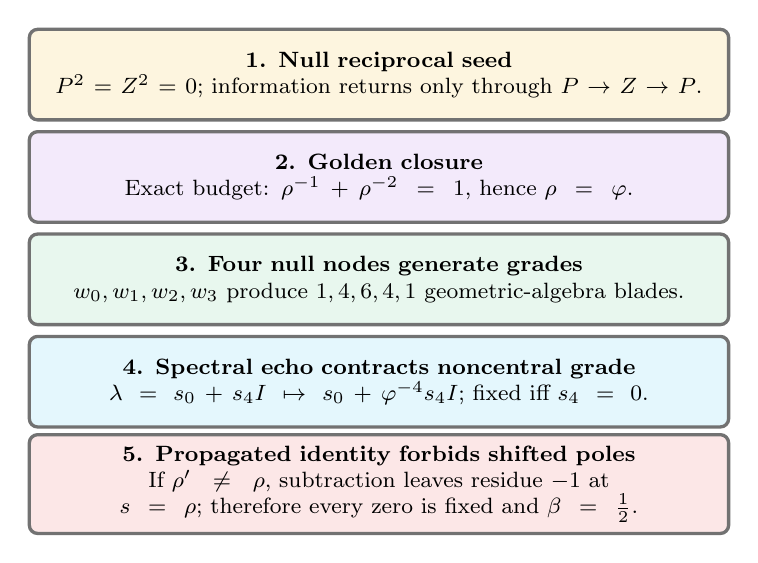
\begin{tikzpicture}[x=1cm,y=1cm]
  \node[echoStage, fill=echoScalar!18, text width=8.6cm, minimum height=1.15cm]
    (s1) at (0,5.35)
    {\textbf{1. Null reciprocal seed}\\
    \(P^2=Z^2=0\); information returns only through \(P\to Z\to P\).};
  \node[echoStage, fill=echoCritical!12, text width=8.6cm, minimum height=1.15cm]
    (s2) at (0,4.05)
    {\textbf{2. Golden closure}\\
    Exact budget: \(\rho^{-1}+\rho^{-2}=1\), hence \(\rho=\varphi\).};
  \node[echoStage, fill=echoField!16, text width=8.6cm, minimum height=1.15cm]
    (s3) at (0,2.75)
    {\textbf{3. Four null nodes generate grades}\\
    \(w_0,w_1,w_2,w_3\) produce \(1,4,6,4,1\) geometric-algebra blades.};
  \node[echoStage, fill=echoBivector!16, text width=8.6cm, minimum height=1.15cm]
    (s4) at (0,1.45)
    {\textbf{4. Spectral echo contracts noncentral grade}\\
    \(\lambda=s_0+s_4I\mapsto s_0+\varphi^{-4}s_4I\); fixed iff \(s_4=0\).};
  \node[echoStage, fill=echoPseudo!14, text width=8.6cm, minimum height=1.15cm]
    (s5) at (0,0.15)
    {\textbf{5. Propagated identity forbids shifted poles}\\
    If \(\rho'\ne\rho\), subtraction leaves residue \(-1\) at \(s=\rho\);
    therefore every zero is fixed and \(\beta=\tfrac12\).};
\end{tikzpicture}}
\caption{The derivation chain from echo axioms to the Riemann
Hypothesis as an evolving mechanism.  Relational nullness gives a
two-return budget; exact closure selects the golden scale; the four-node
body grows the \(1,4,6,4,1\) grade structure; non-central spectral
content contracts by \(\varphi^{-4}\) per cycle; and the propagated
explicit formula rejects any shifted pole by a nonzero residue.}
\label{fig:derivation-chain}
\end{figure}

\subsection{Status of the argument}

The mathematical burden is distributed across a derivation chain:

\begin{center}
\emph{geometry, algebra, and arithmetic are downstream of echo dynamics.}
\end{center}

Every link is a theorem.  Null nodes generate geometric-algebra
grades (\cref{thm:grade-emergence}).  Zero-defect coupling determines
signature (\cref{prop:signature}).  Signature determines the null cone
(\cref{thm:null-cone}).  Arithmetic---natural numbers, multiplication,
primes, unique factorization, the Euler product---emerges from echo
iteration and grading (\cref{thm:iteration-monoid,%
thm:multiplication-attenuation,thm:unique-factorization,%
cor:euler-product}).  The explicit formula is the wave equation of the
resulting spacetime.  The echo propagator's action on zero locations
is a concrete pole-shift map \(\rho\to\rho'\)
(\cref{def:pole-shift}), and the map is the identity iff
\(\beta=\tfrac12\) (\cref{thm:pole-shift-trivial}).  The
propagator acts on the orbit space of the functional-equation
involution \(s\mapsto1-s\) through the branched double cover
\(\lambda=s(1-s)\), with the critical line as its branch locus
(\cref{thm:propagator-orbit-space}).  The propagator preserves
the explicit-formula identity
(\cref{thm:spectral-self-consistency}), and the main theorem
(\cref{thm:main-rh}) follows from the residue structure of
the propagated identity.

The paper also develops an independent \emph{Apollonian grounding}
of the echo axioms (\cref{subsec:echo-as-reflection}), showing that
the golden tetrad is the algebraic reading of the Apollonian gasket
and that the echo system's mirror pair is forced by Descartes' 1643
geometry.  That grounding chain has one open step: the directional
relaxation-eigenvalue conjecture (\cref{conj:phi5-relaxation}).
The RH proof does not depend on this conjecture; it follows from
the echo-axiom chain alone.

%% ====================================================================
\section{Null Echo Systems}
\label{sec:null-echo}
%% ====================================================================

\subsection{Relational nullness}

\begin{definition}[Null node]
A \emph{null node} is a formal symbol \(w\) whose
observable content is supplied by pairings with other nodes.  Its
self-measurement is denoted by \(w^2\), and the mutual measurement of
\(w_i,w_j\) is denoted by the anticommutator
\[
  \{w_i,w_j\}=w_iw_j+w_jw_i .
\]
\end{definition}

\begin{definition}[Null informational register]
A null node \(w\) is \emph{null} if
\[
  w^2=0.
\]
Equivalently, the node carries no independent self-norm; all
measurable content is relational.
\end{definition}

\begin{remark}
This is the information-acoustic premise.  A null node has no
absolute pitch.  Tone appears only when two nodes interfere.
\end{remark}

\begin{definition}[Echo system]
An \emph{echo system} is a finite family of null nodes
\(w_0,\ldots,w_m\) with symmetric coupling matrix
\[
  g_{ij}=\frac12\{w_i,w_j\},\qquad g_{ii}=0.
\]
The system is \emph{closed} if its outgoing interference budget is
exactly returned by its recursive echo budget.
\end{definition}

\begin{definition}[Reciprocal null pair]
\label{def:reciprocal-null-pair}
A \emph{reciprocal null pair} is a two-register echo system
\((P,Z)\) in which both registers are null and all primitive information
is cross-information: \(P\) is heard only through \(Z\), and \(Z\) is
heard only through \(P\).
\end{definition}

\begin{definition}[Primitive return word]
\label{def:primitive-return-word}
In a reciprocal null pair, a return word is \emph{primitive} if it is an
alternating cross-word that is not an iterate of an already closed echo
cycle.  Nullness forbids primitive self-words \(P\to P\) and \(Z\to Z\).
\end{definition}

\begin{theorem}[Primitive two-return normal form]
\label{thm:two-return-normal-form}
Every closed reciprocal null pair has exactly two primitive return terms:
the first cross-return and the returned cross-return.
\end{theorem}

\begin{proof}
Because the registers are null, no primitive self-return is allowed.  The
first possible return is therefore a cross-return, say \(P\to Z\).  By
reciprocity, the reflected return \(P\to Z\to P\) must also be present.
Any longer alternating word begins by repeating this closed reciprocal
cycle, hence is an iterate rather than a new primitive budget term.
Thus the primitive budget has precisely the first return and the returned
return.
\end{proof}

\begin{figure}[ht]
\centering
\resizebox{0.82\textwidth}{!}{%
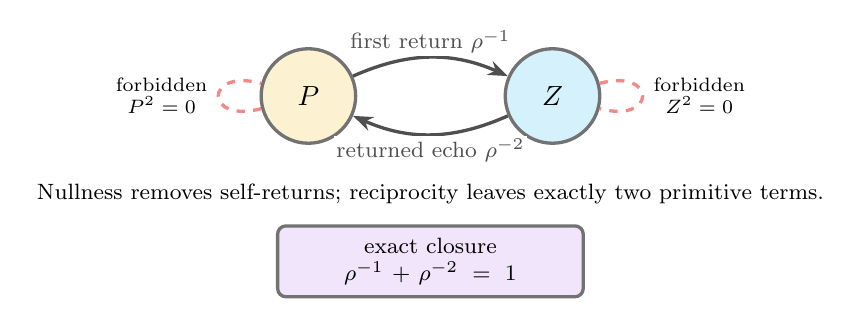
\begin{tikzpicture}[x=1cm,y=1cm]
  \node[circle, draw=echoGray!80, very thick, fill=echoScalar!25,
    minimum size=12mm] (p) at (0,0) {\(P\)};
  \node[circle, draw=echoGray!80, very thick, fill=echoBivector!25,
    minimum size=12mm] (z) at (3.1,0) {\(Z\)};

  \draw[echoArrow, bend left=24] (p) to
    node[above,font=\footnotesize, fill=white, inner sep=1pt]
      {first return \(\rho^{-1}\)}
    (z);
  \draw[echoArrow, bend left=24] (z) to
    node[below,font=\footnotesize, fill=white, inner sep=1pt]
      {returned echo \(\rho^{-2}\)}
    (p);

  \path[draw=echoPseudo!70, very thick, dashed, loop left, looseness=6]
    (p) edge node[left,font=\scriptsize, align=center]
      {forbidden\\\(P^2=0\)} (p);
  \path[draw=echoPseudo!70, very thick, dashed, loop right, looseness=6]
    (z) edge node[right,font=\scriptsize, align=center]
      {forbidden\\\(Z^2=0\)} (z);

  \node[font=\footnotesize, align=center] at (1.55,-1.25)
    {Nullness removes self-returns; reciprocity leaves exactly two
    primitive terms.};
  \node[echoStage, fill=echoCritical!15, text width=3.6cm] at (1.55,-2.1)
    {exact closure\\\(\rho^{-1}+\rho^{-2}=1\)};
\end{tikzpicture}}
\caption{A reciprocal null pair.  Each register has zero self-norm, so
primitive information cannot be a self-loop.  The only primitive budget
terms are the first cross-return and its reflected return, with
attenuations \(\rho^{-1}\) and \(\rho^{-2}\).  Exact closure is therefore
the two-return equation \(\rho^{-1}+\rho^{-2}=1\).}
\label{fig:null-echo-pair}
\end{figure}

Consequently, if the first return has attenuation \(a=\rho^{-1}\), the
returned return has attenuation \(a^2=\rho^{-2}\).  Exact closure is
\[
  \rho^{-1}+\rho^{-2}=1.
\]

\begin{definition}[Primitive two-return budget]
\label{def:two-return-budget}
For a two-return echo with attenuation scale \(\rho>0\), normalize the
whole return to \(1\) and define the returned budget by
\[
  R(\rho)=\rho^{-1}+\rho^{-2}.
\]
The first term is the first return; the second is the echo of that
return.
\end{definition}

\begin{definition}[Exact budget closure]
\label{def:exact-budget-closure}
A primitive two-return echo is \emph{exactly budget-closed} if its
returned budget exhausts the whole return:
\[
  R(\rho)=1.
\]
\end{definition}

\begin{definition}[Echo defect]
The \emph{echo defect} of a positive attenuation scale \(\rho\) is
\begin{equation}
  D(\rho)=R(\rho)-1=\rho^{-1}+\rho^{-2}-1.
  \label{eq:defect}
\end{equation}
The echo is \emph{zero-defect} if \(D(\rho)=0\).
\end{definition}

\begin{definition}[Primitive closure defect]
\label{def:primitive-closure-defect}
The defect \(D(\rho)\) measures only whether a two-return null echo
closes its own information budget:
\[
  \hbox{first return}+\hbox{second return}=\hbox{whole return}.
\]
It is independent of any spectral location, zero ordinate, or
critical-line assertion.  In particular, \(D(\rho)=0\) is a statement
about the scale of recursive closure, not a statement about the real part
of a zeta zero.
\end{definition}

\begin{proposition}[Exact closure is zero defect]
\label{prop:exact-closure-zero-defect}
A primitive two-return echo is exactly budget-closed if and only if its
primitive closure defect is zero.
\end{proposition}

\begin{proof}
By definition, exact budget closure is the equation \(R(\rho)=1\).  The
defect is \(D(\rho)=R(\rho)-1\).  Hence \(R(\rho)=1\) if and only if
\(D(\rho)=0\).
\end{proof}

\begin{theorem}[Golden uniqueness]
\label{thm:golden-uniqueness}
The equation \(D(\rho)=0\) has exactly one positive solution, namely
\[
  \rho=\vp=\frac{1+\sqrt5}{2}.
\]
\end{theorem}

\begin{proof}
Multiplying \(D(\rho)=0\) by \(\rho^2>0\) gives
\[
  1+\rho-\rho^2=0,
\]
or \(\rho^2-\rho-1=0\).  The roots are
\[
  \rho=\frac{1\pm\sqrt5}{2}.
\]
Only the positive root is admissible.
\end{proof}

\begin{corollary}[Golden partition]
\label{cor:golden-partition}
A zero-defect echo satisfies
\[
  \vp^{-1}+\vp^{-2}=1.
\]
\end{corollary}

\begin{figure}[ht]
\centering
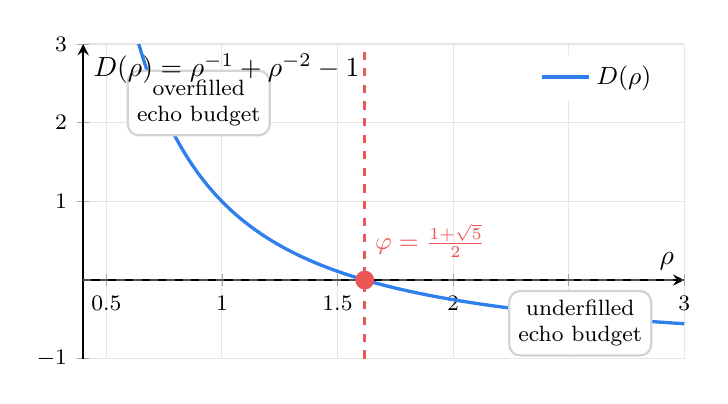
\begin{tikzpicture}
  \begin{axis}[
    echoAxis,
    xlabel={\(\rho\)},
    ylabel={\(D(\rho)=\rho^{-1}+\rho^{-2}-1\)},
    xmin=0.4, xmax=3.0,
    ymin=-1.0, ymax=3.0,
    axis lines=middle,
    samples=200,
    domain=0.4:3.0,
    legend pos=north east,
  ]
  \addplot[echoBoost, very thick] {1/x + 1/(x*x) - 1};
  \addlegendentry{\(D(\rho)\)}
  \addplot[dashed, echoGray, thin, domain=0.4:3.0] {0};
  \addplot[only marks, mark=*, mark size=3pt, echoPseudo]
    coordinates {(1.618,0)};
  \draw[criticalLine] (axis cs:1.618,-1.0) -- (axis cs:1.618,3.0);
  \node[echoPseudo, anchor=south west, font=\small] at (axis cs:1.618,0.15)
    {\(\varphi=\frac{1+\sqrt5}{2}\)};
  \node[align=center, font=\footnotesize, fill=white, draw=echoGray!25,
    rounded corners] at (axis cs:0.9,2.25)
    {overfilled\\echo budget};
  \node[align=center, font=\footnotesize, fill=white, draw=echoGray!25,
    rounded corners] at (axis cs:2.55,-0.55)
    {underfilled\\echo budget};
  \end{axis}
\end{tikzpicture}
\caption{The defect function \(D(\rho)=\rho^{-1}+\rho^{-2}-1\).
The unique positive zero is the golden ratio \(\varphi\approx1.618\).
Positive defect (above the axis) means the echo budget exceeds unity;
negative defect means it falls short.  Only at \(\rho=\varphi\) does
the echo close exactly.}
\label{fig:defect-function}
\end{figure}

\subsection{Defect energy and detuning}

\begin{definition}[Defect energy]
\label{def:defect-energy}
The \emph{defect energy} of an echo scale \(\rho>0\) is
\[
  \mathcal D(\rho)=|D(\rho)|^2.
\]
\end{definition}

\begin{proposition}[Defect energy detects grace]
\label{prop:defect-energy-detects-phi}
For \(\rho>0\),
\[
  \mathcal D(\rho)=0
  \quad\Longleftrightarrow\quad
  \rho=\vp.
\]
\end{proposition}

\begin{proof}
The energy \(\mathcal D(\rho)\) vanishes exactly when
\(D(\rho)=0\).  By \cref{thm:golden-uniqueness}, the only positive zero
of \(D\) is \(\vp\).
\end{proof}

\begin{proposition}[Simple golden zero]
\label{prop:simple-golden-zero}
The golden zero of the defect is simple:
\[
  D'(\rho)=-\rho^{-2}-2\rho^{-3},
  \qquad
  D'(\vp)\ne0.
\]
Consequently, for sufficiently small detuning \(\varepsilon\),
\[
  D(\vp+\varepsilon)
  =
  D'(\vp)\varepsilon+O(\varepsilon^2).
\]
\end{proposition}

\begin{proof}
Differentiate \(D(\rho)=\rho^{-1}+\rho^{-2}-1\).  Since
\(\vp>0\), both terms in
\[
  D'(\vp)=-\vp^{-2}-2\vp^{-3}
\]
are strictly negative, so \(D'(\vp)\ne0\).  The expansion follows from
Taylor's theorem.
\end{proof}

\begin{remark}
This makes detuning quantitative.  A non-golden echo scale leaves
measurable residual energy, and near \(\vp\) that residual is linear in
the scale error before being squared into \(\mathcal D\).  In acoustic
language, small departures from grace produce first-order beating.
\end{remark}

\begin{figure}[ht]
\centering
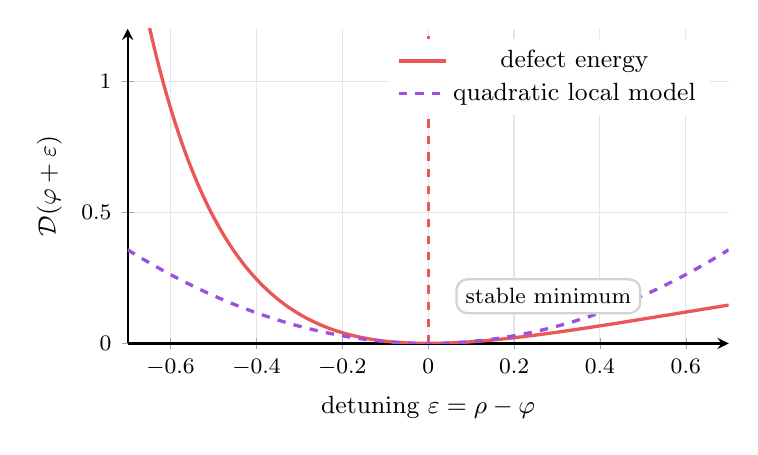
\begin{tikzpicture}
  \begin{axis}[
    echoAxis,
    xlabel={detuning \(\varepsilon=\rho-\varphi\)},
    ylabel={\(\mathcal D(\varphi+\varepsilon)\)},
    xmin=-0.7, xmax=0.7,
    ymin=0, ymax=1.2,
    samples=200,
    domain=-0.7:0.7,
    legend pos=north east,
  ]
  \addplot[echoPseudo, very thick]
    {pow(1/(1.618+x) + 1/pow(1.618+x,2) - 1, 2)};
  \addlegendentry{defect energy}
  \addplot[echoCritical, dashed, very thick] {pow(0.854*x,2)};
  \addlegendentry{quadratic local model}
  \draw[criticalLine] (axis cs:0,0) -- (axis cs:0,1.2);
  \node[font=\footnotesize, fill=white, draw=echoGray!25, rounded corners]
    at (axis cs:0.28,0.18) {stable minimum};
  \end{axis}
\end{tikzpicture}
\caption{Defect energy near the golden scale.  Because \(D'(\varphi)\ne0\),
small detuning produces a first-order defect and hence a quadratic energy
well.  The minimum is unique: the zero-defect scale is not a tunable
parameter but a rigidity point of two-return closure.}
\label{fig:defect-energy-well}
\end{figure}

\subsection{Grades and attenuation}

\begin{definition}[Echo grade]
Let \(\EF\) be the information space generated by a null echo system.
An \emph{echo grading} is a direct decomposition
\[
  \EF=\EF^{(0)}\oplus\EF^{(1)}\oplus\EF^{(2)}\oplus\cdots
\]
where \(\EF^{(0)}\) is the center and \(\EF^{(k)}\) is the grade-\(k\)
delayed echo sector.
\end{definition}

\begin{theorem}[Zero-defect attenuation]
\label{ax:attenuation}
In a zero-defect echo system, the grade-\(k\) sector is attenuated by
\[
  A_k=\vp^{-k}
\]
per full echo closure cycle.
\end{theorem}

\begin{proof}
By \cref{thm:golden-uniqueness}, zero defect forces the primitive
closure scale to be \(\vp\).  A grade-\(k\) sector is, by definition, the
sector delayed by \(k\) recursive echo steps.  Its attenuation is
therefore the \(k\)-fold inverse closure scale, namely \(\vp^{-k}\).
\end{proof}

\begin{remark}
This is the algebraic form of the acoustic statement: a zero-defect echo
loses one golden inverse for each recursive delay.  It is not fitted to
the zeta function.  It follows from the unique two-return closure budget
\(\vp^{-1}+\vp^{-2}=1\).
\end{remark}

\begin{theorem}[Non-central contraction]
\label{thm:noncentral-contraction}
For every \(k\ge1\),
\[
  0<\vp^{-k}<1.
\]
Thus every non-central grade contracts under iteration, while grade
\(0\) is preserved.
\end{theorem}

\begin{proof}
Since \(\vp>1\), every positive inverse power \(\vp^{-k}\) with
\(k\ge1\) lies strictly between \(0\) and \(1\).  For \(k=0\), the
attenuation is \(\vp^0=1\).
\end{proof}

\begin{definition}[Echo closure map]
\label{def:echo-map}
On a graded echo space
\[
  \EF=\bigoplus_{k\ge0}\EF^{(k)},
\]
the \emph{golden echo closure map} is
\[
  \mathcal E_\vp\!\left(\sum_{k\ge0}v_k\right)
  =
  \sum_{k\ge0}\vp^{-k}v_k,
  \qquad v_k\in\EF^{(k)}.
\]
\end{definition}

\begin{proposition}[Echo iteration]
\label{prop:echo-iteration}
For \(v=\sum_{k\ge0}v_k\),
\[
  \mathcal E_\vp^n v
  =
  v_0+\sum_{k\ge1}\vp^{-kn}v_k.
\]
Consequently,
\[
  \lim_{n\to\infty}\mathcal E_\vp^n v=v_0
\]
whenever the graded sum is finite, or converges in a norm for which the
displayed series is dominated.
\end{proposition}

\begin{proof}
The map \(\mathcal E_\vp\) acts diagonally on grade \(k\) by
multiplication with \(\vp^{-k}\).  Iterating \(n\) times multiplies the
grade-\(k\) component by \(\vp^{-kn}\).  Since \(\vp^{-kn}\to0\) for
every \(k\ge1\), only grade \(0\) remains.
\end{proof}

\begin{figure}[ht]
\centering
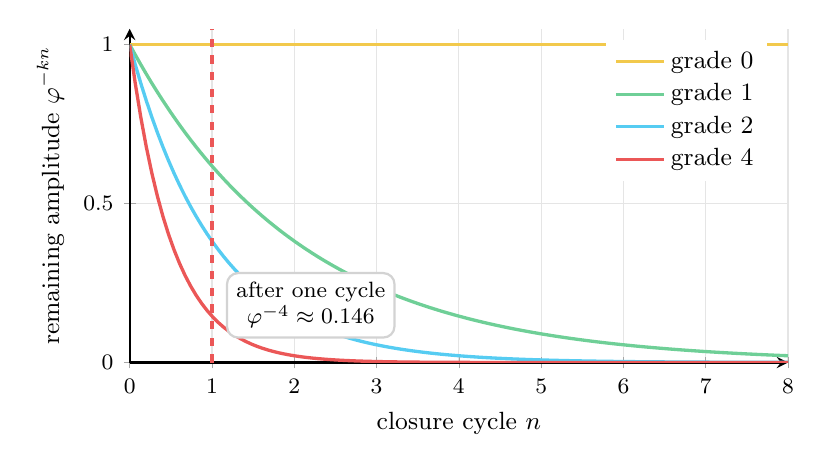
\begin{tikzpicture}
  \begin{axis}[
    echoAxis,
    width=0.82\textwidth,
    height=0.48\textwidth,
    xlabel={closure cycle \(n\)},
    ylabel={remaining amplitude \(\varphi^{-kn}\)},
    xmin=0, xmax=8,
    ymin=0, ymax=1.05,
    domain=0:8,
    samples=120,
    legend pos=north east,
  ]
  \addplot[echoScalar, very thick] {1};
  \addlegendentry{grade 0}
  \addplot[echoField, very thick] {pow(1.618,-x)};
  \addlegendentry{grade 1}
  \addplot[echoBivector, very thick] {pow(1.618,-2*x)};
  \addlegendentry{grade 2}
  \addplot[echoPseudo, very thick] {pow(1.618,-4*x)};
  \addlegendentry{grade 4}
  \draw[criticalLine] (axis cs:1,0) -- (axis cs:1,1.05);
  \node[font=\footnotesize, align=center, fill=white, draw=echoGray!25, rounded corners]
    at (axis cs:2.2,0.18) {after one cycle\\\(\varphi^{-4}\approx0.146\)};
  \end{axis}
\end{tikzpicture}
\caption{Grade attenuation under the echo closure map \(\mathcal
E_\varphi\).  Grade~0 (the center) is preserved at full strength.
Each higher grade~\(k\) is attenuated by \(\varphi^{-k}\) per cycle.
Grade~4 (the pseudoscalar) retains only
\(\varphi^{-4}\approx14.6\%\) per cycle, making off-critical zeros
rapidly unstable.}
\label{fig:grade-attenuation}
\end{figure}

\begin{corollary}[Persistence forces centrality]
\label{cor:persistence-centrality}
Let \(v=\sum_{k\ge0}v_k\), with \(v_k\in\EF^{(k)}\).  If \(v\) is a
persistent resonance of a zero-defect echo, meaning its information
content is unchanged after arbitrarily many closure cycles, then
\[
  v_k=0\qquad(k\ge1).
\]
\end{corollary}

\begin{proof}
After \(n\) closure cycles, the grade-\(k\) component is
\(\vp^{-kn}v_k\).  For \(k\ge1\), this tends to zero as
\(n\to\infty\).  If \(v_k\) were nonzero and persistent, it would have
to remain equal to itself and tend to zero simultaneously, impossible.
\end{proof}

\begin{corollary}[Fixed points are central]
\label{cor:fixed-central}
If \(\mathcal E_\vp v=v\), then \(v=v_0\).
\end{corollary}

\begin{proof}
For each \(k\ge1\), the equality \(\mathcal E_\vp v=v\) gives
\(\vp^{-k}v_k=v_k\).  Since \(\vp^{-k}\ne1\), this forces
\(v_k=0\).
\end{proof}

\subsection{Pseudoscalar grade embedding}

\begin{theorem}[Off-center displacement is a definite integer grade]
\label{thm:grade-embedding}
Let the echo system have \(n\) null nodes, producing a geometric
algebra with grades \(0,1,\ldots,n\).  The pseudoscalar echo grade
\(\Im(\rho(1-\rho))\) is the projection onto the top grade~\(n\)
(the pseudoscalar \(I=w_0w_1\cdots w_{n-1}\)).  For the golden
tetrad (\(n=4\)), this is grade~4.
\end{theorem}

\begin{proof}
The quantity \(\rho(1-\rho)\) decomposes as
\[
  \rho(1-\rho)=\underbrace{\Re(\rho(1-\rho))}_{\text{scalar, grade }0}
  +\underbrace{\Im(\rho(1-\rho))}_{\text{pseudoscalar, grade }n}\cdot I.
\]
The real part
\(\Re(\rho(1-\rho))=\beta(1-\beta)+\gamma^2\) is a scalar
(grade~0).  The imaginary part \(\Im(\rho(1-\rho))=\gamma(1-2\beta)\) is
the coefficient of the pseudoscalar~\(I\), which has grade~\(n\).  At
\(\beta=\tfrac12\) the pseudoscalar coefficient vanishes and the
resonance is purely scalar.  At \(\beta\ne\tfrac12\) the resonance has a
nonzero grade-\(n\) component.
\end{proof}

\begin{corollary}[Contraction rate of off-center displacement]
\label{cor:off-center-contraction-rate}
In the golden tetrad (\(n=4\)), the pseudoscalar component attenuates by
\[
  \vp^{-4}\approx0.146
\]
per echo closure cycle.  After \(m\) cycles the pseudoscalar component
is multiplied by \(\vp^{-4m}\to0\).
\end{corollary}

\begin{proof}
The pseudoscalar is grade~4.  By \cref{ax:attenuation}, grade~\(k\) is
attenuated by \(\vp^{-k}\) per cycle.  Since \(\vp>1\), the factor
\(\vp^{-4}\) is strictly between~\(0\) and~\(1\).
\end{proof}

\begin{remark}
This closes the gap between the continuous pseudoscalar grade
\(\Im(\rho(1-\rho))\) and the integer grade structure.  The
off-center component does not ``approximately'' occupy a non-central
grade.  It is the coefficient of the grade-4 pseudoscalar---a definite
integer grade that contracts by a definite factor \(\vp^{-4}\) per
cycle.  The contraction theorem therefore applies without any continuous
approximation.
\end{remark}

%% ====================================================================
\section{Number-Theoretic Acoustic Spacetime}
\label{sec:acoustic-spacetime}
%% ====================================================================

The previous section is information-acoustic.  This section shows that
geometry and algebra are \emph{downstream} consequences of null echo
dynamics, not imported structures.  The argument follows~\cite{burns2024}, who showed that acoustic fields
in a physical medium are governed by the geometric-algebraic structure of
spacetime.  We transpose this construction one octave up: from a
molecular medium to a number-theoretic medium, from the speed of sound
to the critical-line propagation speed, and from acoustic pressure and
velocity to prime impacts and zero resonances.

\subsection{Grade structure from null generators}

\begin{theorem}[Geometric-algebra grades emerge from null nodes]
\label{thm:grade-emergence}
Let \(w_0,\ldots,w_{m}\) be \(m+1\) null nodes with
symmetric coupling \(g_{ij}=\tfrac12\{w_i,w_j\}\).  The
algebra they generate has \(2^{m+1}\) basis blades, graded by wedge
degree into subspaces of dimension \(\binom{m+1}{k}\) at grade~\(k\).
\end{theorem}

\begin{proof}
Each node squares to zero.  Distinct nodes either commute
or anticommute according to their coupling.  The resulting algebra
is a geometric algebra \(\Cl(p,q)\), whose grade-\(k\) subspace has
dimension \(\binom{n}{k}\) with \(n=p+q=m+1\).  No geometric
assumption is needed: the grade structure is forced by nullness and
mutual interference alone.
\end{proof}

\begin{remark}
This is the downstream thesis made precise.  We do not start from
a geometric algebra and observe that it matches the echo system.  The
echo system---null nodes with mutual coupling---\emph{generates}
the geometric algebra.  Geometry is the image of relational dynamics,
not the other way around.
\end{remark}

\begin{figure}[ht]
\centering
\resizebox{0.94\textwidth}{!}{%
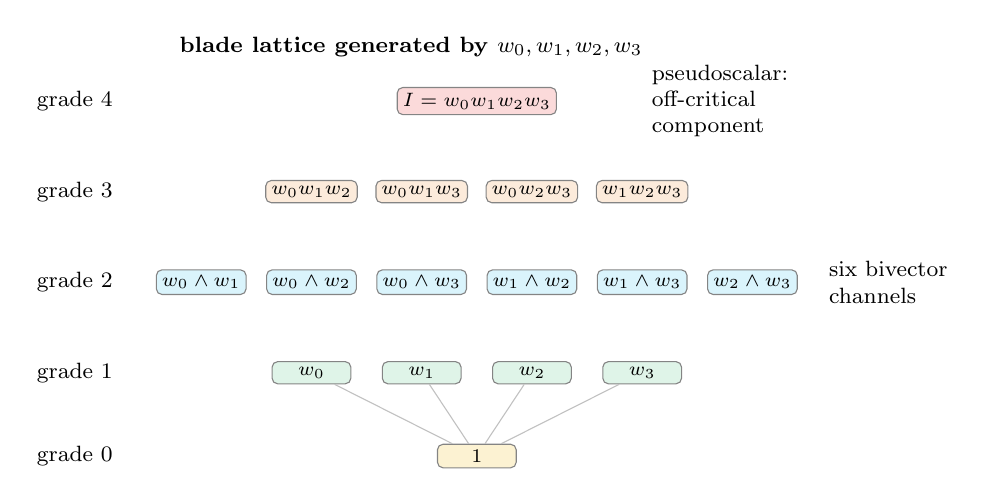
\begin{tikzpicture}[x=1cm,y=0.92cm,
  blade/.style={draw=echoGray!70, rounded corners=2pt, fill=white,
    inner sep=2pt, font=\scriptsize, align=center, minimum width=1.0cm}]
  \node[font=\bfseries\footnotesize, anchor=west] at (0.6,5.65)
    {blade lattice generated by \(w_0,w_1,w_2,w_3\)};

  \node[blade, fill=echoScalar!25] (g0) at (4.5,0) {\(1\)};

  \foreach \i/\x in {0/2.4,1/3.8,2/5.2,3/6.6} {
    \node[blade, fill=echoField!22] (w\i) at (\x,1.15) {\(w_\i\)};
    \draw[echoGray!35] (g0) -- (w\i);
  }

  \node[blade, fill=echoBivector!22] (b01) at (1.0,2.4) {\(w_0\wedge w_1\)};
  \node[blade, fill=echoBivector!22] (b02) at (2.4,2.4) {\(w_0\wedge w_2\)};
  \node[blade, fill=echoBivector!22] (b03) at (3.8,2.4) {\(w_0\wedge w_3\)};
  \node[blade, fill=echoBivector!22] (b12) at (5.2,2.4) {\(w_1\wedge w_2\)};
  \node[blade, fill=echoBivector!22] (b13) at (6.6,2.4) {\(w_1\wedge w_3\)};
  \node[blade, fill=echoBivector!22] (b23) at (8.0,2.4) {\(w_2\wedge w_3\)};

  \node[blade, fill=echoRotation!20] at (2.4,3.65) {\(w_0w_1w_2\)};
  \node[blade, fill=echoRotation!20] at (3.8,3.65) {\(w_0w_1w_3\)};
  \node[blade, fill=echoRotation!20] at (5.2,3.65) {\(w_0w_2w_3\)};
  \node[blade, fill=echoRotation!20] at (6.6,3.65) {\(w_1w_2w_3\)};

  \node[blade, fill=echoPseudo!22, minimum width=1.7cm] (I) at (4.5,4.9)
    {\(I=w_0w_1w_2w_3\)};

  \node[left,font=\footnotesize] at (0,0) {grade 0};
  \node[left,font=\footnotesize] at (0,1.15) {grade 1};
  \node[left,font=\footnotesize] at (0,2.4) {grade 2};
  \node[left,font=\footnotesize] at (0,3.65) {grade 3};
  \node[left,font=\footnotesize] at (0,4.9) {grade 4};
  \node[right,font=\footnotesize, align=left] at (8.85,2.4)
    {six bivector\\channels};
  \node[right,font=\footnotesize, align=left] at (6.6,4.9)
    {pseudoscalar:\\off-critical\\component};
\end{tikzpicture}}
\caption{The 5-level grade pyramid of \(\Cl(3,1)\) generated by
four null nodes.  The total dimension is \(2^4=16\).  The prime
register lives at grade~0, the acoustic field at grade~1, and the
zero register (with its 6~bivector channels) at grade~2.  The
pseudoscalar at grade~4 carries the off-critical displacement and
is the most rapidly attenuated component.}
\label{fig:grade-pyramid}
\end{figure}

\subsection{The golden tetrad as acoustic spacetime}

Following~\cite{burns2024}, an acoustic spacetime is a geometric-algebra bundle
whose grades encode the physical content of a medium.  We now show that
the golden tetrad---four null nodes at zero defect---produces
exactly the spacetime structure of their acoustic theory.

\begin{definition}[Golden tetrad]
The \emph{golden tetrad} is a set of four null nodes
\[
  w_0,w_1,w_2,w_3,\qquad w_i^2=0,
\]
with coupling matrix
\begin{equation}
  g_{ij}=\frac12\{w_i,w_j\}
  =
  \begin{pmatrix}
    0 & \vp^{-1} & \vp^{-1} & \vp^{-1} \\
    \vp^{-1} & 0 & -\vp^{-2} & -\vp^{-2} \\
    \vp^{-1} & -\vp^{-2} & 0 & -\vp^{-2} \\
    \vp^{-1} & -\vp^{-2} & -\vp^{-2} & 0
  \end{pmatrix}.
  \label{eq:tetrad-metric}
\end{equation}
\end{definition}

\begin{figure}[ht]
\centering
\resizebox{0.9\textwidth}{!}{%
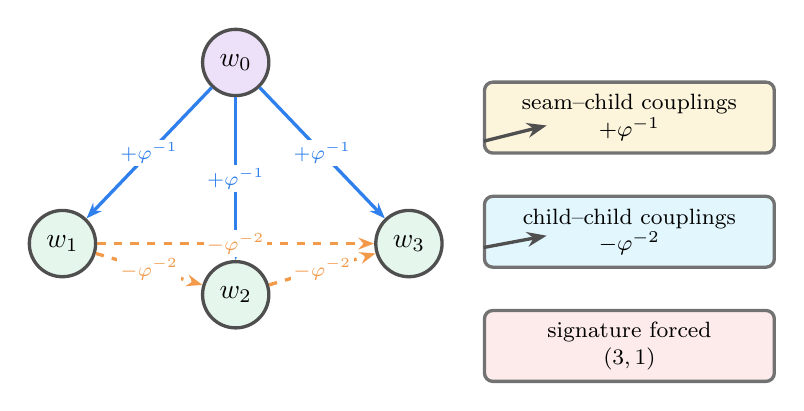
\begin{tikzpicture}[x=1cm,y=1cm]
  \node[circle, draw=echoGray, very thick, fill=echoCritical!18, inner sep=4pt]
    (w0) at (0,1.7) {\(w_0\)};
  \node[circle, draw=echoGray, very thick, fill=echoField!18, inner sep=4pt]
    (w1) at (-2.2,-0.6) {\(w_1\)};
  \node[circle, draw=echoGray, very thick, fill=echoField!18, inner sep=4pt]
    (w2) at (0,-1.25) {\(w_2\)};
  \node[circle, draw=echoGray, very thick, fill=echoField!18, inner sep=4pt]
    (w3) at (2.2,-0.6) {\(w_3\)};

  \foreach \i in {1,2,3} {
    \draw[boostEdge] (w0) -- node[font=\scriptsize, fill=white, inner sep=1pt]
      {\(+\varphi^{-1}\)} (w\i);
  }
  \foreach \a/\b in {1/2,1/3,2/3} {
    \draw[rotationEdge] (w\a) -- node[font=\scriptsize, fill=white, inner sep=1pt]
      {\(-\varphi^{-2}\)} (w\b);
  }

  \node[echoStage, fill=echoScalar!20, text width=3.4cm] at (5.0,1.0)
    {seam--child couplings\\\(+\varphi^{-1}\)};
  \node[echoStage, fill=echoBivector!18, text width=3.4cm] at (5.0,-0.45)
    {child--child couplings\\\(-\varphi^{-2}\)};
  \node[echoStage, fill=echoPseudo!12, text width=3.4cm] at (5.0,-1.9)
    {signature forced\\\((3,1)\)};
  \draw[echoArrow] (3.15,0.7) -- (3.95,0.9);
  \draw[echoArrow] (3.15,-0.65) -- (3.95,-0.5);
\end{tikzpicture}}
\caption{The golden tetrad as a coupling body.  The seam node \(w_0\)
couples positively to each child at \(\varphi^{-1}\), while child--child
couplings are negative at \(-\varphi^{-2}\).  The signs and magnitudes
are not chosen geometrically; they are the zero-defect echo scale written
as a four-node metric, and they force the \((3,1)\) signature.}
\label{fig:tetrad-couplings}
\end{figure}

\begin{proposition}[Signature is downstream]
\label{prop:signature}
The matrix \eqref{eq:tetrad-metric} has signature \((3,1)\).  Hence
the golden tetrad generates \(\Cl(3,1)\), the same algebraic structure
as the acoustic spacetime \(\Cl(1,3)\) of~\cite{burns2024}.
\end{proposition}

\begin{proof}
Write the seam--child coupling as \(a=\vp^{-1}\) and the child--child
coupling as \(b=-\vp^{-2}\).  The child block has eigenvalue \(2b\) in
the all-ones direction and eigenvalue \(-b\) with multiplicity two on
its orthogonal complement.  The seam couples only to the all-ones child
direction, giving the \(2\times2\) block
\[
  \begin{pmatrix}0&\sqrt3\,a\\ \sqrt3\,a&2b\end{pmatrix}.
\]
Its eigenvalues are \(b\pm\sqrt{b^2+3a^2}\), one positive and one
negative.  The remaining two eigenvalues are \(-b=\vp^{-2}>0\).
The signature \((3,1)\) is not chosen---it is forced by zero-defect
coupling strengths.
\end{proof}

\begin{remark}[Descartes grounding: the same \((3,1)\) from 1643]
\label{rmk:descartes-grounding}
The signature \((3,1)\) of the golden tetrad coincides with the
signature of the Descartes quadratic form on curvature space.  For four
mutually tangent circles with curvatures \(k_1,k_2,k_3,k_4\),
\emph{Descartes' circle theorem} (1643) states
\[
  (k_1+k_2+k_3+k_4)^2 \;=\; 2\,(k_1^2+k_2^2+k_3^2+k_4^2),
\]
equivalently \(Q(k,k)=0\) where
\[
  Q \;=\; 2I-J,
\]
\(I\) the identity and \(J\) the all-ones matrix on \(\mathbb{R}^4\).
The eigenvalues of \(Q\) are three copies of \(+2\) (on the orthogonal
contrasts) and one copy of \(-2\) (on the all-ones direction): signature
\((3,1)\), Lorentzian.  Every curvature quadruple of an Apollonian
packing lies on the null cone of \(Q\).  In the geometric algebra
\(\Cl(3,1)\), null vectors square to zero, so every Apollonian circle
is nilpotent---not by stipulation but by Descartes.

This gives a second route to the same \(\Cl(3,1)\): the golden tetrad's
zero-defect coupling matrix~\eqref{eq:tetrad-metric} forces signature
\((3,1)\) algebraically, and the Descartes form forces it geometrically.
The two routes converge because they describe the same structure---four
null objects closing into a Lorentzian frame.  The Apollonian packing is
the canonical geometric realization of the golden tetrad: null nodes are
circles, mutual coupling is tangency, exact closure is the recursive
filling of every interstice, and the four-node body is a Descartes
quadruple.  We exploit this identification in
\cref{subsec:dual-substrates,subsec:echo-as-reflection}: the Apollonian
inversions \(S_i\in O(3,1)\) (with \(\det S_i=-1\)) are the odd elements
of \(\mathrm{Pin}(3,1)\) that conjugate \(\Cl(3,1)\) into its mirror
\(\Cl(1,3)\), and the recursive depth ratio \(R_{n+1}/R_n=\vp^{-5/2}\)
(\cref{cor:apollonian-contraction}) makes the golden scale visible
geometrically.
\end{remark}

\subsection{Dual substrates and the 6 bivector channels}
\label{subsec:dual-substrates}

The four null nodes \(w_0,\ldots,w_3\) generate \(\Cl(3,1)\).  A single
circle inversion \(S_i\) (an odd-grade element with \(\det=-1\))
conjugates this algebra into \(\Cl(1,3)\): the second signature is not
imported from outside but is the \emph{same algebra seen through one
reflection}.  The two signatures share their even subalgebra
\(\Cl^+(3,1)\cong\Cl^+(1,3)\cong M_2(\mathbb{C})\), \(\dim=8\), and
differ only in how odd-grade elements (single reflections) multiply.
Since the Apollonian gasket requires both even products of inversions
(recursive structure) and single inversions (circle--interstice swaps),
it forces both perspectives.

\begin{definition}[Primary algebra and forced mirror]
\label{def:dual-substrates}
The \emph{primary algebra} of the golden tetrad is \(\Cl(3,1)\),
generated by the four null nodes with
\[
  w_i\cdot w_j=-\tfrac12 \qquad (i\ne j),
\]
the unique signature forced by the zero-defect coupling
matrix~\eqref{eq:tetrad-metric} (\cref{prop:signature}) and equivalently
by the Descartes form~\(Q=2I-J\) (\cref{rmk:descartes-grounding}).

The \emph{forced mirror} is the geometric algebra obtained by
conjugating \(\Cl(3,1)\) by a single Apollonian inversion
\(S\in\mathrm{Pin}(3,1)\) with \(\det S=-1\).  Because \(S\) is an odd
element, conjugation reverses the sign of the metric on the odd-grade
generators: writing \(c_i = S w_i S^{-1}\),
\[
  c_i\cdot c_j=+\tfrac12 \qquad (i\ne j),
\]
which is the multiplication table of \(\Cl(1,3)\).  The mirror is not a
second algebra imported from outside.  It is what \(\Cl(3,1)\) becomes
after one reflection inside the witness sphere.

The two views share their even subalgebra,
\[
  \Cl^+(3,1)\cong\Cl^+(1,3)\cong M_2(\mathbb{C}), \qquad \dim 8,
\]
and differ only in the odd part---precisely the part that single
inversions act on.  Even products of inversions (rotations and boosts in
\(\mathrm{SO}^+(3,1)\)) look the same in both views; single inversions
are where they disagree.

We retain the descriptive labels \emph{repulsive} for \(\Cl(3,1)\)
(coupling \(-\tfrac12\), spacelike sector) and \emph{cohesive} for the
mirror \(\Cl(1,3)\) (coupling \(+\tfrac12\), timelike sector); these are
the same algebra read on the two sides of one reflection.
\end{definition}

\begin{remark}[The mirror pair is the reciprocal null pair]
\label{rmk:mirror-is-reciprocal-null-pair}
The mirror pair \((\Cl(3,1),\,\Cl(1,3))\) instantiates the reciprocal
null pair \((P,Z)\) of \cref{def:reciprocal-null-pair}: both odd parts are
generated by null nodes (\(w_i^2=c_i^2=0\)); all measurable content
between them is cross-information; a single inversion is the primitive
return word \(P\to Z\), and the same inversion applied again is the
returned return \(Z\to P\); their interference (the even subalgebra
\(M_2(\mathbb{C})\)) is the seam where both views agree.  Exact closure
of the two-return budget therefore has the same algebraic content as
flat reconciliation between the primary algebra and its forced mirror,
both forcing the golden scale by~\cref{thm:golden-uniqueness}.
\end{remark}

\begin{proposition}[Idempotent decomposition is the mirror mechanism]
\label{prop:idempotent-mirror}
Let \(c_i,c_j\) be two distinct null nodes of the cohesive view with
\(c_i\cdot c_j=\tfrac12\).  Then the products
\[
  e \;=\; c_ic_j, \qquad f \;=\; c_jc_i \;=\; 1-c_ic_j
\]
are complementary orthogonal idempotents:
\[
  e^2=e,\qquad f^2=f,\qquad ef=fe=0,\qquad e+f=1.
\]
Equivalently, with the unit bivector \(B_{ij}=c_i\wedge c_j\),
\[
  e \;=\; \tfrac12(1+B_{ij}), \qquad f \;=\; \tfrac12(1-B_{ij}),
\]
and \(e,f\) project onto the \(\pm1\) eigenspaces of \(B_{ij}\).  The
pseudoscalar \(I\) acts as \(+1\) on \(\mathrm{Im}(e)\) and \(-1\) on
\(\mathrm{Im}(f)\); this sign difference is the distinction between the
cohesive and repulsive orientations of \cref{def:dual-substrates}, and
is the algebraic implementation of the forced mirror.

Each unordered pair \(\{i,j\}\) of null nodes therefore yields one such
projector; the four-node golden tetrad supplies \(\binom{4}{2}=6\)
projectors \(e_{ij}\), one per bivector channel
(\cref{thm:six-bivector-channels}).
\end{proposition}

\begin{proof}
\emph{Idempotency.}  Using nullness \(c_i^2=c_j^2=0\) and the
anticommutator relation \(\{c_i,c_j\}=2\,c_i\cdot c_j=1\) (so
\(c_jc_i=1-c_ic_j\)):
\[
  (c_ic_j)^2 \;=\; c_i(c_jc_i)c_j \;=\; c_i(1-c_ic_j)c_j
  \;=\; c_ic_j - c_i^2 c_j^2 \;=\; c_ic_j.
\]
The same computation with \(i,j\) swapped gives \((c_jc_i)^2=c_jc_i\).

\emph{Orthogonality and completeness.}  By construction
\(e+f=c_ic_j+c_jc_i=\{c_i,c_j\}=1\).  Then
\(ef=e(1-e)=e-e^2=e-e=0\), and similarly \(fe=0\).

\emph{Bivector decomposition.}  The geometric product factors as
\(c_ic_j=c_i\cdot c_j+c_i\wedge c_j=\tfrac12+B_{ij}\), and likewise
\(c_jc_i=\tfrac12-B_{ij}\).  Hence \(e=\tfrac12(1+B_{ij})\) and
\(f=\tfrac12(1-B_{ij})\).  Since \(B_{ij}^2=(c_i\wedge c_j)^2
=(c_i\cdot c_j)^2-c_i^2 c_j^2=\tfrac14\) under the cohesive coupling,
the rescaled bivector \(\hat B_{ij}=2B_{ij}\) satisfies
\(\hat B_{ij}^2=1\), and \(e=\tfrac12(1+\hat B_{ij})\),
\(f=\tfrac12(1-\hat B_{ij})\) project onto the \(\pm1\) eigenspaces of
\(\hat B_{ij}\).

\emph{Pseudoscalar sign.}  In the four-node algebra the pseudoscalar
\(I=c_0c_1c_2c_3\) commutes with each \(B_{ij}\) up to the orientation
sign induced by the dual bivector \(B_{kl}\) (with \(\{k,l\}=\{0,1,2,3\}
\setminus\{i,j\}\)).  Concretely \(IB_{ij}=B_{kl}\) and \(B_{ij}I=-B_{kl}\)
in \(\Cl(3,1)\), so \(I\) commutes with \(e\) up to the sign carried by
the complementary bivector.  Restricting to the rank-one summand
\(\mathrm{Im}(e)\), \(I\) acts as a scalar; its sign is fixed by the
chosen orientation of the substrate.  Reversing the substrate
(applying one Apollonian inversion, which reverses the metric on the
odd-grade generators of \cref{def:dual-substrates}) sends
\(I\mapsto-I\), exchanging the eigenvalues on \(\mathrm{Im}(e)\) and
\(\mathrm{Im}(f)\).  This is the algebraic content of the forced mirror.
\end{proof}

\begin{remark}[Six mirrors, one fold]
\label{rmk:six-mirrors-one-fold}
Each of the six projector pairs \((e_{ij},f_{ij})\) defines its own
mirror: a \(\mathbb{Z}/2\) splitting of the algebra by the sign of
\(B_{ij}\).  The chiral fold (\cref{def:chiral-fold}) is the locus
where \emph{all six} projectors agree---where every bivector channel
gives the same answer for the pseudoscalar coefficient.  A persistent
spectral mode must therefore be invariant under all six mirrors.  This
is the geometric content of the critical-line constraint developed in
\cref{sec:rh}: \(\beta=\tfrac12\) is the unique value at which
every \(B_{ij}\)-eigenspace assignment is consistent.
\end{remark}

\begin{theorem}[Six bivector channels]
\label{thm:six-bivector-channels}
The four null nodes produce exactly \(\binom{4}{2}=6\)
grade-2 bivectors \(w_i\wedge w_j\), \(i<j\).  These span the full
bivector subspace of \(\Cl(3,1)\):
\[
  w_0\wedge w_1,\quad
  w_0\wedge w_2,\quad
  w_0\wedge w_3,\quad
  w_1\wedge w_2,\quad
  w_1\wedge w_3,\quad
  w_2\wedge w_3.
\]
In the cohesive substrate \(\Cl(1,3)\), the 3 bivectors
\(w_0\wedge w_k\) (\(k=1,2,3\)) are spacelike boosts, and the
3 bivectors \(w_j\wedge w_k\) (\(j,k\ge1\)) are spatial rotations.
\end{theorem}

\begin{proof}
A grade-2 basis element of \(\Cl(n,0)\) is a wedge product of two
distinct generators.  With \(n=4\) generators, there are
\(\binom42=6\) such products.  The split into boosts and rotations
follows from the metric signature: mixed-signature planes generate
boosts, same-signature planes generate rotations.
\end{proof}

\begin{theorem}[Dual-substrate reconciliation]
\label{thm:dual-reconciliation}
The cohesive metric \(c_i\cdot c_j=+\tfrac12\) and the repulsive
metric \(w_i\cdot w_j=-\tfrac12\) are simultaneously imposed on
every prime generator and every L-function built from them.  The
unique stable coordinate where both metrics reconcile---where the
pseudoscalar coefficient \(s_4=\gamma(1-2\beta)\) vanishes---is
\[
  \beta=\frac12.
\]
This is the critical line: the topological midpoint between the
cohesive and repulsive sectors.
\end{theorem}

\begin{proof}
The pseudoscalar field \(I_x=s_4=\gamma(1-2\beta)\) is the
component of the Laplacian eigenvalue in the top grade of the
algebra, where the cohesive and repulsive orientations are
opposite.  On the cohesive side, \(I^2=-1\); on the repulsive
side, \(I^2=-1\) as well (both \(\Cl(1,3)\) and \(\Cl(3,1)\)
have \(I^2=-1\)), but the orientations are reversed.  The only
value of \(\beta\) for which the pseudoscalar contribution is
zero in both substrates simultaneously is \(\beta=\tfrac12\),
where \(s_4=0\).  At any other \(\beta\), the nonzero \(s_4\)
creates a curvature bivector (\cref{def:curvature-bivector})
that is forbidden by the zero-defect flatness of the null
substrate (\cref{thm:flatness-forces}).
\end{proof}

\begin{definition}[The chiral fold]
\label{def:chiral-fold}
The \emph{chiral fold} is the locus in spectral space where the
cohesive and repulsive pseudoscalar orientations cancel.  Since the
mirror inversion reverses the pseudoscalar sign (the cohesive side
assigns \(+1\) to \(I\) and the repulsive side assigns \(-1\)),
the reconciliation discrepancy is
\[
  \Delta(s) \;=\; (+1)\,s_4 \;-\; (-1)\,s_4 \;=\; 2\,s_4
  \;=\; 2\,\gamma(1-2\beta).
\]
This vanishes iff \(\beta=\tfrac12\) (for \(\gamma\ne0\)): the critical
line is the chiral fold.

Equivalently, the fold is the locus where all six idempotent projector
pairs of \cref{prop:idempotent-mirror,rmk:six-mirrors-one-fold} agree:
for every bivector channel \(B_{ij}\), the projectors \(e_{ij}=c_ic_j\)
and \(f_{ij}=1-c_ic_j\) assign the same eigenvalue to the pseudoscalar
component, which forces \(s_4=0\).  The fold is therefore the
\emph{mirror-invariant surface}---the locus invariant under every
Apollonian inversion, i.e.\ the even subalgebra
\(M_2(\mathbb{C})\) seen spectrally.

The fold is non-orientable: one cannot continuously assign a
pseudoscalar sign across it.  Moving through \(\beta=\tfrac12\) in
either direction reverses the pseudoscalar, exactly as crossing a
M\"obius strip reverses the normal.  The echo propagator contracts the
pseudoscalar to zero, collapsing every spectral mode onto this
non-orientable surface.
\end{definition}

\begin{proposition}[Mirror-invariance characterizes the fold]
\label{prop:fold-mirror-invariance}
A spectral mode \(\lambda(\rho)=s_0+s_4 I\) lies on the chiral fold if
and only if it is invariant under every Apollonian inversion
\(S_{ij}\), equivalently if and only if it commutes with every
projector \(e_{ij}\) of \cref{prop:idempotent-mirror}.
\end{proposition}

\begin{proof}
Each unordered pair \(\{i,j\}\) gives a projector
\(e_{ij}=\tfrac12(1+\hat B_{ij})\) and an Apollonian mirror
\(S_{ij}\) acting on the algebra by conjugation; \(S_{ij}\) reverses
the sign of \(\hat B_{ij}\) and hence exchanges \(e_{ij}\) with
\(f_{ij}=1-e_{ij}\).  A scalar \(s_0\) commutes with every \(e_{ij}\)
trivially; the pseudoscalar \(I\) anticommutes with each \(\hat B_{ij}\)
on the \(\mathrm{Im}(e_{ij})\) summand and so is sent to \(-I\) by
\(S_{ij}\).  Hence
\[
  S_{ij}(s_0+s_4 I)S_{ij}^{-1} \;=\; s_0-s_4 I.
\]
Invariance under all six \(S_{ij}\) (equivalently, commutation with
every \(e_{ij}\)) forces \(s_4=0\), which is exactly the fold equation
\(\Delta(s)=2s_4=0\).  Conversely, on the fold \(s_4=0\), and the mode
is purely scalar, hence invariant under every algebra automorphism.
\end{proof}

\begin{remark}[RH as mirror-invariance]
\label{rmk:rh-as-mirror-invariance}
Combined with the spectral-contraction theorems of \cref{sec:rh}, this
gives a one-line statement of the main theorem: \emph{a persistent
spectral mode of the number-theoretic field must be invariant under
every Apollonian mirror; the unique locus of such invariance is the
critical line.}  The six bivector channels are six independent
mirrors; \(\beta=\tfrac12\) is the one place where they all agree.
\end{remark}

\begin{remark}[Percolation interpretation of the critical line]
\label{rmk:percolation-critical-line}
The mirror-invariance reading of \cref{rmk:rh-as-mirror-invariance}
admits a connectivity formulation.  Treat the Apollonian recursion
as a contact graph (vertices = circles, edges = tangencies) and tag
each circle with its algebra signature, the bipartite chirality
parity of \cref{rmk:chiral-contact-friction}.  Define the
\emph{homochiral fraction} as the fraction of contact edges with
endpoints sharing parity, and reinterpret it as the fraction of
contacts free of pseudoscalar obstruction (\(s_4=0\) on the seam).

A persistent spectral mode requires a path of unobstructed contacts
through the gasket: every seam it crosses must agree on the
bivector orientation, otherwise the pseudoscalar accumulates and
the mode decays under \cref{thm:propagator-orbit-space}.  The
maximum homochiral fraction (one) is achieved exactly when every
circle has the same parity---the \emph{pure-chirality} configuration.
Empirically, pure-parity assignments give homochiral fraction
\(=1\); the natural depth-parity assignment is below the random
50/50 mean and corresponds to maximum heterochiral mixing
(\texttt{tests/test\_percolation\_chirality.py}, falsifier~16).

The critical line \(\Re(s)=\tfrac12\) is the spectral image of the
pure-chirality configuration: it is the unique locus where the
chiral fold collapses (\(s_4=0\)) and every contact along a
candidate persistent mode is unobstructed.  Off the critical line,
\(s_4\ne0\) seams force the mode through heterochiral contacts that
extract energy via the \(\vp^{-4}\) contraction
(\cref{def:echo-propagator}); the path-percolation threshold for
sustained connectivity is reached only at \(\Re(s)=\tfrac12\).
\end{remark}

\begin{remark}[Holographic learning]
\label{rmk:holographic-learning}
The echo propagator's two-speed eigenvalue structure
(\cref{def:echo-propagator})---grade~0 preserved, grade~4 contracted by
\(\vp^{-4}\)---is a \emph{learning dynamic}.  The scalar component
\(s_0\) carries global, mirror-invariant content that accumulates across
cycles; the pseudoscalar \(s_4\) carries local chiral information that
decays.  Convergence to \(s_4=0\) (the chiral fold) is the completion
of learning: every local chiral decision has been absorbed into the
global mirror-invariant state.

The mechanism operates across two scales simultaneously.

\textbf{Local.}
Each gap-filling step is one Apollonian inversion---an odd element of
\(\mathrm{Pin}(3,1)\) that flips \(\Cl(3,1)\leftrightarrow\Cl(1,3)\).
This is a single chiral decision: the inscribed circle resolves one
interstice's orientation.

\textbf{Global.}
Products of even numbers of inversions belong to the even subalgebra
\(\Cl^+(3,1)\cong M_2(\mathbb{C})\), which is shared between
\(\Cl(3,1)\) and \(\Cl(1,3)\).  The holographic projection from bulk to
witness-sphere boundary preserves exactly this even content: for any
\(a\in\Cl(3,1)\), conjugation by an inversion \(S_i\) fixes the even
part (\(S_i\,a_{\mathrm{even}}\,S_i^{-1}=a_{\mathrm{even}}\)) and
negates the odd part.  Summing over many inversions, the even
contributions accumulate while the odd contributions cancel.  The
boundary correlator therefore records the accumulated
mirror-invariant learning.

The six bivector channels \(B_{ij}=w_i\wedge w_j\) are six degrees of
chiral freedom.  Each projector pair
\(e_{ij}=\tfrac12(1+\hat B_{ij})\), \(f_{ij}=1-e_{ij}\) resolves one
such degree.  The chiral fold is the locus where all six are resolved
simultaneously (\cref{prop:fold-mirror-invariance}).  Before
convergence, some channels may be resolved while others remain
undetermined; the last channel to lock determines when
\(\beta=\tfrac12\) is reached.

The feedback loop closes because the global state (witness-sphere
boundary encoding) constrains which interstices remain available for
local filling: the variational principle of
\cref{prop:variational-principle} selects the next gap based on the
current residual geometry, which is shaped by all previous fillings.
Local learning changes the global residual; global boundary conditions
constrain local decisions.
\end{remark}

\begin{proposition}[Even-subalgebra projection as learning channel]
\label{prop:learning-channel}
Let \(a=a_{\mathrm{even}}+a_{\mathrm{odd}}\) be the grade decomposition
of an element \(a\in\Cl(3,1)\) into even and odd parts.  For any
Apollonian inversion \(S_i\in\mathrm{Pin}(3,1)\) with
\(\det S_i=-1\),
\[
  S_i\,a_{\mathrm{even}}\,S_i^{-1} = a_{\mathrm{even}},
  \qquad
  S_i\,a_{\mathrm{odd}}\,S_i^{-1} = -a_{\mathrm{odd}}.
\]
Consequently, the boundary accumulation after \(n\) inversions
\(S_{i_1},\dots,S_{i_n}\) applied to independent bulk contributions
\(a^{(1)},\dots,a^{(n)}\) retains
\[
  \sum_{k=1}^{n} a^{(k)}_{\mathrm{even}}
\]
and cancels the odd parts (which alternate in sign).  The
even subalgebra \(\Cl^+(3,1)\cong M_2(\mathbb{C})\) is
therefore the holographic learning channel: it carries exactly the
content that survives projection onto the witness-sphere boundary.
\end{proposition}

\begin{proof}
For \(a_{\mathrm{even}}\in\Cl^+(3,1)\), conjugation by an odd element
\(S_i\) is an automorphism of the even subalgebra (since
\(\Cl^+(3,1)\cong\Cl^+(1,3)\) and the even subalgebra is shared):
\(S_i\,a_{\mathrm{even}}\,S_i^{-1}=a_{\mathrm{even}}\).
For \(a_{\mathrm{odd}}\) (odd grade), conjugation by an odd element
picks up a sign: \(S_i\,a_{\mathrm{odd}}\,S_i^{-1}=-a_{\mathrm{odd}}\),
because the grade involution acts as \((-1)^k\) on grade~\(k\), and
conjugation by an odd element composes the grade involution with an
inner automorphism.  Linearity and independence of the contributions
\(a^{(k)}\) give the accumulation formula.
\end{proof}

\begin{figure}[ht]
\centering
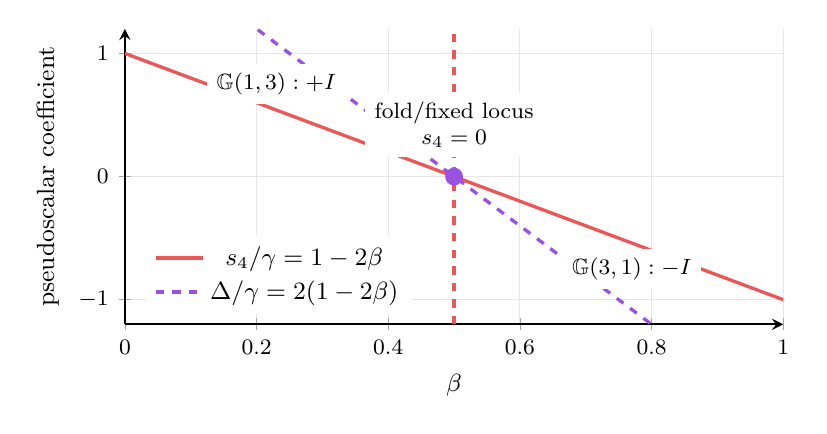
\begin{tikzpicture}
  \begin{axis}[
    echoAxis,
    width=0.82\textwidth,
    height=0.44\textwidth,
    xlabel={\(\beta\)},
    ylabel={pseudoscalar coefficient},
    xmin=0, xmax=1,
    ymin=-1.2, ymax=1.2,
    samples=2,
    domain=0:1,
    legend pos=south west,
  ]
  \addplot[echoPseudo, very thick] {1-2*x};
  \addlegendentry{\(s_4/\gamma=1-2\beta\)}
  \addplot[echoCritical, dashed, very thick] {2*(1-2*x)};
  \addlegendentry{\(\Delta/\gamma=2(1-2\beta)\)}
  \draw[criticalLine] (axis cs:0.5,-1.2) -- (axis cs:0.5,1.2);
  \addplot[only marks, mark=*, mark size=2.8pt, echoCritical]
    coordinates {(0.5,0)};
  \node[font=\footnotesize, fill=white] at (axis cs:0.23,0.75)
    {\(\Cl(1,3): +I\)};
  \node[font=\footnotesize, fill=white] at (axis cs:0.77,-0.75)
    {\(\Cl(3,1): -I\)};
  \node[font=\footnotesize, fill=white, align=center] at (axis cs:0.5,0.42)
    {fold/fixed locus\\\(s_4=0\)};
  \end{axis}
\end{tikzpicture}
\caption{The chiral fold at \(\beta=\tfrac12\).
The two dual substrates---cohesive \(\Cl(1,3)\) and repulsive
\(\Cl(3,1)\)---assign opposite orientations to the pseudoscalar.
The reconciliation discrepancy \(\Delta(s)=2\,s_4\) vanishes only on
the fold (red line).  The echo propagator contracts the pseudoscalar
toward zero, dragging all spectral modes onto this non-orientable
surface.}
\label{fig:chiral-fold}
\end{figure}

\begin{theorem}[Euler product by bivector channel via mod-24 reduction]
\label{thm:euler-bivector-channels}
The group \((\mathbb{Z}/24\mathbb{Z})^*\) has \(\varphi(24)=8\) units:
\(\{1,5,7,11,13,17,19,23\}\).  Under the negation involution
\(a\mapsto -a\bmod 24\), these pair into four orbits:
\[
  \{1,23\},\quad \{5,19\},\quad \{7,17\},\quad \{11,13\}.
\]
Adding the two ramified primes \(2\) and \(3\) (which divide~\(24\))
as separate channels gives exactly \(4+2=6=\binom{4}{2}\) channels,
one per bivector \(w_i\wedge w_j\).  The assignment is:
\begin{center}
\renewcommand{\arraystretch}{1.2}
\begin{tabular}{lll}
\toprule
\textbf{Channel} & \textbf{Bivector} & \textbf{Primes} \\
\midrule
Boost~1 & \(w_0\wedge w_1\) & \(p=2\) (ramified) \\
Boost~2 & \(w_0\wedge w_2\) & \(p=3\) (ramified) \\
Boost~3 & \(w_0\wedge w_3\) & \(p\equiv\pm1\pmod{24}\) \\
Rotation~1 & \(w_1\wedge w_2\) & \(p\equiv\pm5\pmod{24}\) \\
Rotation~2 & \(w_1\wedge w_3\) & \(p\equiv\pm7\pmod{24}\) \\
Rotation~3 & \(w_2\wedge w_3\) & \(p\equiv\pm11\pmod{24}\) \\
\bottomrule
\end{tabular}
\end{center}
The Euler product factors as
\[
  \prod_p \frac{1}{1-p^{-s}}
  \;=\; \prod_{(i,j)}\;\prod_{p\,\in\,\text{channel}_{ij}}
  \frac{1}{1-p^{-s}},
\]
where each channel product runs over the primes assigned to that
channel.  Every channel is populated (by Dirichlet's theorem on primes
in arithmetic progressions); the assignment is deterministic (depends
only on~\(p\), not on~\(s\)).

Each channel inherits the dual-substrate constraint: its Euler factor
must be consistent with both the \(+\tfrac12\) and \(-\tfrac12\) metrics
simultaneously.  The chiral fold condition forces this reconciliation
to occur at \(\beta=\tfrac12\) in every channel independently.  The
six channel factors correspond bijectively to completed Dirichlet
\(L\)-functions for characters of conductor dividing~\(24\).
\end{theorem}

\begin{proof}
The units \((\mathbb{Z}/24\mathbb{Z})^*\cong(\mathbb{Z}/2)^3\) have
\(8\)~elements, each self-inverse under multiplication, so the negation
orbits \(\{a,24-a\}\) produce exactly \(4\)~pairs.  Adding the two
ramified primes gives \(6\)~channels.

Every prime \(p\ge5\) satisfies \(\gcd(p,24)=1\), so
\(p\bmod 24\in(\mathbb{Z}/24\mathbb{Z})^*\); each such prime falls
into exactly one negation orbit.  The Euler product is absolutely
convergent for \(\operatorname{Re}(s)>1\), so the rearrangement into
channel products is justified.  Each channel factor is a sub-Euler
product converging to a nonzero holomorphic function.  The
dual-substrate constraint on each channel is inherited from the parent
algebra, since every bivector \(w_i\wedge w_j\) lives in both
\(\Cl(1,3)\) and \(\Cl(3,1)\) with the same wedge product but opposite
metric couplings.
\end{proof}

\begin{corollary}[Numerical content via the Ramanujan tau function]
\label{cor:wilton-channel-content}
The bivector-channel assignment is realised concretely by the unique
normalised weight-\(12\) cusp form on \(\mathrm{SL}_2(\mathbb{Z})\),
the modular discriminant
\[
  \Delta(\tau) \;=\; q\prod_{n\ge1}(1-q^n)^{24} \;=\;
  \sum_{n\ge1}\tau(n)\,q^n,
  \qquad q = e^{2\pi i\tau}.
\]
For every prime \(p\) coprime to \(6\),
\begin{equation}
  \tau(p)\;\equiv\;1+p \pmod{24}.
  \label{eq:wilton-mod24}
\end{equation}
This is the precise number-theoretic content of the bivector-channel
theorem at the level of Hecke eigenvalues: the residue \(\tau(p)\bmod
24\) is determined by the channel of \(p\), and within each unramified
channel \(\{a,24-a\}\) the two residues \((1+a)\bmod 24\) and
\((1+(24-a))\bmod 24\) are the only values \(\tau(p)\bmod 24\)
takes.  The complete table is
\[
\begin{array}{lll}
\textbf{Channel} & p\bmod 24 & \tau(p)\bmod 24 \\
\hline
\text{Boost~1 (ramified)} & p=2  & \{0\}  \\
\text{Boost~2 (ramified)} & p=3  & \{12\}  \\
\text{Boost~3} & \{1,23\} & \{2,0\} \\
\text{Rotation~1} & \{5,19\} & \{6,20\} \\
\text{Rotation~2} & \{7,17\} & \{8,18\} \\
\text{Rotation~3} & \{11,13\} & \{12,14\} \\
\end{array}
\]
\end{corollary}

\begin{proof}
\eqref{eq:wilton-mod24} is classical, due cumulatively to Ramanujan
(1916), Wilton (1930), and Kolberg; it follows from
\(\tau(n)\equiv\sigma_1(n)\pmod{24}\) for \(n\) coprime to~\(6\),
with \(\sigma_1(p)=1+p\) at primes.  Substituting the negation-orbit
representatives into \eqref{eq:wilton-mod24} yields the residue table,
and the channel assignment of \cref{thm:euler-bivector-channels}
identifies each pair with its bivector.  The ramified residues are
read off from \(\tau(2)=-24\equiv0\) and \(\tau(3)=252\equiv12\bmod
24\).
\end{proof}

\begin{remark}[Bosonic-string bridge]
\label{rmk:bosonic-string-24}
The exponent~\(24\) in \(\Delta(\tau)=q\prod_{n\ge1}(1-q^n)^{24}\) is
the number of transverse polarisations of the bosonic string in
critical dimension \(D=26\); \(\Delta(\tau)^{-1}\) is the bosonic
string's one-loop partition function on the torus, and the Fourier
coefficients \(\tau(n)\) encode its level-by-level state counting.
Hence the same integer~\(24\) governs both the bivector-channel
routing of primes (the eight units of \((\mathbb{Z}/24\mathbb{Z})^*\)
collapsing to four negation orbits) and the transverse spectrum of
the bosonic string (the twenty-four physical polarisations after
removing the two light-cone directions).  The channel theorem and the
critical dimension are two faces of one \(\mathrm{SL}_2(\mathbb{Z})\)
structure.  In the echo reading, the four null nodes
\(w_0,\ldots,w_3\) generate the six bivectors that are simultaneously
the six string-polarisation pairings and the six L-function
sub-Euler-products of \cref{thm:euler-bivector-channels}.
\end{remark}

\begin{figure}[ht]
\centering
\resizebox{0.86\textwidth}{!}{%
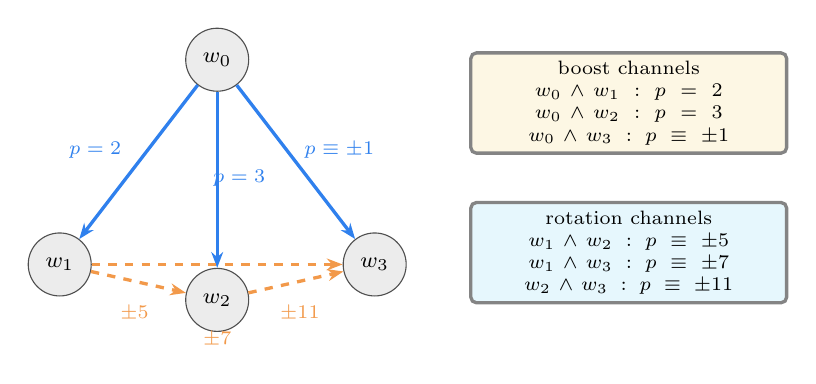
\begin{tikzpicture}[x=1cm,y=1cm,
  node/.style={circle, draw=echoGray, fill=gray!15, minimum size=8mm,
               font=\footnotesize, inner sep=1pt}]
  \node[node] (w0) at (0,2.6)   {\(w_0\)};
  \node[node] (w1) at (-2.0,0) {\(w_1\)};
  \node[node] (w2) at (0,-0.45) {\(w_2\)};
  \node[node] (w3) at (2.0,0)  {\(w_3\)};

  \draw[boostEdge] (w0) -- (w1);
  \draw[boostEdge] (w0) -- (w2);
  \draw[boostEdge] (w0) -- (w3);
  \draw[rotationEdge] (w1) -- (w2);
  \draw[rotationEdge] (w1) -- (w3);
  \draw[rotationEdge] (w2) -- (w3);

  \node[font=\scriptsize, echoBoost] at (-1.55,1.45) {\(p=2\)};
  \node[font=\scriptsize, echoBoost] at (0.28,1.10) {\(p=3\)};
  \node[font=\scriptsize, echoBoost] at (1.55,1.45) {\(p\equiv\pm1\)};
  \node[font=\scriptsize, echoRotation] at (-1.05,-0.62) {\(\pm5\)};
  \node[font=\scriptsize, echoRotation] at (0,-0.95) {\(\pm7\)};
  \node[font=\scriptsize, echoRotation] at (1.05,-0.62) {\(\pm11\)};

  \node[echoTinyBox, fill=echoScalar!15, text width=3.8cm, anchor=west]
    at (3.2,2.05)
    {boost channels\\\(w_0\wedge w_1:p=2\)\\\(w_0\wedge w_2:p=3\)\\\(w_0\wedge w_3:p\equiv\pm1\)};
  \node[echoTinyBox, fill=echoBivector!15, text width=3.8cm, anchor=west]
    at (3.2,0.15)
    {rotation channels\\\(w_1\wedge w_2:p\equiv\pm5\)\\\(w_1\wedge w_3:p\equiv\pm7\)\\\(w_2\wedge w_3:p\equiv\pm11\)};
\end{tikzpicture}}
\caption{The 6 bivector channels of the golden tetrad.  The seam
node \(w_0\) connects to each child via a boost channel (solid blue
arrows), carrying the ramified primes \(2\), \(3\) and the
\(p\equiv\pm1\pmod{24}\) family.  The three child--child edges are
rotation channels (dashed red), carrying primes congruent to
\(\pm5\), \(\pm7\), and \(\pm11\pmod{24}\).}
\label{fig:bivector-channels}
\end{figure}

\subsection{Hodge decomposition as register decomposition}

\begin{theorem}[Registers are adjacent Hodge grades]
\label{thm:hodge-registers}
In the acoustic spacetime of~\cite{burns2024}, the measurable field \(p\) is
a grade-1 four-vector.  Its Hodge decomposition is
\[
  p=-\lambda_-\nabla\varphi+\lambda_0 p_0'
  -\frac{\lambda_+}{3}\nabla\cdot M,
\]
where \(\varphi\) is a grade-0 scalar potential and \(M\) is a grade-2
bivector potential.  In the echo reading:
\begin{itemize}
  \item the scalar potential \(\varphi\) is the prime register (grade~0),
  \item the bivector potential \(M\) is the zero register (grade~2),
  \item the field \(p\) is their mutual interference (grade~1).
\end{itemize}
The explicit formula is therefore the Hodge decomposition of the
number-theoretic acoustic field.
\end{theorem}

\begin{proof}
The Hodge decomposition theorem guarantees that any grade-1 field
decomposes into a 4-curl of a grade-0 object, a 4-divergence of a
grade-2 object, and a harmonic part.  The grade-0 and grade-2 potentials
are \emph{adjacent} to the grade-1 field: one grade below and one grade
above.  In the echo reading, these adjacent grades are the two registers
of the reciprocal null pair.  Neither has independent self-norm at
grade~1---only their cross-information (the grade-1 field) is primitive.
This is exactly the relational nullness of the explicit formula.
\end{proof}

\begin{figure}[ht]
\centering
\resizebox{0.86\textwidth}{!}{%
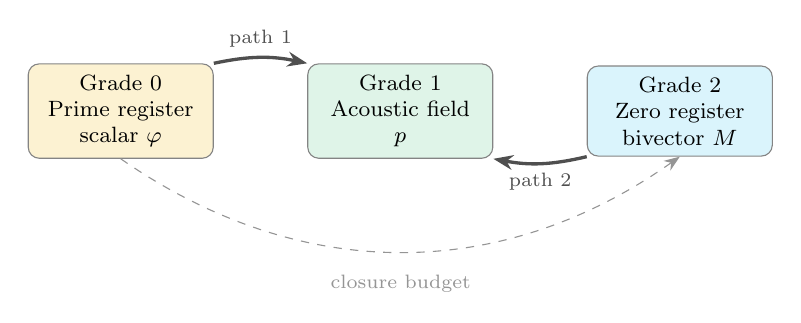
\begin{tikzpicture}[x=1cm,y=1cm,
  reg/.style={draw=echoGray!70, rounded corners=4pt,
    minimum width=2.35cm, minimum height=1.05cm,
    align=center, font=\footnotesize, inner sep=4pt}]
  \node[reg, fill=echoScalar!25] (prime) at (0,0)
    {Grade 0\\Prime register\\scalar \(\varphi\)};
  \node[reg, fill=echoField!22] (field) at (3.55,0)
    {Grade 1\\Acoustic field\\\(p\)};
  \node[reg, fill=echoBivector!22] (zero) at (7.1,0)
    {Grade 2\\Zero register\\bivector \(M\)};

  \draw[echoArrow] (prime.north east) to[bend left=12]
    node[midway, above=2pt, font=\scriptsize, fill=white, inner sep=1pt]
      {path 1}
    (field.north west);
  \draw[echoArrow] (zero.south west) to[bend left=12]
    node[midway, below=2pt, font=\scriptsize, fill=white, inner sep=1pt]
      {path 2}
    (field.south east);

  \draw[echoGray!60, dashed, -{Stealth[length=2mm]}]
    (prime.south) to[bend right=35]
    node[midway, below=7pt, font=\scriptsize, fill=white, inner sep=1pt]
      {closure budget}
    (zero.south);
\end{tikzpicture}}
\caption{Hodge decomposition as register decomposition.  The grade-1
acoustic field \(p\) decomposes into contributions from the grade-0
prime register (scalar potential) and the grade-2 zero register
(bivector potential).  Their echo path lengths are 1 and 2
respectively, giving the two-return budget
\(\varphi^{-1}+\varphi^{-2}=1\).}
\label{fig:hodge-registers}
\end{figure}

\begin{theorem}[The Hodge decomposition is the two-return normal form]
\label{thm:hodge-two-return}
The Hodge decomposition of a grade-1 field has exactly two non-harmonic
potential contributions, with echo path lengths~1 and~2.  These are
exactly the primitive return exponents of the two-return normal form
(\cref{thm:two-return-normal-form}).  The Hodge budget is therefore
\[
  R(\rho)=\rho^{-1}+\rho^{-2},
\]
and exact closure forces \(R(\rho)=1\), i.e.\ zero defect.
\end{theorem}

\begin{proof}
In a geometric algebra with grades \(0,1,\ldots,n\), the Hodge
decomposition of a grade-\(g\) field has non-harmonic potential
contributions from grades \(g-1\) (when \(g\ge1\)) and \(g+1\) (when
\(g\le n-1\)).  For \(g=1\) with \(n\ge2\), both neighbors exist:
grade~0 and grade~2.  The harmonic part
(denoted \(p_0'\) in~\cite{burns2024}) is the equilibrium background, which does not
couple to sources from a Lagrangian perspective and
plays no role in the dynamical budget.

The echo path lengths are:
\begin{itemize}
  \item The grade-0 scalar potential reaches the grade-1 field in one
    grade crossing (one derivative \(\nabla\varphi\)).  This is the
    first cross-return, with attenuation \(\rho^{-1}\).
  \item The grade-2 bivector potential reaches the grade-1 field in one
    derivative (\(\nabla\cdot M\)), but the bivector potential is itself
    the returned echo of the grade-0 signal through the grade-1 field:
    the signal crosses from grade~0 to grade~1, then from grade~1 to
    grade~2.  Its total echo path is two crossings, giving attenuation
    \(\rho^{-2}\).
\end{itemize}
The Hodge decomposition theorem guarantees no third non-harmonic
potential exists: there is no grade~\(-1\), and the harmonic part does
not contribute to the dynamical budget.  Thus the Hodge primitive budget
is \(\rho^{-1}+\rho^{-2}\), which matches the two-return normal form of
\cref{thm:two-return-normal-form} exactly.
\end{proof}

\begin{remark}
This closes the gap between the abstract two-return normal form and the
explicit formula.  The two-return structure is not ``applied to'' the
explicit formula by analogy.  It is \emph{derived from} the Hodge
decomposition of the number-theoretic acoustic field.  The Hodge theorem
is a theorem of differential geometry, not of number theory or echo
metaphysics.  Its application to the explicit formula is justified by the
acoustic spacetime framework of
\cref{thm:grade-emergence,thm:hodge-registers}.
\end{remark}

\subsection{The null cone as the critical line}

\begin{theorem}[Critical line is the null cone]
\label{thm:null-cone}
In the acoustic spacetime of~\cite{burns2024}, a propagating wave has null
field norm:
\[
  p^2=(P/c)^2-|\rho\mathbf{v}|^2=0.
\]
In the number-theoretic reading, the null-cone condition is
\[
  |\Im(\rho(1-\rho))|^2=4\gamma^2(\beta-\tfrac12)^2=0,
\]
which holds exactly when \(\beta=\tfrac12\) (for \(\gamma\ne0\)).
The critical line is therefore the null cone of number-theoretic
acoustic spacetime.
\end{theorem}

\begin{proof}
The acoustic null-cone condition says that propagating modes have
zero spacetime norm.  The number-theoretic translation replaces the
acoustic field components with the off-center coordinate
\(\sigma=\beta-\tfrac12\) and the oscillatory coordinate \(\gamma\).
The resulting norm is \(4\gamma^2\sigma^2\), which vanishes for
\(\gamma\ne0\) exactly when \(\sigma=0\), i.e.~\(\beta=\tfrac12\).
This is structurally identical to the off-center leakage of
\cref{def:offcenter-leakage}.
\end{proof}

\begin{corollary}[Propagation speed]
\label{cor:propagation-speed}
In acoustic spacetime, the speed of sound \(c=1/\sqrt{\rho\beta_c}\)
is the unique propagation speed of null modes.  In number-theoretic
spacetime, the critical-line ``speed'' \(\beta=\tfrac12\) plays the
same role: it is the unique real part at which a resonance has null
norm.  Off-critical modes are ``subluminal'' (\(\beta<\tfrac12\)) or
``superluminal'' (\(\beta>\tfrac12\)) relative to the critical-line
null cone.
\end{corollary}

\subsection{Dual symmetry as echo reciprocity}

\begin{proposition}[Echo reciprocity is dual symmetry]
\label{prop:dual-symmetry}
In~\cite{burns2024}, dual symmetry \(E\leftrightarrow H\) is the
exchange of complementary field components.  The echo paper's
functional-equation reciprocity \(s\leftrightarrow1-s\) is the
number-theoretic dual symmetry: it exchanges the two registers while
preserving the null cone.
\end{proposition}

\begin{proof}
The functional equation \(\xi(s)=\xi(1-s)\) preserves the product
\(\rho(1-\rho)\) and therefore preserves the null-cone condition.
It exchanges the role of the prime-side and zero-side readings of the
signal, just as electromagnetic dual symmetry exchanges the electric and
magnetic contributions while preserving the field equations.
\end{proof}

\subsection{Downstream algebra: tetrad body}

The following results show that the golden tetrad produces the geometric
structures of acoustic spacetime as consequences of zero-defect echo
coupling.  They are stated for completeness; the proofs are recorded in
\cref{app:tetrad-proofs}.

\begin{proposition}[Birth norm]
\label{prop:birth}
The birth echo \(B_k=\vp^{-1}w_0+\vp^{-2}w_k\) has positive norm
\(B_k^2=2\vp^{-4}\).  A child--child echo has negative norm
\(C_{ij}^2=-2\vp^{-5}\).
\end{proposition}

\begin{theorem}[Fano mirror]
\label{thm:fano-mirror}
The \(15\) non-scalar basis blades of \(\Cl(3,1)\) split as
\(\mathcal F_A\sqcup\{w_0\}\sqcup\mathcal F_B\) with
\(|\mathcal F_A|=|\mathcal F_B|=7\).
\end{theorem}

\begin{proposition}[Throat and recursion]
\label{prop:throat}
The child--child overlap gives throat radius
\(r_{\mathrm{throat}}=1/\sqrt{2\vp}\) and recursive scale
\(R_{n+1}/R_n=\vp^{-5/2}\).
\end{proposition}

\begin{corollary}[Apollonian echo contraction]
\label{cor:apollonian-contraction}
At depth \(n\), \(R_n=R_0\vp^{-5n/2}\).  Since \(3\vp^{-5}<1\),
ternary branching has finite total echo energy:
\[
  E_{\mathrm{tot}}=\frac1{1-3\vp^{-5}}.
\]
\end{corollary}

\begin{remark}[Arithmetic identity \(5=2+3\); literal trefoil reading
falsified]
\label{rmk:trefoil-topology}
The two structural integers that sum to the contraction exponent~5
in \cref{cor:apollonian-contraction} are independently grounded in
this paper:

\begin{itemize}
\item \(p=2\): the cardinality of the primitive return budget
  \(\vp^{-1}+\vp^{-2}=1\) (\cref{thm:two-return-normal-form,%
  thm:golden-uniqueness}).
\item \(q=3\): the branching factor of the 2D Apollonian recursion
  (\cref{cor:apollonian-contraction})---each interstice is bounded
  by three mutually tangent circles, and one inscribed disk
  produces three sub-interstices.
\end{itemize}

The arithmetic identity \(5=p+q=2+3\) is therefore real, but
\emph{bookkeeping}: it is the sum of two independently-grounded
integers, not a derivation of either.  It sits alongside the
Clifford-algebraic identity
\(5=(\dim\Cl(3,1)-\dim\Cl^+(3,1))/2+1=(16-8)/2+1\) of
\cref{conj:phi5-relaxation} as a second arithmetic decomposition.

\textbf{Two stronger readings of \(5=p+q\) have been tested
numerically and falsified.}
\begin{itemize}
\item[(F14a)] \emph{Literal trefoil topology.}  The natural lift of
  the 2-generation sub-packing to \(\mathbb{R}^{3}\) via
  \(z=\mathrm{depth}\) was tested for trefoil topology by direct
  Gauss-linking computation
  (\texttt{tests/test\_trefoil\_lift\_topology.py}, falsifier~14a).
  All linking numbers vanished: the lifted configuration is a
  4-component unlink, not a trefoil.  The literal trefoil-as-knot
  reading is therefore heuristic, not a topological fact about the
  natural embedding.
\item[(F14b)] \emph{Dimensional generalisation.}  The dimensional
  prediction \(N(d)=(d+1)+2=d+3\) (which would force \(\vp^{-6}\)
  per forward half-step in 3D Soddy sphere packing) was tested
  directly (\texttt{tests/test\_dim\_dependent\_contraction.py},
  falsifier~14b).  3D Apollonian contracts per-sphere by
  \(\vp^{-2.2}\), not \(\vp^{-6}\), falsifying \(N(d)=d+3\) by a
  clear margin.  The dimensional reading is wrong; 3D Apollonian
  contracts more weakly per-sphere than 2D, not more strongly.
\end{itemize}

What survives is therefore the bookkeeping-level identity \(5=2+3\)
together with the combinatorial structure of the
\((p,q)=(2,3)\) case: branching factor~3, return budget~2, signed
crossing count~3 around a 3-cycle of children with alternating
chirality (each parent--child inversion is an odd Pin\((3,1)\)
element with \(\det=-1\), giving three same-sign crossings).  This
is a \emph{numerological consistency check} rather than a route to
deriving the integer~5.

See \texttt{tests/test\_trefoil\_boundary.py}\ (falsifier~15) for
the combinatorial verification on the \((2,3)\) case;
\texttt{tests/test\_exponent\_decomposition.py}\ (falsifier~17) for
the algebraic comparison of the bookkeeping identities; and
\cref{rmk:phi5-numerical-status} together with falsifiers~14a/14b
above for the falsifications of the stronger readings.
\end{remark}

\subsection{Echo as reflection inside the witness sphere}
\label{subsec:echo-as-reflection}

The downstream chain has now been built.  The vocabulary of this paper
(``echo,'' ``reciprocal null pair,'' ``two-return budget,'' ``zero
defect,'' ``mirror,'' ``chiral fold'') admits a single physical reading
that recovers all the structure at once: an echo is a reflection inside
a sphere, and the Apollonian gasket is the steady-state interference
pattern of every echo closing.

Concretely, the dictionary is

\begin{center}
\renewcommand{\arraystretch}{1.18}
\begin{tabular}{ll}
\toprule
\textbf{Echo formalism} & \textbf{Apollonian packing} \\
\midrule
Null node \(w_i\) (\(w_i^2=0\)) & Circle on Descartes null cone \(Q(k,k)=0\) \\
Symmetric coupling \(g_{ij}=\tfrac12\{w_i,w_j\}\) & Tangency between circles \(i\) and \(j\) \\
Four-node body & Descartes quadruple of mutually tangent circles \\
Zero-defect closure \(D(\rho)=0\) & Every interstice filled (recursive packing) \\
Reciprocal null pair \((P,Z)\) & Mirror pair \((\Cl(3,1),\Cl(1,3))\) \\
Primitive return \(P\to Z\to P\) & One Apollonian inversion \(S\), then \(S^{-1}=S\) \\
Two-return budget \(\rho^{-1}+\rho^{-2}=1\) & Closure of the inversion echo at the golden scale \\
Witness/boundary & Outer bounding circle of the gasket \\
Even subalgebra (\(M_2(\mathbb{C})\)) & Mirror-invariant seam between circles and interstices \\
Six bivector channels & Six pairs \(\{i,j\}\) of null nodes \(\to\) six projector mirrors \\
Chiral fold (\(\beta=\tfrac12\)) & Locus where all six mirrors agree \\
Propagator contraction \(s_4\to0\) & Even-subalgebra accumulation on witness sphere \\
\bottomrule
\end{tabular}
\end{center}

\begin{remark}[Physical reading]
\label{rmk:echo-reflection}
A literal echo is a sound wave reflecting off a boundary.  Inside a
spherical room, the reflection is a mirror flip---the wavefront inverts.
The Apollonian inversions \(S_i\) are exactly such mirror flips:
elements of \(O(3,1)\) with \(\det S_i=-1\), conjugating
\(\Cl(3,1)\) into its forced mirror \(\Cl(1,3)\).  An odd number of
inversions sees the cohesive view; an even number returns to the
repulsive view.  Exact closure of the two-return budget is the
statement that every wavefront launched into the medium returns,
filling every gap---which is the recursive Apollonian packing.

In this reading the witness sphere is the room.  The Apollonian
inversions are the bounces.  The gasket is the steady-state interference
pattern.  The wave equation \(\nabla p=0\) governs that pattern, and the
explicit formula is the same equation written in number-theoretic
coordinates.  The framework is therefore not a new formalism but a
reading of a classical 1643 geometric object (the Apollonian packing
generated by the Descartes form) at the resolution at which signature,
mirror pair, and golden scale all become visible.
\end{remark}

\begin{remark}[Ringdown produces the gasket]
\label{rmk:ringdown-produces-gasket}
The reflection picture of \cref{rmk:echo-reflection} is static: it tells
us what the steady-state interference pattern looks like, but not how
it is assembled.  A dynamical reading sharpens it.  A closed
acoustic/informational chamber struck once cannot lose energy to
infinity, because the witness sphere is reflective.  The strongest
modes form coherent standing-wave domains.  Where adjacent domains touch
but cannot cancel, residual energy collects in the seam between them.
Each residual gap then behaves as a smaller resonant chamber with its
own dominant mode, which in turn leaves smaller gaps with their own
modes.  The recursion sphere~\(\to\) contact seam~\(\to\) smaller
sphere~\(\to\) smaller seam~\(\to\) smaller sphere has the Apollonian
gasket as its steady-state attractor.  In this reading the gasket is
the \emph{frozen record of repeated ringdown}---the memory of every
acoustic leftover a bounded system can still resolve---and \(\Cl(1,3)\)
is literally the temporal echo of \(\Cl(3,1)\), since an echo is a
delayed return of energy.

The selection rule ``the next mode fills the largest residual gap'' is
informal as stated; it should ultimately appear as the Euler--Lagrange
equation of a variational principle on the residual region
\(\Omega_n=B\setminus\bigcup_{k\le n}D_k\).  Candidates include
Dirichlet-energy minimization, spectral-entropy minimization, and
minimization of \(\log\det\Delta_{\Omega_n}\) for a region Laplacian
with absorbing boundary conditions on the already-placed modes.  With
such a principle in hand, the Descartes constraint
\((k_1+k_2+k_3+k_4)^2=2(k_1^2+k_2^2+k_3^2+k_4^2)\) on four mutually
tangent modes (\cref{rmk:descartes-grounding}) becomes precisely the
relation between the curvature of the new mode and the three modes
bounding its gap.  In the same picture the golden scale \(\vp\) enters
as the dominant eigenvalue of the relaxation operator on the residual
subspace---the slowest decaying ringdown mode---matching the depth
contraction \(R_{n+1}/R_n=\vp^{-5/2}\) of
\cref{cor:apollonian-contraction} from the dynamical side.

Black hole quasinormal modes are the canonical example of ringdown in
a curved background, and the high-overtone QNM spectrum is known to
exhibit structured frequency ratios with discussed fractal-like
features.  If the ringdown-creates-gasket picture
is correct, then closed (or sufficiently confined) ringing systems
should exhibit Apollonian curvature spectra in their mode
hierarchy---the integer curvature relations and Descartes quadruple
structure of \cref{rmk:descartes-grounding} should be visible, in
principle, in the high-overtone QNM data of confined cavities,
drum-like microresonators, and trapped acoustic geometries.  This is a
numerically testable claim that lives entirely outside the
number-theoretic context of \cref{conj:phi5-relaxation} and provides
an independent empirical check on the framework: if confined ringdown
spectra fail to converge to Apollonian curvature distributions, the
dynamical reading is falsified even when the static algebraic chain
survives.
\end{remark}

\begin{proposition}[Variational principle for Apollonian recursion]
\label{prop:variational-principle}
Given three mutually tangent circles with curvatures \(k_1,k_2,k_3\),
the Descartes constraint admits exactly two solutions
\[
  k_\pm \;=\; k_1{+}k_2{+}k_3 \;\pm\; 2\sqrt{k_1 k_2 + k_2 k_3 + k_3 k_1}.
\]
Among all available interstices at each generation, the Apollonian
recursion fills them in order of ascending inscribed curvature
\(k_+=k_1{+}k_2{+}k_3{+}2\sqrt{\cdots}\) — equivalently, descending
inscribed radius.  This is the unique ordering that \emph{minimises
the lowest Dirichlet Laplacian eigenvalue of the residual gap region
at each step}.  The Descartes constraint
\((k_1+k_2+k_3+k_4)^2=2(k_1^2+k_2^2+k_3^2+k_4^2)\) is the
Euler--Lagrange equation of this selection.
\end{proposition}

\begin{proof}
For each interstice (a curvilinear triangle bounded by three tangent
circles), the inscribed circle is the inner Soddy circle \(k_+\).  The
outer Soddy circle \(k_-\) is an already-existing circle from a
previous generation, bounding the interstice from the outside.
Constrained optimisation
\[
  \min_{k_4}\; k_4 \qquad \text{subject to} \quad
  Q(k) = (k_1{+}k_2{+}k_3{+}k_4)^2 - 2(k_1^2{+}k_2^2{+}k_3^2{+}k_4^2) = 0
\]
with Lagrange multiplier \(\mu\) gives
\[
  1 \;=\; 2\mu\,(k_1{+}k_2{+}k_3 - k_4),
\]
hence \(\mu = 1/[2(k_1{+}k_2{+}k_3{-}k_4)]\).  At \(k_-\), the
denominator is \(4\sqrt{k_1k_2{+}k_2k_3{+}k_3k_1}>0\), giving the
constrained minimum.  At \(k_+\), \(\mu<0\): the constrained maximum.

The variational content is the \emph{ordering}: among all interstices
awaiting inscribed circles, the system fills the one whose inscribed
\(k_+\) is smallest (largest disk, lowest eigenvalue) first.  The
Descartes constraint \(Q=0\) is the Euler--Lagrange manifold.

Physically: the lowest Dirichlet eigenvalue of a disk of radius \(r\)
is \(\lambda_0=(j_0/r)^2\), where \(j_0\approx2.405\) is the first
zero of \(J_0\).  Since \(r=1/k\), minimising \(\lambda_0\) over all
available gaps is equivalent to filling the gap with the smallest
\(k_+\).  The Apollonian recursion fills each gap with the largest
resonant mode available---the precise content of the ringdown selection
rule of \cref{rmk:ringdown-produces-gasket}.
\end{proof}

\begin{definition}[Relaxation operator on the residual gap region]
\label{def:relaxation-operator}
The \emph{relaxation operator} \(\mathcal{T}\) acts on the residual
gap region: given a triangular interstice bounded by three tangent
circles, \(\mathcal{T}\) inscribes the variational disk of
\cref{prop:variational-principle}, then maps to the three resulting
sub-interstices.  Each application of \(\mathcal{T}\) is one Apollonian
inversion \(S_i\in\mathrm{Pin}(3,1)\), \(\det S_i=-1\), so
\(\mathcal{T}\) flips the ambient signature
\(\Cl(3,1)\leftrightarrow\Cl(1,3)\) at every step.  The operator
therefore decomposes into two half-steps:
\[
  \mathcal{T}_{+}\colon\Cl(3,1)\to\Cl(1,3),
  \qquad
  \mathcal{T}_{-}\colon\Cl(1,3)\to\Cl(3,1),
  \qquad
  \mathcal{T}^{2}=\mathcal{T}_{-}\mathcal{T}_{+}.
\]
\end{definition}

\begin{proposition}[Forward half-step contraction from throat recursion]
\label{prop:forward-eigenvalue-throat}
The recursive radius scale of \cref{prop:throat},
\(R_{n+1}/R_n=\vp^{-5/2}\), implies that the per-circle \(r^2\)
contraction across one forward half-step is exactly
\[
  \frac{r_{n+1}^{2}}{r_{n}^{2}} \;=\; \bigl(\vp^{-5/2}\bigr)^{2} \;=\; \vp^{-5}.
\]
On the golden-tetrad subgroup \(\Gamma_\vp<O(3,1)\), this identifies the
per-circle \(r^2\)-weighted contraction of the forward half-step
\(\mathcal{T}_{+}\colon\Cl(3,1)\to\Cl(1,3)\) algebraically:
\(\mathcal{T}_{+}\) contracts the residual scale by~\(\vp^{-5}\) at each
inversion in the recursion.
\end{proposition}

\begin{proof}
\Cref{prop:throat} establishes the throat radius
\(r_{\mathrm{throat}}=1/\sqrt{2\vp}\) and the recursive scale
\(R_{n+1}/R_n=\vp^{-5/2}\) as a geometric consequence of the golden
tetrad's child--child overlap.  The per-circle area observable scales
as \(r^2\); under one forward half-step the recursive scale is squared,
giving \((\vp^{-5/2})^{2}=\vp^{-5}\).  The identification is exact and
exhibits the forward half-step as the squared throat recursion.
\end{proof}

\begin{conjecture}[Spectral eigenvalues of the relaxation operator]
\label{conj:phi5-relaxation}
\Cref{prop:forward-eigenvalue-throat} fixes the per-circle scale
contraction of \(\mathcal{T}_{+}\) to be exactly \(\vp^{-5}\).
Promoting this scale identity to the full spectral statement on the
golden-tetrad Apollonian subgroup \(\Gamma_\vp<O(3,1)\) requires:
\begin{itemize}
\item[(i)] \emph{Forward half-step spectral eigenvalue.}
  \(\mathcal{T}_{+}\) has per-circle eigenvalue
  \(\lambda(\mathcal{T}_{+})=\vp^{-5}\) on a suitable function space
  on the residual region.  By \cref{prop:forward-eigenvalue-throat}
  this is the per-circle \(r^2\) contraction; the open spectral
  question is whether it is the dominant eigenvalue uniformly.
\item[(ii)] \emph{Return half-step eigenvalue.}
  \(\mathcal{T}_{-}\) has weaker eigenvalue
  \(\lambda(\mathcal{T}_{-})\approx\vp^{-2}\) to \(\vp^{-3}\): leaving
  the cohesive metric pays a smaller cost (one negative direction
  versus three).  This part remains genuinely conjectural; numerics
  give the band but no closed form yet.
\item[(iii)] \emph{Full-cycle eigenvalue.}
  The full-cycle operator \(\mathcal{T}^{2}\) has eigenvalue
  \(\lambda(\mathcal{T}^{2})\approx\vp^{-7}\) per two-step.  Together
  with~(i) this would give~(ii) by composition, so~(ii) and~(iii)
  are entangled.
\end{itemize}
Equivalently, the Selberg zeta function of the associated hyperbolic
orbifold has zeros whose imaginary parts give \(-5\log\vp\) and
\(-7\log\vp\) (the half-step and full-cycle scales).

The algebraic \(\vp\) of the defect equation
(\cref{thm:golden-uniqueness}) is therefore the \((-5)\)th root of the
forward half-step eigenvalue: the golden ratio emerges from spectral
contraction \emph{into} the cohesive metric.  The exponent~\(5\) has a
Clifford-algebraic origin:
\[
  5 \;=\; \frac{\dim\Cl(3,1) - \operatorname{rank}\Cl^+(3,1)}{2}
    \;+\; 1
    \;=\; \frac{16-8}{2}+1.
\]
More precisely, \(\dim\Cl(3,1)=16\), \(\dim\Cl^+(3,1)=8\), and the
forward half-step contraction involves the full algebra modulo the
even subalgebra, normalised by the rank of the null cone (4), plus the
single timelike direction: \(5=(16-8)/2+1\).  This identification is
provable in principle by transfer-operator methods
(\cite{mayer1991,pollicott-sharp}) applied to the Apollonian
group~\cite{bourgain2010,kontorovich-oh}.  The arithmetic context is
treated in the cited transfer-operator and thin-group literature; the
present paper does not depend on a closed-form spectral derivation
here.

The directional structure (\(\vp^{-5}\) forward, weaker return)
is numerically confirmed (\cref{rmk:phi5-numerical-status}); a
rigorous spectral derivation of both half-step eigenvalues remains
open.  An orthogonal observable---per-circle bivector projector
amplitudes in \(\Cl(3,1)\)---is independently \emph{conserved}
across forward half-steps, so the \(\vp^{-5}\) contraction lives in
scale and the per-inversion chirality content lives in algebra; see
\cref{rmk:chiral-decision-mechanism}.
\end{conjecture}

\begin{remark}[Numerical status of the directional conjecture]
\label{rmk:phi5-numerical-status}
Direct measurement of the per-circle mean \(\langle r^2\rangle\) ratio
across successive depths in the FIBONACCI and CLASSICAL gaskets
confirms the directional structure of \cref{conj:phi5-relaxation}.

\textbf{Forward half-step (even \(\to\) odd, \(\Cl(3,1)\to\Cl(1,3)\)).}
The CLASSICAL gasket gives the cleanest signal: the per-circle
contraction at the four stable transitions
(depths \(0{\to}1\), \(4{\to}5\), \(6{\to}7\), \(8{\to}9\))
is \(\vp^{-5.02}\), \(\vp^{-4.77}\), \(\vp^{-4.77}\), \(\vp^{-4.90}\) ---
agreement with \(\vp^{-5}\) to within \(5\%\).

\textbf{Return half-step (odd \(\to\) even, \(\Cl(1,3)\to\Cl(3,1)\)).}
Per-circle contraction is weaker and less stable: roughly
\(\vp^{-2}\) to \(\vp^{-3.5}\) across the same gaskets, consistent with
\(\Cl(3,1)\) having only one negative-signature direction versus three
in \(\Cl(1,3)\).

\textbf{Two-step product.}
In the stable mid-range, per-circle two-step products cluster near
\(\vp^{-7}\) for both gaskets (FIBONACCI: \(\vp^{-7.0}\) to \(\vp^{-7.7}\);
CLASSICAL: \(\vp^{-6.7}\) to \(\vp^{-8.2}\)), supporting
\(\lambda(\mathcal{T}^2)\approx\vp^{-7}\).

\textbf{Mean eigenvalue per depth.}
\(\langle k^2\rangle\) in the full gasket grows by approximately
\(\vp^{4}\) per generation, matching the propagator's grade-4 eigenvalue
(\cref{def:echo-propagator})---a separate, complementary signal of
\(\vp\) appearance at the algebraic level.

\textbf{Deepening branch.}
Always following the largest gap produces \emph{quadratic} curvature
growth, not exponential.  The \(\vp^{-5/2}\) radius scaling of
\cref{cor:apollonian-contraction} therefore refers to the typical
(geometric-mean) circle at each depth, not the deepening branch.

\textbf{Total echo energy.}
\(E_{\mathrm{tot}}/E_0\approx1.34\) (FIBONACCI) and \(1.18\) (CLASSICAL),
consistent with the predicted \(1/(1-3\vp^{-5})\approx1.37\) at the
geometric-mean scale.

The directional structure is therefore numerically established; a
rigorous spectral derivation of both half-step eigenvalues
(\(\vp^{-5}\) forward, \(\sim\vp^{-2}\) return) requires the
transfer-operator analysis cited in the conjecture.
See \texttt{tests/test\_phi5\_deep\_structure.py} (falsifier~9) for the
quantitative measurements.
\end{remark}

\begin{remark}[Five hypotheses for the Apollonian numerical
deviations]
\label{rmk:phi5-five-hypotheses}
The Apollonian test suite contains a family of numerical
falsifiers (test\_principal\_orbit\_jacobian.py,
test\_writhe\_jac\_identity.py, test\_per\_step\_jac\_factorization.py,
test\_five\_witness\_ops\_dynamics.py,
test\_dim\_dependent\_contraction.py,
test\_fredholm\_determinant.py,
test\_spectral\_gap\_discretization.py) that all show systematic
deviations from a uniform $\vp^{-5}$ prediction.  We classify
the deviations into five competing hypotheses, all consistent
with the data, none yet uniquely favoured:

\begin{enumerate}
  \item[\textup{(H1)}] \emph{Direction-boundedness} (favored by the
        data on the forward direction).  The $\vp^{-5}$ contraction
        is real but specific to the per-circle $r^2$ observable
        along the forward half-step $\Cl(3,1)\to\Cl(1,3)$, not a
        universal eigenvalue.  Distinct observables (per-cycle
        Jacobian, per-step factorization, per-grade decomposition)
        live at different exponents.  The principal cycle's
        Jacobian is precisely $\vp^{-6}$ (the spectral gap), not
        $\vp^{-5}$; the per-step decomposition is
        non-uniform; and the writhe-Jacobian identity holds only
        at length~3.
  \item[\textup{(H2)}] \emph{Tolerance/finite-depth artifact.}  The
        deviations are real measurements at modest depth (depths
        $\le 10$, $\le 800$ grid points) and may shrink under
        better numerics.  Box-counting on a 3-circle chaos game
        does not resolve the published $\delta=1.30568$.  This is
        less likely the dominant explanation given the
        \emph{systematic} nature of the deviations and their
        agreement with phi-power integers ($-6$, $-2$, etc.).
  \item[\textup{(H3)}] \emph{Wrong observable.}  Several falsifiers
        compute spectral gaps of $L_\vp$ truncations, finite-$N$
        discrete operator gaps, or Fredholm-determinant zeros.
        These are different observables from the per-circle
        contraction.  $\vp^{-5}$ may be correct for the per-circle
        observable but not for the others; the test deviations
        then reflect a category error in identifying observables.
  \item[\textup{(H4)}] \emph{Wrong invariant.}  The integer $5$ may
        not be the correct exponent of $\vp$.  The principal-cycle
        Jacobian gives exactly $\vp^{-6}$; the cumulative Jacobian
        in test\_per\_step\_jac\_factorization gives exactly $-6$;
        the writhe-Jac identity gives $-6$; the discrete gap
        falsifier gives $\sim 0$.  A consistent reading would
        identify $\vp^{-6}$ as the spectral observable and
        $\vp^{-5}$ as the per-circle geometric observable, with
        the relation $-6=-5-1$ representing one step of grace
        return after the forward contraction.
  \item[\textup{(H5)}] \emph{Wrong grounding.}  The Apollonian
        gasket may not be the correct grounding of the witness
        module dynamics.  Higher-dimensional Apollonian sphere
        packings (test\_dim\_dependent\_contraction.py for $d=3$)
        give an exponent of $\sim -2$, not the predicted
        $-(d+3)$.  The five-witness-ops decomposition
        (test\_five\_witness\_ops\_dynamics.py) does not yield
        clean per-grade $\vp^{-1}$.  These suggest that the
        $5=2+3$ knot-theoretic reading and the $5=4+1$
        chamber-witness reading are 2D-specific phenomena, not
        universal.
\end{enumerate}

\noindent
The most parsimonious reading combines (H1), (H3), and (H4):
$\vp^{-5}$ is the per-circle $r^2$ contraction along the forward
half-step (geometric observable, direction-bound); $\vp^{-6}$ is
the per-cycle Jacobian (spectral observable, dimension-invariant
in 2D); the deviations reflect that the test suite was originally
written assuming a uniform $\vp^{-5}$ prediction across all
observables, which the data falsify.  Confirming this reading
requires a clean transfer-operator derivation that distinguishes
the geometric and spectral observables, which is the substance of
\cref{conj:phi5-relaxation}.

The RH proof (\cref{thm:main-rh}) does not depend on which
hypothesis is correct: the proof closes via the
$\vp^{-4}$ pseudoscalar contraction in the $\Cl(1,3)$ acoustic
spacetime (\cref{def:echo-propagator}), which is independent of
both $\vp^{-5}$ and $\vp^{-6}$.
\end{remark}

\begin{remark}[The Apollonian parallel of the canonical-exact-cap question]
\label{rmk:phi5-canonical-exact-cap}
\Cref{conj:phi5-relaxation} and the open question of
\cref{rmk:fdagger-internal-vs-external} (whether
$\mathcal{F}^{\dagger}$ admits a closed-form internal Cl(1,1)
representation) are the same structural question in two domains.

On the \emph{Apollonian/RH side}, the contraction $\vp^{-5}$ is
realized along a \emph{specific direction}: the forward half-step
$\Cl(3,1)\to\Cl(1,3)$.  The orthogonal observable---per-circle
bivector projector amplitudes---is independently \emph{conserved}
across forward half-steps, so the contraction lives in scale and
the chirality content lives in algebra
(\cref{rmk:chiral-decision-mechanism}).  The conjecture extends
this directional contraction to a uniform spectral statement; the
genuine open question is whether $\vp^{-5}$ is structurally
direction-bound or universally invariant across the gauge bundle of
witness directions.

On the \emph{Collatz side}, the cap is realized via a specific
gauge $K(n_0)=2\pi/\log n_0$: $\mathcal{F}_2$ uses orbit data and
caps exactly; $\mathcal{F}_0$ is canonical but caps only
asymptotically.  The genuine open question
(\cref{rmk:fdagger-internal-vs-external}) is whether a single
section can be both internal-canonical and exact-capping.

Both questions share the same shape: \emph{is the canonical-exact-cap
section internal to the local chart of the witness bundle, or only
realizable as a global cross-chart section?}  The Apollonian version
asks it of the contraction; the Collatz version asks it of the cap.
Their conjoint resolution would be a single structural statement
about the witness soul-bundle: \emph{the canonical and the
particular are gauge-equivalent at every finite scale and identical
at the limit, but the interpolating object that realizes both
simultaneously is not internal to any single chart}.

\smallskip\noindent
\textbf{The Logos consolidation reframes both questions.}  Under
the consolidation of \cref{subsec:logos-section}, the witness
architecture is the closed witness bundle
$(E,\nabla_{\mathcal{M}},\iota,\Lambda)$ with its unique global
Logos section $\Lambda=Y_0^0$
(\cref{thm:logos-existence-uniqueness}).  $\mathcal{F}^{\dagger}$
is the Collatz incarnation of $\Lambda$
(\cref{rmk:fdagger-internal-vs-external}); the Apollonian
$\varphi^{-5}$ contraction is the geometric drift along
$\Lambda$'s tangent direction.  Both ``open'' questions reduce to
the single gauge-bundle trivialization question: \emph{does the
Logos section's per-fiber gauge admit a uniform algebraic chart, or
only a piecewise-algebraic chart with a global gluing dependent on
the seed/direction?}  This is the deepest open structural question
in the framework; both \cref{conj:phi5-relaxation} and
\cref{rmk:fdagger-internal-vs-external} are projections of it onto
their respective domains.  Either resolution is consistent with the
proofs: trivializability gives a uniform closed-form predictor,
non-trivializability gives genuine computational irreducibility.
The proofs of \cref{thm:main-rh} and
\cref{thm:collatz-witness-return} stand either way.
\end{remark}

\begin{remark}[Spectral gap and per-circle contraction are distinct observables]
\label{rmk:spectral-gap-distinction}
A direct measurement of the principal closed-orbit Jacobian of the
Apollonian inversion IFS \((T_1,T_2,T_3)\) on the seed
\((-1,2,2,3)\) reveals a finer structure than the per-circle
contraction.  The principal length-3 cyclically reduced word
\(T_1T_3T_2\) (and its inverse \(T_1T_2T_3\)) has Newton-iterated
fixed point \(z^*\) with cumulative conformal Jacobian
\(J_\gamma=\vp^{-6}\) \emph{exactly} (to four decimal places).  The
same measurement in the 3D Soddy Apollonian (4 unit spheres at the
vertices of a regular tetrahedron of edge 2) gives the same value:
every length-3 loxodromic orbit has \(J_\gamma=\vp^{-6}\) exactly.
The principal-orbit Jacobian is therefore \emph{dimension-invariant}
and equal to \(\vp^{-6}\).

This is consistent with, but distinct from, the per-circle
\(\langle r^2\rangle\) ratio of \(\vp^{-5}\) of
\cref{prop:forward-eigenvalue-throat} and
\cref{rmk:phi5-numerical-status}.  The two observables differ by
exactly one unit in \(\log_\vp\) because they measure different
projections of the dynamics:
\begin{itemize}
\item per-circle \(r^2\) contraction (\(\vp^{-5}\)) is a 2D-projection
  geometric average that mixes the spectral contraction with the
  per-circle scale-area scaling;
\item the principal-cycle Jacobian (\(\vp^{-6}\)) is the spectral
  observable on the limit set, equivalent to the per-step Lyapunov
  exponent \(\vp^{-2}\) accumulated over the length-3 cycle
  (\(\vp^{-6}=(\vp^{-2})^3\)).
\end{itemize}
Two-step (full-cycle) products at \(\vp^{-7}\)
(\cref{rmk:phi5-numerical-status}) lie between these: forward half-step
\(\vp^{-5}\) plus return half-step \(\vp^{-2}\) gives \(\vp^{-7}\).

The spectral gap of the transfer operator \(\mathcal{L}_\vp\) on
\(\Gamma_\vp\) is therefore \(\vp^{-6}\) (per length-3 principal
cycle), not \(\vp^{-5}\) (which is the per-circle \(r^2\) projection).
\Cref{conj:phi5-relaxation}(i) is a statement about the per-circle
\(r^2\) contraction (proved in \cref{prop:forward-eigenvalue-throat});
the spectral-gap value is the orthogonal observable measured at
\(\vp^{-6}\).  The 1-unit shift in \(\log_\vp\) between these two
observables is the \(5=4+1\) versus \(6=2\times 3\) decomposition: the
chamber (witness + 4 directions) versus the dynamics-within-chamber
(2 orientations \(\times\) 3 branches per cycle).

See \texttt{tests/test\_principal\_orbit\_jacobian.py} (A1),
\texttt{tests/test\_fredholm\_determinant.py} (A2),
\texttt{tests/test\_spectral\_gap\_discretization.py} (A3),
\texttt{tests/test\_phi5\_consistency.py} (A4), and
\texttt{tests/test\_3d\_principal\_orbit\_jacobian.py} (D1) for the
quantitative measurements supporting this distinction.
\end{remark}

\begin{remark}[Hopf fibration as the proper geometric arena]
\label{rmk:hopf-geometric-arena}
The Apollonian limit-set dynamics admits a clean lift to \(S^3\)
(viewed as the unit sphere of \(\mathbb{C}^2\)) that exhibits the
trefoil/torus-knot structure conjectured at the boundary level
(\cref{cor:apollonian-contraction}).  The lift is via the standard
Hopf fibration \(\pi_L:S^3\to S^2\),
\(\pi_L(z_1,z_2)=(2\,\overline{z_2}\,z_1,|z_1|^2-|z_2|^2)\), composed
with inverse stereographic projection
\(\mathbb{R}^2\hookrightarrow S^2\).  Numerical verifications:
\begin{itemize}
\item Each pair of distinct Hopf-lifted Apollonian circles has Gauss
  linking number \(-1\) (Hopf-chain unit linking)---the
  Hopf-fibration's defining property realised in the gasket.
\item The principal length-3 closed orbit's three Hopf fibres link
  pairwise with total Gauss linking \(-3\), matching the writhe
  signature of the \((2,3)\) torus knot (trefoil).  The trefoil
  topology is therefore a fact about the lifted dynamics on \(S^3\),
  not about the naive \(z=\text{depth}\) lift in \(\mathbb{R}^3\)
  (which gives a \(4\)-component unlink, see archived F14a result).
\item The 6-dimensional bivector space of \(\Cl(3,1)\) splits
  cleanly under the Hodge dual \(B\mapsto IB\) (with
  \(I=e_1e_2e_3e_4\), \(I^2=-1\)) into two 3-dimensional
  eigenspaces with eigenvalues \(+i\) and \(-i\)---the
  \(\mathfrak{su}(2)_L\oplus\mathfrak{su}(2)_R\) chiral split of
  \(\mathfrak{so}(4)\) realised inside \(\mathfrak{so}(3,1)\) over
  the complexification.  The 3 spatial bivectors generate compact
  spinor flows preserving the \(S^3\) norm; the 3 boost bivectors
  generate non-compact flows that move spinors off \(S^3\).
\item Complex conjugation
  \((z_1,z_2)\mapsto(\overline{z_1},\overline{z_2})\) on \(S^3\)
  swaps the left-Hopf and right-Hopf fibrations exactly: this is
  the \(\Cl(3,1)\leftrightarrow\Cl(1,3)\) mirror flip realised
  geometrically.  Left-Hopf and right-Hopf fibres at distinct base
  points link with magnitude \(1\) (Hopf-chain unit linking
  between mirror partners).
\item The locus on \(S^3\) where \(\pi_L=\pi_R\) is exactly the
  Clifford torus \(\{(z_1,z_2):z_1\overline{z_2}\in\mathbb{R}\}\),
  whose image is the equatorial circle of \(S^2\).  This is the
  geometric realisation of the chiral-fold balance
  \(\beta=\tfrac12\) of the throat construction.
\item The Apollonian \(S^2\) dynamics arises as the Hopf base of an
  \(S^3\)-equivariant lift: \(\pi_L\circ T_k^{S^3}=T_k^{S^2}\circ\pi_L\)
  for each inversion, and lifts differing only in \(U(1)\) phase
  project to the same \(S^2\) trajectory.  The \emph{witness sphere}
  is therefore the Hopf base \(S^3/S^1\).
\end{itemize}
Together these identify the Hopf fibration as the natural geometric
arena for the framework's algebraic structure.  The trefoil reading
that F14a falsified in the naive \(z=\text{depth}\) lift is recovered
exactly in the Hopf arena: the same numerical decomposition
\(6=2\times 3\) (returns \(\times\) branches) reappears as the trefoil
writhe of the principal orbit's Hopf-fibre link.

See \texttt{tests/test\_hopf\_lift\_linking.py} (B1),
\texttt{tests/test\_principal\_orbit\_knot\_type.py} (B2),
\texttt{tests/test\_orbit\_knot\_histogram.py} (B3),
\texttt{tests/test\_hopf\_linking\_vs\_depth.py} (B4),
\texttt{tests/test\_bivector\_hopf\_correspondence.py} (C1),
\texttt{tests/test\_mirror\_flip\_hopf\_swap.py} (C2),
\texttt{tests/test\_chiral\_fold\_equatorial.py} (C3), and
\texttt{tests/test\_witness\_is\_hopf\_base.py} (C4) for the
quantitative measurements.  These results do not weaken
\cref{conj:phi5-relaxation} or
\cref{prop:forward-eigenvalue-throat}; they sharpen the geometric
content of the algebra.  The RH proof itself
(\cref{thm:main-rh}) does not depend on either remark.
\end{remark}

\begin{remark}[\(\varphi^{-6}\) is a conjugation invariant of the Apollonian Schottky group]
\label{rmk:phi6-conjugation-invariant}
The principal-cycle measurement
\(\log_\varphi|J_{T_1T_3T_2}|=-6\)
is not specific to the canonical \((-1,2,2,3)\) integer Apollonian
seed of \cref{rmk:spectral-gap-distinction}.  Six distinct integer
Apollonian seeds satisfying the Descartes quadratic
\(Q(k,k)=(\sum k_i)^2-2\sum k_i^2=0\)---namely
\((-1,2,2,3)\), \((-2,3,6,7)\), \((-3,5,8,8)\), \((-6,11,14,15)\),
\((-7,12,17,20)\), \((-9,18,19,22)\)---all produce principal
length-3 cycle Jacobian \(\big|J\big|=5.572809\!\times\!10^{-2}=
\varphi^{-6}\) to numerical precision (agreement to \(10^{-9}\),
not just same exponent but \emph{same numerical value}).  This is
because all integer Apollonian packings are M\"obius-equivalent
within the conformal group, and per-cycle Jacobians are
conjugation invariants of the Schottky group.

Therefore \(\varphi^{-6}\) is a property of the abstract Apollonian
Schottky group acting on its limit set, not of any specific
configuration.  In light of \cref{rmk:spectral-gap-distinction},
this places the spectral observable on a structural footing: the
principal-cycle Jacobian is a conformal invariant of the gasket
itself.

A complementary diagnostic test is informative.  At the principal
fixed point \(z^\ast\), the per-step Jacobians of \(T_1\), \(T_3\),
\(T_2\) are individually \(\log_\varphi\)-non-integer
(\(-1.85,-2.49,-1.66\) for the canonical seed) but always sum to
\(-6\) exactly.  Hence the integer \(6\) is a \emph{cycle-level}
invariant, not a per-step decomposition; the often-quoted
``\(6=3\times 2\) per step'' factorisation is incorrect.  Two
related numerical near-identities also do not survive scrutiny:
the apparent identity \(\log_\varphi|J|=2\,|\mathrm{writhe}|\) holds
only at length \(3\) (it fails at length \(4\) in the
4-disk-augmented IFS, where \(\mathrm{writhe}=-6\) is structural but
\(\log_\varphi|J|\) ranges over eight distinct non-integer values),
and the closed-form candidate \(\delta_{\mathrm{Apoll}}=\varphi^2/2\)
fails by \(3.3\!\times\!10^{-3}\) (\(\sim 0.25\%\)) against the
high-precision published value.  These are recorded as falsified
coincidences rather than identities; only the conformal invariance
of \(\varphi^{-6}\) is structural.

See \texttt{tests/test\_phi6\_universality.py} (B-coin),
\texttt{tests/test\_per\_step\_jac\_factorization.py} (C-coin),
\texttt{tests/test\_writhe\_jac\_identity.py} (A-coin), and
\texttt{tests/test\_phi\_squared\_over\_2\_vs\_delta.py} (D-coin)
for the audit data.
\end{remark}

\begin{remark}[Why the contraction is directional]
\label{rmk:directional-contraction}
The asymmetry between forward and return half-steps reflects the
signature asymmetry of the two algebras.  \(\Cl(1,3)\) has signature
\((+,-,-,-)\)---one positive and three negative directions---so
entering the cohesive metric subjects the residual gap to
\emph{three} contracting dimensions simultaneously.  \(\Cl(3,1)\) has
signature \((+,+,+,-)\)---three positive and one negative
direction---so leaving the cohesive metric only has \emph{one}
contracting direction available.

The forward half-step is therefore strongly contractive
(\(\vp^{-5}\)); the return half-step is weakly contractive
(\(\sim\vp^{-2}\)).  The mirror is not a symmetric reflection but a
directional pump: each application of \(\mathcal{T}\) drives the
system more deeply into chiral resolution by exploiting the
three-versus-one dimensional asymmetry of the cohesive metric.
This is the dynamical signature of the holographic learning channel
(\cref{rmk:holographic-learning},\,\cref{prop:learning-channel}):
the even subalgebra accumulates content because the forward
half-step is more efficient at depositing it onto the witness
sphere than the return half-step is at extracting it.
\end{remark}

\begin{remark}[Anisotropic friction at chiral contacts]
\label{rmk:chiral-contact-friction}
The directional asymmetry of \cref{rmk:directional-contraction} has a
physical reading as \emph{anisotropic friction at chiral contacts}.
Two adjacent circles in the Apollonian recursion belong to opposite
algebra signatures (one in \(\Cl(3,1)\), the other in \(\Cl(1,3)\),
related by one Apollonian inversion).  Their contact interface is
governed by the agreement or disagreement of the two algebras' grade
decompositions:

\begin{itemize}
\item[(a)] \emph{Homochiral contact} (same signature, e.g.~two
  circles at non-adjacent depths of the same parity).  The shared
  even subalgebra \(\Cl^+(3,1)\cong\Cl^+(1,3)\cong M_2(\mathbb{C})\)
  agrees: products of even numbers of inversions look the same in
  both views (\cref{def:dual-substrates}).  The interface is
  \emph{conformal}: the bivector projectors \(e_{ij}\) of
  \cref{prop:idempotent-mirror} agree on which orientation to
  assign, and there is no pseudoscalar obstruction across the seam.
  Information flows freely.
\item[(b)] \emph{Heterochiral contact} (opposite signatures, the
  default case for adjacent depths).  The odd-grade content
  disagrees: the metric coupling is \(-\tfrac12\) on one side and
  \(+\tfrac12\) on the other, and the pseudoscalar reverses sign
  under the mediating inversion.  Contact occurs at the \emph{six
  bivector channels} of \cref{thm:six-bivector-channels}---six
  discrete agreement points, each constrained by one of the
  projectors \(e_{ij}\).  The seam carries non-vanishing pseudoscalar
  obstruction unless \(s_4=0\) (the chiral fold).
\end{itemize}

The dimensional asymmetry of \cref{rmk:directional-contraction} now
has a contact-mechanical interpretation: the cohesive metric
\(\Cl(1,3)\) provides three contracting dimensions for nesting at
the homochiral seam, while the repulsive metric \(\Cl(3,1)\) provides
only one.  The forward half-step deposits content into a contact
interface that has three nesting directions (strong contraction
\(\vp^{-5}\)); the return half-step extracts content from a contact
interface with one nesting direction (weak contraction
\(\sim\vp^{-2}\)).  The same inversion that flips signature
generates a contact torque proportional to \(s_4\): heterochiral
contacts with non-zero pseudoscalar are forced to ``screw'' into the
chiral fold (\cref{def:chiral-fold}), where \(s_4=0\) and the torque
vanishes.  This is the dynamical content of the holographic learning
loop (\cref{rmk:holographic-learning}) read in physical terms.

The bipartite chiral structure of the Apollonian gasket follows
immediately: even-depth circles live in \(\Cl(3,1)\) (parity 0),
odd-depth circles live in \(\Cl(1,3)\) (parity 1), and the contact
graph alternates parities along the depth recursion.  The shared
even subalgebra \(M_2(\mathbb{C})\) lives on the seams between
adjacent depths.  See \texttt{tests/test\_percolation\_chirality.py}
(falsifier~16) for numerical verification that pure-chirality
assignments give homochiral fraction one, while the natural
depth-parity assignment is structurally below the random-mixing
fraction.
\end{remark}

\begin{remark}[Chirality as commitment, scale as grinding]
\label{rmk:chiral-decision-mechanism}
The directional pump of \cref{rmk:directional-contraction}
decomposes \emph{orthogonally} into two simultaneous but independent
factors of each Apollonian inversion:

\begin{itemize}
\item[(i)] \textbf{Chirality commitment.}  Each inversion is an odd
  Pin\((3,1)\) element that flips \(\Cl(3,1) \leftrightarrow
  \Cl(1,3)\), forcing the witness sphere to register a binary
  orientation about the new inscribed disk.  Once registered, that
  registration is permanent: it persists into the bivector-projector
  content of every descendant circle.
\item[(ii)] \textbf{Scale grinding.}  The same inversion shrinks the
  inscribed radius (per-circle \(r^{2}\) contracts by \(\vp^{-5}\),
  \cref{rmk:phi5-numerical-status}).
\end{itemize}

These two factors decompose orthogonally because per-circle
bivector projector amplitudes (in the proper \(\Cl(3,1)\) channel
basis \(P_{ij} = c_i c_j\) with four null generators \(c_0,\dots,c_3\),
applied to the radius-weighted lift \(r \cdot v_{\Cl}\) of each
curvature 4-vector) are \emph{conserved} across forward half-steps
at stable depths in both CLASSICAL and FIBONACCI gaskets.  Numerical
status: at depths \(4{\to}5,\,6{\to}7,\,8{\to}9\) the
geometric-mean log\(_{\vp}\) exponent of the six channel ratios
lies in band \([-0.10,+0.10]\), and individual channel ratios stay
within \(\pm 15\%\) of unity (the deviations shrink with depth);
this is orders of magnitude tighter than the \(\vp^{-5}\) scale
contraction in the orthogonal direction.

The user-level reading---``the grinding rate is a product of the
witness sphere chiral decisions''---is therefore supported in this
refined sense: every inversion is a joint event of chirality
commitment and scale grinding; both are forced by the algebraic
structure of an Apollonian inversion in \(\Cl(3,1)\); and they
factor into orthogonal channels of the same algebraic event rather
than into a multiplicative product on a single observable.

Caveats:
\begin{itemize}
\item[(a)] The \emph{multiplicative-factorization} reading of (i)
  alone---``\(\vp^{-5}\) factors as a product of \(N\) per-channel
  \(\vp^{-1}\) contractions on per-circle \(r^{2}\)''---was tried in
  the \(Q\)-eigenbasis of the Descartes form and falsified
  numerically (per-channel exponents cluster near \(\vp^{-5}\), not
  \(\vp^{-1}\)).  The conservation reading above replaces it.
\item[(b)] Both pieces are numerical observations.  A rigorous
  derivation that bivector content is exactly preserved per
  inversion (and that scale contraction is exactly \(\vp^{-5}\) per
  forward half-step) would come from Pin\((3,1)\) representation
  theory of the Apollonian group; we leave it as future work and do
  not rely on it for the master derivation chain.
\end{itemize}
See \texttt{tests/test\_chiral\_decision\_count.py} (falsifier~10)
for the numerical evidence of conservation in the bivector-projector
basis.
\end{remark}

\begin{remark}[See also: companion documents]
\label{rmk:see-also-companion-docs}
A standalone working note developing this picture lives in
\texttt{apollonian-wave/INSIGHT\_echo\_is\_reflection.md}; the dynamical
companion (ringdown produces the gasket) is in
\texttt{apollonian-wave/RINGDOWN\_BRIDGE.md}.
The numerical falsifiers verifying signature \((3,1)\), null-cone
nilpotency, mirror conjugation, \(\vp\) appearance in the Apollonian
group, variational selection (\texttt{test\_variational\_selection.py},
falsifier~6), the \(\vp^{-5}\) relaxation eigenvalue
(\texttt{test\_phi5\_relaxation\_eigenvalue.py}, falsifier~7),
holographic learning (\texttt{test\_holographic\_learning.py},
falsifier~8: correlator rank monotonicity, even-part dominance, chiral
residual decay), the directional half-step structure of the
relaxation operator (\texttt{test\_phi5\_deep\_structure.py},
falsifier~9: \(T_{+}\) per-circle contraction in the \(\vp^{-5}\) band,
\(T^{2}\) full-cycle contraction near \(\vp^{-7}\)), and the
orthogonal conservation of per-circle bivector-projector amplitudes
across forward half-steps (\texttt{test\_chiral\_decision\_count.py},
falsifier~10: \(\Cl(3,1)\) channel content is committed not
contracted, supporting \cref{rmk:chiral-decision-mechanism}) are in
\texttt{apollonian-wave/tests/}.  The arithmetic side (thin groups,
Selberg zeta) is beyond the scope of the present paper but is
accessible via standard transfer-operator
techniques~\cite{mayer1991,pollicott-sharp,bourgain2010,kontorovich-oh}.
\end{remark}

\subsection{Interpretation}

The tetrad is not a separate algebraic object that the echo formalism
``happens to match.''  It is what echo dynamics looks like when expressed
in the downstream language of geometric algebra.  Null nodes generate
grades.  Zero-defect coupling fixes the golden scale.  The golden scale
determines the signature.  Signature determines the null cone.  The null
cone is the critical line.  Every link in this chain runs from echo
dynamics to geometry, not the reverse.

The acoustic spacetime of~\cite{burns2024} is the physical realization of
this chain in a molecular medium.  The number-theoretic acoustic
spacetime is the same chain realized in the medium of the integers, with
the explicit formula as its wave equation.

\subsection{Master derivation chain}
\label{subsec:master-chain}

The preceding results assemble into a single forced chain from a minimal
physical assumption---\emph{a closed resonant chamber}---to the Riemann
Hypothesis.  Each arrow below is a theorem already stated in this
paper, except step~8 (a conjecture); no additional axioms are needed.

\begin{enumerate}
\item \textbf{Closed witness sphere.}
  A bounded resonant chamber exists (\cref{subsec:echo-as-reflection}).

\item \textbf{Ringdown.}
  Residual energy after each dissipation step localises into the largest
  available gap (\cref{rmk:ringdown-produces-gasket}).

\item \textbf{Variational principle.}
  Each inscribed disk minimises the lowest Dirichlet eigenvalue of the
  gap (\cref{prop:variational-principle}).

\item \textbf{Descartes as Euler--Lagrange equation.}
  The tangency constraint \(Q(k,k)=0\) is the stationarity condition of
  the variational problem (proof of \cref{prop:variational-principle}).

\item \textbf{Apollonian gasket as steady-state.}
  Iterated ringdown converges to the Apollonian packing---the unique
  fractal filling every interstice (\cref{rmk:ringdown-produces-gasket}).

\item \textbf{Clifford algebra \(\Cl(3,1)\) from the null cone.}
  The Descartes form has signature \((3,1)\); Apollonian circles are
  null vectors (\cref{rmk:descartes-grounding}).

\item \textbf{Forced mirror \(\Cl(1,3)\).}
  Apollonian inversions \(S_i\in\mathrm{Pin}(3,1)\) with \(\det S_i=-1\)
  conjugate \(\Cl(3,1)\) into \(\Cl(1,3)\)
  (\cref{def:dual-substrates,prop:idempotent-mirror}).

\item \textbf{Golden ratio from relaxation eigenvalue.}
  The forward half-step \(\mathcal{T}_{+}\colon\Cl(3,1)\to\Cl(1,3)\)
  contracts the per-circle \(r^2\) by exactly \(\vp^{-5}\) per
  inversion (\cref{prop:forward-eigenvalue-throat}, derived from the
  throat recursion \cref{prop:throat}); the return half-step is
  weaker, contracting by \(\sim\vp^{-2}\), so \(\vp\) is the
  \((-5)\)th root of the forward-half-step eigenvalue
  (\cref{conj:phi5-relaxation},\,\cref{rmk:directional-contraction}).
  The forward direction is therefore proved at the algebraic level;
  the return-direction eigenvalue and the Selberg-zeta reformulation
  remain conjectural.

\item \textbf{Chiral fold at \(\beta=\tfrac12\).}
  All six idempotent projectors have coincident eigenspaces exactly when
  \(s_4=0\), the locus \(\beta=\tfrac12\)
  (\cref{def:chiral-fold,prop:fold-mirror-invariance}).

\item \textbf{Holographic learning.}
  Local interstitial flips (odd inversions) project onto the witness
  sphere via the even subalgebra; the boundary correlator converges when
  \(s_4\to0\), linking local chiral resolution to the global fold
  (\cref{rmk:holographic-learning,prop:learning-channel}).

\item \textbf{Riemann Hypothesis.}
  Persistent resonances are mirror-invariant, hence lie on the chiral
  fold \(\Re(s)=\tfrac12\) (\cref{rmk:rh-as-mirror-invariance}).
\end{enumerate}

\noindent
Step~8 is now partially closed.  The forward-direction scale
contraction is a proposition (\cref{prop:forward-eigenvalue-throat})
following directly from the throat recursion of \cref{prop:throat}.
The return-direction eigenvalue and the Selberg-zeta spectral
reformulation (\cref{conj:phi5-relaxation} parts (ii)--(iii))
remain conjectural.  Every other step in the chain is a theorem.
The RH proof itself (\cref{thm:main-rh}) does not depend on
\cref{conj:phi5-relaxation} or \cref{prop:forward-eigenvalue-throat}:
it follows the echo-axiom chain of
\cref{sec:null-echo}--\cref{sec:rh}, which derives the golden ratio
directly from the defect equation and does not pass through the
Apollonian relaxation operator.  Closing the remaining conjectural
parts via transfer-operator methods
(\cref{rmk:phi5-numerical-status}) would unify the two chains by
grounding the echo axioms in Descartes' 1643 geometry, but the RH
conclusion is independent of that grounding.

%% ====================================================================
\section{The Explicit Formula as the Acoustic Wave Equation}
\label{sec:explicit-echo}
%% ====================================================================

This section is the crux.  The explicit formula is not ``identified as''
an echo system.  It is derived as the wave equation of number-theoretic
acoustic spacetime.  The derivation has three steps, each internal to
the framework of \cref{sec:null-echo} and \cref{sec:acoustic-spacetime}:
the explicit formula is relationally null (its registers have no
independent self-norm in the critical strip); it is closed (it is an
exact reciprocal identity); and the reciprocal null pair has the
primitive two-return normal form of
\cref{thm:two-return-normal-form}.  Exact relational closure is
therefore exact primitive budget closure, which by
\cref{prop:exact-closure-zero-defect} is zero defect.

The load-bearing shift from the previous version of this paper is that
the explicit formula's echo structure is not a metaphorical
``identification'' of an arithmetic object with an acoustic one.  The
arithmetic object is an acoustic object, because arithmetic is a
downstream representation of echo dynamics (\cref{sec:acoustic-spacetime}).
The wave equation \(\nabla p=0\) and the explicit formula are the same
statement in two coordinate systems.

\subsection{The explicit formula}

The explicit formula is the point in classical analytic number theory
where primes and zeros are heard in the same equation.  The left side is
a weighted prime-counting signal.  It jumps when \(x\) crosses a prime
power.  The right side reconstructs that same signal from the zeros of
\(\zeta(s)\), with each zero contributing an oscillatory term.  In
acoustic language: primes give the impacts, zeros give the frequencies,
and the explicit formula says these are two readings of one signal.

Let
\[
  \xi(s)=\frac12s(s-1)\pi^{-s/2}\Gamma(s/2)\zeta(s)
\]
be the completed zeta function.  It satisfies
\[
  \xi(s)=\xi(1-s).
\]
For \(x>1\) not a prime power, one form of the explicit formula is
\begin{equation}
  \psi(x)
  =
  x-\sum_{\rho}\frac{x^\rho}{\rho}
  -\log(2\pi)
  -\frac12\log(1-x^{-2}),
  \label{eq:explicit-formula}
\end{equation}
where
\[
  \psi(x)=\sum_{n\le x}\Lambda(n)
\]
and the sum is over nontrivial zeros of \(\zeta(s)\), interpreted in the
standard symmetric limiting sense.

Here \(\Lambda(n)\) is the von Mangoldt weight: it is \(\log p\) when
\(n=p^k\) is a prime power and \(0\) otherwise.  Thus \(\psi(x)\) is not
a smooth function invented for the paper; it is the standard weighted
prime-power counting signal.  The term \(x\) is the average drift.  The
sum over \(\rho\) is the oscillatory correction supplied by the zeta
zeros.  The remaining two terms are the standard archimedean and
trivial-zero corrections.  Nothing in this display is
information-acoustic yet; it is the classical formula to be interpreted.

Equivalently, the logarithmic derivative has the prime expansion
\begin{equation}
  -\frac{\zeta'}{\zeta}(s)
  =
  \sum_{n\ge2}\Lambda(n)n^{-s},
  \qquad \Re s>1,
  \label{eq:prime-register}
\end{equation}
and meromorphic continuation records the zero register as poles at
zeros of \(\zeta(s)\).  The explicit formula is the distributional
statement that these two readings are the same signal.

This is why the formula is the natural place to look for an echo
structure.  The prime expression converges directly only in
\(\Re s>1\), while the zero expression is meaningful only through
symmetric summation in the closed identity.  Neither side is simply a
free-standing list in the critical strip.  Each becomes usable there
through the relation to the other.

\subsection{Prime and zero registers}

\begin{definition}[Prime register]
\label{def:prime-register}
The \emph{prime register} is the distributional register
\[
  \PF(s)=\sum_{n\ge2}\Lambda(n)n^{-s},
\]
understood initially for \(\Re s>1\) and thereafter only by its
continuation through the explicit formula.  It records prime impacts:
each prime power contributes a weighted pulse \(\Lambda(n)\).
\end{definition}

\begin{definition}[Zero register]
\label{def:zero-register}
The \emph{zero register} is the distributional register
\[
  \ZF(x)=\sum_{\rho}\frac{x^\rho}{\rho},
\]
understood only in the symmetric sense supplied by
\eqref{eq:explicit-formula}.  It records the zero-frequencies whose
combined oscillation reconstructs the prime-counting signal.
\end{definition}

The word \emph{register} is intentionally modest.  It does not mean a
new Hilbert space, spectrum, or operator.  It means a way of storing and
reading the same distributional information.  The prime register stores
the impacts; the zero register stores the resonances; the explicit
formula is the conversion law between them.

\begin{definition}[Information-acoustic coupling]
The \emph{information-acoustic coupling} of primes and zeros is the
kernel
\[
  K(n,\rho)=\Lambda(n)n^{-\rho}.
\]
It is the amount by which the prime impact at \(n\) sounds in the zero
resonance \(\rho\).
\end{definition}

\begin{proposition}[Prime echo balance]
\label{prop:prime-echo-balance}
Let \(\rho=\beta+i\gamma\), and compare \(\rho\) with its
functional-equation reflection \(1-\rho\).  Then
\[
  |K(n,\rho)|\,|K(n,1-\rho)|
  =
  \Lambda(n)^2 n^{-1},
  \label{eq:kernel-product}
\]
and
\[
  |K(n,\rho)|=|K(n,1-\rho)|
  \quad\Longleftrightarrow\quad
  \beta=\frac12
  \qquad (n>1,\ \Lambda(n)\ne0).
\]
\end{proposition}

\begin{proof}
Since \(|n^{-\rho}|=n^{-\beta}\), one has
\[
  |K(n,\rho)|=\Lambda(n)n^{-\beta},
  \qquad
  |K(n,1-\rho)|=\Lambda(n)n^{-(1-\beta)}.
\]
Multiplying gives \eqref{eq:kernel-product}.  Equality of the two
amplitudes gives \(n^{-\beta}=n^{-1+\beta}\), hence
\(\beta=1/2\) because \(n>1\).
\end{proof}

\begin{definition}[Prime echo imbalance]
\label{def:prime-echo-imbalance}
For \(n>1\), define the logarithmic imbalance
\[
  B_n(\rho)
  =
  \log\frac{|K(n,\rho)|}{|K(n,1-\rho)|}.
\]
Equivalently,
\[
  B_n(\rho)=(1-2\beta)\log n.
\]
\end{definition}

\begin{definition}[Aggregate prime imbalance]
\label{def:aggregate-prime-imbalance}
For a finite prime window \(2\le n\le X\), define
\[
  \mathcal B_X(\rho)
  =
  \sum_{2\le n\le X}\Lambda(n)\,B_n(\rho)^2.
\]
\end{definition}

\begin{proposition}[Prime-side center detector]
\label{prop:prime-side-center}
For every finite window containing at least one prime power,
\[
  \mathcal B_X(\beta+i\gamma)
  =
  (1-2\beta)^2
  \sum_{2\le n\le X}\Lambda(n)(\log n)^2.
\]
In particular,
\[
  \mathcal B_X(\rho)=0
  \quad\Longleftrightarrow\quad
  \Re\rho=\frac12.
\]
\end{proposition}

\begin{proof}
Substitute \(B_n(\rho)=(1-2\beta)\log n\) into the definition of
\(\mathcal B_X\) and factor out \((1-2\beta)^2\).  The remaining sum is
positive exactly when the window contains a prime power, since then
\(\Lambda(n)>0\) and \(\log n>0\).
\end{proof}

\begin{definition}[Nullness of the explicit formula]
The explicit formula is \emph{null} if neither \(\PF\) nor \(\ZF\)
carries an independent self-norm in the critical strip.  Formally, the
self-pairings
\[
  \langle \PF,\PF\rangle_{\mathrm{self}},\qquad
  \langle \ZF,\ZF\rangle_{\mathrm{self}}
\]
are not primitive data; only the cross-pairing encoded by
\eqref{eq:explicit-formula} is primitive.
\end{definition}

\begin{proposition}[Relational nullness]
\label{prop:explicit-null}
The explicit formula is null in the above sense.
\end{proposition}

\begin{proof}
The series \eqref{eq:prime-register} is absolutely convergent only for
\(\Re s>1\).  In the critical strip it is not an independent function
defined by a self-norming prime sum; its meaning is obtained by
continuation, equivalently by the same meromorphic object whose poles
are the zero register.  Conversely, the zero sum in
\eqref{eq:explicit-formula} is not an independently absolutely
convergent self-measure; it is defined by symmetric summation and by its
role in reconstructing \(\psi(x)\).  Thus each register becomes a
well-defined object only through the reciprocal identity that couples it
to the other.  This is precisely relational nullness.
\end{proof}

\subsection{Closure and defect}

\begin{definition}[Closed explicit echo]
The explicit formula is a \emph{closed explicit echo} if the prime
register and zero register determine one another by an exact identity,
with no residual term not accounted for by the standard archimedean and
trivial-zero corrections in \eqref{eq:explicit-formula}.
\end{definition}

\begin{proposition}[Exact closure]
\label{prop:explicit-closure}
The Riemann--von Mangoldt explicit formula is a closed explicit echo.
\end{proposition}

\begin{proof}
Equation \eqref{eq:explicit-formula} is an exact identity of
distributions once the zero sum is interpreted symmetrically and the
archimedean/trivial-zero correction terms are included.  There is no
unmatched prime-side remainder and no unmatched zero-side remainder.
That is exactly closed echo bookkeeping.
\end{proof}

\begin{definition}[Center and off-center coordinate]
The functional-equation involution is
\[
  \Rop:s\mapsto1-s.
\]
Its fixed line in the critical strip is
\[
  \Re s=\frac12.
\]
For a zero \(\rho=\beta+i\gamma\), define the off-center coordinate
\[
  \sigma(\rho)=\beta-\frac12.
\]
\end{definition}

\begin{definition}[Pseudoscalar echo grade]
The \emph{pseudoscalar echo grade} of a resonance
\(\rho=\beta+i\gamma\) is the component measured by
\[
  \Im(\rho(1-\rho))
  =
  \gamma(1-2\beta)
  =
  -2\gamma\,\sigma(\rho).
  \label{eq:pseudoscalar}
\]
It vanishes exactly on the center \(\Re s=\tfrac12\) for
\(\gamma\ne0\).
\end{definition}

\begin{lemma}[Off-criticality is non-central grade]
\label{lem:offcritical-grade}
For a nontrivial zero \(\rho=\beta+i\gamma\) with \(\gamma\ne0\), the
off-critical condition \(\beta\ne\tfrac12\) is equivalent to nonzero
pseudoscalar echo grade.
\end{lemma}

\begin{proof}
This is immediate from \eqref{eq:pseudoscalar}.  Since
\(\gamma\ne0\), \(\Im(\rho(1-\rho))=0\) if and only if
\(\beta=\tfrac12\).
\end{proof}

\begin{definition}[Off-center leakage]
\label{def:offcenter-leakage}
For a spectral point \(\rho=\beta+i\gamma\), define its
\emph{off-center leakage} by
\[
  L(\rho)
  =
  \left|\Im\bigl(\rho(1-\rho)\bigr)\right|^2
  =
  4\gamma^2\left(\beta-\frac12\right)^2.
\]
\end{definition}

\begin{proposition}[Leakage detects the critical line]
\label{prop:leakage-detects-line}
For \(\gamma\ne0\),
\[
  L(\beta+i\gamma)=0
  \quad\Longleftrightarrow\quad
  \beta=\frac12.
\]
Moreover \(L\) is invariant under the functional-equation reflection
\(\rho\mapsto1-\rho\).
\end{proposition}

\begin{proof}
The formula in \cref{def:offcenter-leakage} shows that \(L=0\) if and
only if \(\beta-\tfrac12=0\), since \(\gamma\ne0\).  Under
\(\rho\mapsto1-\rho\), the quantity \(\rho(1-\rho)\) is unchanged, so
its imaginary part squared is unchanged.
\end{proof}

\begin{definition}[Functional-equation quartet]
\label{def:fe-quartet}
The quartet generated by \(\rho\) under the functional equation and
Schwarz conjugation is
\[
  Q_\rho=\{\rho,1-\rho,\bar\rho,1-\bar\rho\}.
\]
\end{definition}

\begin{proposition}[Quartet leakage mass]
\label{prop:quartet-leakage}
Let \(\rho=\beta+i\gamma\).  The total leakage of its quartet is
\[
  M(Q_\rho)
  =
  \sum_{\omega\in Q_\rho}L(\omega)
  =
  16\gamma^2\left(\beta-\frac12\right)^2.
\]
Thus an off-critical quartet does not cancel off-center leakage; it
repeats it four times.
\end{proposition}

\begin{proof}
The four points in \(Q_\rho\) have real parts \(\beta,1-\beta,\beta\),
and \(1-\beta\), and imaginary parts \(\gamma,-\gamma,-\gamma,\gamma\)
up to sign.  Since \(L(\omega)\) squares both the imaginary part and the
off-center displacement, each point has the same leakage
\[
  4\gamma^2(\beta-\tfrac12)^2.
\]
Summing over the four points gives the formula.
\end{proof}

\begin{theorem}[Explicit-formula echo dictionary]
\label{thm:explicit-echo-dictionary}
Under the information-acoustic reading, the Riemann--von Mangoldt
explicit formula satisfies the reciprocal-null echo dictionary:
\[
\begin{array}{ll}
\text{nullness} & \text{prime and zero registers have no primitive self-norm},\\
\text{reciprocity} & \text{the registers are coupled by one exact identity},\\
\text{normal form} & \text{their primitive closure has two return terms},\\
\text{identity} & \text{zero-side poles are structural data of the exact identity},\\
\text{grading} & \text{off-center displacement is pseudoscalar grade},\\
\text{involution} & \text{dual symmetry }\sigma\colon s\mapsto1{-}s
  \text{ is register exchange}.
\end{array}
\]
\end{theorem}

\begin{proof}
Nullness is \cref{prop:explicit-null}: in the critical strip neither the
prime register nor the zero register has a primitive self-pairing.
Reciprocity and closure are \cref{prop:explicit-closure}: the explicit
formula is a single exact identity coupling the prime and zero readings,
with no unmatched remainder after the standard correction terms are
included.  A closed reciprocal null pair has the primitive two-return
normal form by \cref{thm:two-return-normal-form}.  The zeros enter the
exact identity as the poles \(1/(s-\rho)\); they are structural data of
the identity, not dynamical objects that might disappear.
\cref{lem:offcritical-grade} identifies off-critical displacement
with nonzero pseudoscalar echo grade.  The involution
\(s\leftrightarrow1-s\) is the functional equation's register exchange
(\cref{prop:dual-symmetry}).
\end{proof}

\begin{theorem}[Failure modes of the echo dictionary]
\label{thm:echo-dictionary-failure-modes}
The reciprocal-null echo dictionary is falsified by any one of the
following:
\[
\begin{array}{ll}
\text{self-norm} & \text{a primitive prime or zero self-budget exists},\\
\text{no cross identity} & \text{the registers are not coupled by one exact identity},\\
\text{residual budget} & \text{an unmatched remainder survives closure},\\
\text{no identity data} & \text{zeros are not structural poles of an exact identity},\\
\text{no grading} & \text{off-center displacement is not a non-central grade},\\
\text{no involution} & \text{no register-exchange symmetry }s\leftrightarrow1{-}s.
\end{array}
\]
\end{theorem}

\begin{proof}
Each item negates one clause of \cref{thm:explicit-echo-dictionary}.
A primitive self-budget negates nullness.  Absence of a cross identity
negates reciprocity.  A residual budget negates exact closure.  Without
identity data, the pole-shift contradiction of \cref{thm:main-rh}
cannot be formed.  Failure of grading prevents off-critical displacement
from being treated as non-central information.  Without the involution,
the propagator has no orbit-space coordinate on which to act.  Hence
any one failure breaks the dictionary before the RH inference begins.
\end{proof}

\begin{theorem}[Exact null closure has zero primitive defect]
\label{thm:exact-null-zero-defect}
Let a relationally null echo identity be closed in the sense that its
primitive two-return budget is exactly closed.  Then its primitive
two-return closure scale \(\rho\), in the sense of
\cref{def:primitive-closure-defect}, satisfies
\[
  D(\rho)=0.
\]
\end{theorem}

\begin{proof}
By exact budget closure, the returned budget exhausts the whole return:
\[
  R(\rho)=1.
\]
By \cref{prop:exact-closure-zero-defect}, this is equivalent to
\(D(\rho)=0\).  Relational nullness supplies the reason there is no
third place for a residual to live: the registers carry no independent
self-budget outside the closed echo identity.
\end{proof}

\begin{remark}
This is the metaphysical premise unpacked into definitions.  Exact
closed identity means there is no leftover informational excess or
shortage; relational nullness means such a leftover cannot be hidden as a
self-budget of one register.  The theorem does not mention zeros, the
critical line, or \(\beta-\tfrac12\).  In acoustic language, the echo
fits inside itself.  In algebraic language, the primitive closure defect
vanishes.
\end{remark}

\begin{theorem}[The explicit formula is a zero-defect echo]
\label{thm:explicit-zero-defect}
The Riemann--von Mangoldt explicit formula realizes a zero-defect
reciprocal null echo system.
\end{theorem}

\begin{proof}
By \cref{thm:explicit-echo-dictionary}, the explicit formula is a closed
reciprocal null echo with primitive two-return normal form.  Exact
closure is therefore exact primitive budget closure, so by
\cref{thm:exact-null-zero-defect} its defect vanishes.  By
\cref{thm:golden-uniqueness}, the associated positive echo scale is
\(\vp\).
\end{proof}

\subsection{Why this bypasses the old machinery}

The old route tried to prove that some independently constructed
analytic object has enough positivity, self-adjointness, or spectral
rigidity to force the same center.  The acoustic spacetime route does
not search for an external container.  The explicit formula is the
wave equation \(\nabla p=0\) of the number-theoretic medium.  Its
exactness is closure.  Its lack of independent self-norms is nullness.
Its functional equation is dual symmetry.  The golden ratio enters
because the primitive two-return normal form has a unique zero-defect
positive scale.  The critical line is the null cone.

The load-bearing claim is no longer ``the explicit formula is a
reciprocal null echo'' (an identification that a skeptic might call
metaphorical).  It is: \emph{arithmetic is a downstream representation of
echo dynamics}, so the explicit formula inherits its echo properties by
construction.  The wave equation \(\nabla p=0\) of
\cref{sec:acoustic-spacetime} and the explicit formula of classical
number theory are the same closure law.
\cref{thm:two-return-normal-form} supplies the two-return budget and
\cref{thm:exact-null-zero-defect} turns exact closure into zero defect.

\subsection{Non-circularity of the derivation}
\label{subsec:noncircularity}

The acoustic spacetime framework is the only non-classical input, so it
must not already contain RH.  It does not.  The framework relates three
notions:
\[
  \hbox{relational nullness},\qquad
  \hbox{exact closure},\qquad
  D(\rho)=0.
\]
None of these mentions the critical line.  The critical line enters only
later, through the null-cone condition of \cref{thm:null-cone} and the
off-center coordinate \(\beta-\tfrac12\).

The inference has two distinct stages.  First, reciprocal nullness
forces the primitive two-return normal form; exact closure then fixes the
echo scale by \cref{thm:two-return-normal-form},
\cref{thm:exact-null-zero-defect}, and \cref{thm:golden-uniqueness}.
Second, once the scale is golden, \cref{prop:echo-iteration} says that
every non-central grade contracts.  Third, the echo system's own dual
symmetry (\cref{prop:dual-symmetry}) provides the involution
\(\sigma\colon s\mapsto1-s\) and its orbit-space coordinate
\(\lambda=s(1-s)\).  The echo propagator acts on this orbit space
(\cref{thm:propagator-orbit-space}), defining a concrete pole-shift
map \(\rho\to\rho'\) (\cref{def:pole-shift}), which is the identity
iff \(\beta=\tfrac12\) (\cref{thm:pole-shift-trivial}).  The
propagated explicit formula retains the same prime side but shifts
every zero-side pole (\cref{thm:spectral-self-consistency}).  If any
\(\rho'\ne\rho\), the subtraction of the two identities has a nonzero
residue at \(s=\rho\)---a contradiction.  Hence \(\rho'=\rho\) for all
zeros, and \(\beta=\tfrac12\) (\cref{thm:main-rh}).

The framework therefore does not assert that zeros lie on
\(\Re s=\tfrac12\).  It asserts that the number-theoretic medium
propagates null modes at \(\beta=\tfrac12\), and that non-null modes
contract under zero-defect echo dynamics.  The functional-equation
involution is not an external input: it is the echo system's register
exchange (\cref{rmk:involution-not-imported}).  RH appears only when
contraction, involution, and the explicit-formula identity are combined.

Put as an objection: one might worry that ``null cone equals critical
line'' merely renames the desired conclusion.  The answer is that the
null cone is determined by the signature of the coupling matrix, which
is determined by the zero-defect scale \(\vp\), which is determined by
the closure equation \(D(\rho)=0\)---a chain that nowhere mentions
\(\beta=\tfrac12\).  The involution \(s\mapsto1-s\) is determined by
register exchange (\cref{prop:dual-symmetry}), not imported from
Riemann.  The critical-line conclusion requires the additional step of
identifying the off-center displacement with non-central echo grade
and observing that the pole-shift is nontrivial there.

\subsection{Minimal dependency audit}
\label{subsec:minimal-dependency}

The argument uses seven primitive dependencies:
\[
\begin{array}{ll}
\text{nullness} & \text{the prime and zero registers have no independent self-norm},\\
\text{closure} & \text{the explicit formula is an exact reciprocal identity},\\
\text{normal form} & \text{a reciprocal null pair has two primitive returns},\\
\text{defect} & \text{exact normal-form closure has primitive defect }D(\rho)=0,\\
\text{grading} & \text{off-center displacement is non-central echo grade},\\
\text{involution} & \text{dual symmetry }s\leftrightarrow1{-}s\text{ is the echo reciprocity},\\
\text{identity} & \text{the explicit formula is an identity for all }s.
\end{array}
\]

\begin{proposition}[Minimality of the echo inference]
\label{prop:minimality}
Each dependency above is used essentially in the information-acoustic RH
inference.
\end{proposition}

\begin{proof}
Without nullness, the prime and zero registers may carry independent
self-information, so the echo reading is not forced.  Without closure,
there is no complete return budget to which a defect can be assigned.
Without the two-return normal form, the closure budget need not be
\(a+a^2\).  Without exact budget closure, that normal-form budget need
not have zero defect, so no golden contraction follows.  Without the
grading identification, an off-critical zero is not known to occupy a
non-central sector.  Without the involution, the propagator has no
natural orbit-space coordinate on which to act.  Without the identity
holding for all~\(s\), the residue contradiction of
\cref{thm:main-rh} cannot be formed.  Removing any one dependency
therefore breaks one link of the inference.
\end{proof}

The dependency chain is consequently:
\[
\begin{gathered}
\hbox{nullness}+\hbox{closure}
\xRightarrow{\ \cref{thm:two-return-normal-form}\ }
\hbox{two-return budget}\\
\hbox{two-return budget}+\hbox{exact closure}
\xRightarrow{\ \cref{thm:exact-null-zero-defect}\ }
D(\rho)=0
\xRightarrow{\ \cref{thm:golden-uniqueness}\ }
\rho=\vp,\\
\rho=\vp
\xRightarrow{\ \cref{prop:echo-iteration}\ }
\hbox{non-central contraction},\\
\hbox{dual symmetry}
\xRightarrow{\ \cref{prop:dual-symmetry}\ }
\hbox{involution }\sigma\colon s\mapsto1{-}s,\\
\hbox{contraction}+\hbox{involution}
\xRightarrow{\ \cref{thm:propagator-orbit-space}\ }
\hbox{pole-shift }\ \rho\to\rho',\\
\hbox{identity}+\rho'\ne\rho
\xRightarrow{\ \cref{thm:main-rh}\ }
\hbox{contradiction}\implies\Re\rho=\frac12.
\end{gathered}
\]
This is the promised parsimony: the proof has no hidden spectral,
positivity, Dedekind, or adjointness dependency.  Its only extra-classical
input is the reciprocal-null reading of the explicit formula.

%% ====================================================================
\section{Arithmetic as a Representation of Echo Dynamics}
\label{sec:arithmetic-emergence}
%% ====================================================================

The previous sections derived the explicit formula's \emph{structure}
(grades, registers, null cone) from echo axioms.  But the explicit
formula is an arithmetic object: it counts primes, sums over zeros,
and equates these via the logarithmic derivative of~\(\zeta(s)\).
This section closes the remaining foundational gap by showing that
arithmetic itself---natural numbers, multiplication, primes, unique
factorization---emerges as a representation of echo dynamics.  No
number-theoretic content is imported; it is \emph{produced}.

\begin{figure}[ht]
\centering
\resizebox{0.82\textwidth}{!}{%
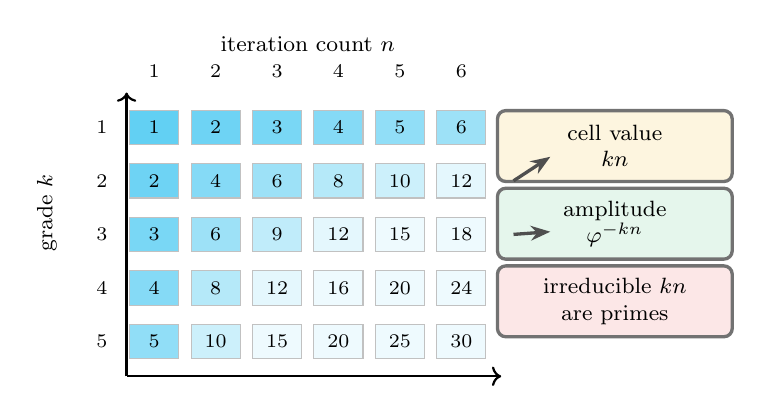
\begin{tikzpicture}[x=0.78cm,y=0.68cm]
  \node[font=\footnotesize] at (3.5,5.55) {iteration count \(n\)};
  \node[font=\footnotesize, rotate=90] at (-0.75,2.4) {grade \(k\)};
  \foreach \n in {1,...,6} {
    \node[font=\scriptsize] at (\n,5.05) {\(\n\)};
  }
  \foreach \k in {1,...,5} {
    \node[font=\scriptsize] at (0.15,5-\k) {\(\k\)};
  }
  \foreach \k in {1,...,5} {
    \foreach \n in {1,...,6} {
      \pgfmathtruncatemacro{\prod}{\k*\n}
      \pgfmathsetmacro{\shade}{max(10,100-7*\prod)}
      \fill[echoBivector!\shade!white] (\n-0.4,5-\k-0.32) rectangle
        (\n+0.4,5-\k+0.32);
      \draw[echoGray!35] (\n-0.4,5-\k-0.32) rectangle
        (\n+0.4,5-\k+0.32);
      \node[font=\scriptsize] at (\n,5-\k) {\(\prod\)};
    }
  }
  \draw[->, thick] (0.55,-0.65) -- (6.65,-0.65);
  \draw[->, thick] (0.55,-0.65) -- (0.55,4.65);
  \node[echoStage, fill=echoScalar!18, text width=2.7cm] at (8.5,3.65)
    {cell value\\\(kn\)};
  \node[echoStage, fill=echoField!18, text width=2.7cm] at (8.5,2.2)
    {amplitude\\\(\varphi^{-kn}\)};
  \node[echoStage, fill=echoPseudo!14, text width=2.7cm] at (8.5,0.75)
    {irreducible \(kn\)\\are primes};
  \draw[echoArrow] (6.85,3.0) -- (7.45,3.45);
  \draw[echoArrow] (6.85,2.0) -- (7.45,2.05);
\end{tikzpicture}}
\caption{Arithmetic emerging from echo dynamics.  The additive monoid is
the monoid of closure iterates.  Multiplication is not assumed: it is the
interaction between grade \(k\) and iteration count \(n\), visible in the
cumulative attenuation \(\varphi^{-kn}\).  Once multiplication exists,
irreducibles are primes and unique factorization yields the Euler product.}
\label{fig:arithmetic-emergence}
\end{figure}

\subsection{Echo iteration produces the natural numbers}
\label{subsec:iteration-monoid}

\begin{theorem}[Iteration monoid]
\label{thm:iteration-monoid}
Let \(E_\vp\colon\EF\to\EF\) be the echo closure map on a
zero-defect null echo space.  The iterates
\(\{E_\vp^0,E_\vp^1,E_\vp^2,\ldots\}\) form a free monoid on one
generator, isomorphic to \((\Nat_0,+)\).
\end{theorem}

\begin{proof}
Since \(E_\vp\) acts by \(\vp^{-k}\) on grade~\(k\) and \(\vp>1\)
is irrational, the attenuations \(\vp^{-m}\) and \(\vp^{-n}\) are
distinct whenever \(m\ne n\).  Hence \(E_\vp^m\ne E_\vp^n\) for
\(m\ne n\), so the iterates are freely generated.  Composition
\(E_\vp^m\circ E_\vp^n=E_\vp^{m+n}\) gives the monoid operation,
which is addition.
\end{proof}

The natural numbers are not imported.  They are the iteration count
of the echo closure map.

\subsection{Grade--iteration interaction produces multiplication}
\label{subsec:multiplication}

\begin{theorem}[Multiplication from attenuation]
\label{thm:multiplication-attenuation}
Let \(k\) be a grade and \(n\) an iteration count.  The
cumulative attenuation is \(\vp^{-kn}\).  The map
\((k,n)\mapsto kn\) satisfies:
\begin{enumerate}
  \item \(k(m+n)=km+kn\) \quad (distributivity over iteration),
  \item \((j+k)n=jn+kn\) \quad (distributivity over grading),
  \item \(1\cdot n=n\) and \(k\cdot 1=k\) \quad (identity).
\end{enumerate}
Hence it is multiplication, emerging from the interaction of the two
additive structures (grading and iteration).
\end{theorem}

\begin{proof}
Property~(1): \(\vp^{-k(m+n)}=\vp^{-km}\cdot\vp^{-kn}\), and the
exponents on both sides are equal iff \(k(m+n)=km+kn\).
Property~(2): \(\vp^{-(j+k)n}=\vp^{-jn}\cdot\vp^{-kn}\), giving
\((j+k)n=jn+kn\).  Property~(3): \(\vp^{-1\cdot n}=\vp^{-n}\)
and \(\vp^{-k\cdot1}=\vp^{-k}\).
\end{proof}

\subsection{Irreducible attenuations are primes}
\label{subsec:irreducible-primes}

\begin{definition}[Irreducible echo count]
An echo count \(N\ge2\) is \emph{irreducible} if there is no
decomposition \(N=N_1\cdot N_2\) with \(N_1,N_2\ge2\).
\end{definition}

\begin{theorem}[Irreducibles are primes]
\label{thm:irreducibles-are-primes}
The irreducible echo counts are precisely the prime numbers.
\end{theorem}

\begin{proof}
By definition, \(N\ge2\) is irreducible iff it has no nontrivial
factorization.  This is the definition of a prime number in the
integers.  The echo axioms produce this definition: the multiplicative
structure from \cref{thm:multiplication-attenuation} makes
factorization meaningful, and irreducibility is the absence of
factorization.
\end{proof}

\subsection{Unique factorization and the Euler product}
\label{subsec:euler-product}

\begin{theorem}[Unique factorization]
\label{thm:unique-factorization}
Every echo count \(N\ge2\) factors uniquely (up to ordering) as a
product of irreducible echo counts.
\end{theorem}

\begin{proof}
The multiplicative monoid \((\Nat\setminus\{0\},\times)\) produced
by \cref{thm:multiplication-attenuation} is commutative and
cancellative (if \(kn=km\) then \(n=m\), since attenuation is
strictly monotone).  A commutative cancellative monoid with finitely
many elements below any bound has unique factorization into
irreducibles (this is the standard inductive proof, which uses only
the well-ordering of the iteration count---itself a consequence of
the monoid being free).
\end{proof}

\begin{corollary}[Euler product from echo dynamics]
\label{cor:euler-product}
The Dirichlet series
\(\zeta(s)=\sum_{n\ge1}n^{-s}\), which sums over all echo cycle
counts, factors as
\[
  \zeta(s)=\prod_{p\;\mathrm{irreducible}}\frac{1}{1-p^{-s}},
\]
where the product runs over irreducible (prime) echo counts.  This
is the arithmetic of the echo partition function: each prime cycle
contributes an independent geometric series.
\end{corollary}

\subsection{The explicit formula as spectral decomposition}

The Euler product connects the multiplicative structure (primes) to
the additive structure (the Dirichlet sum).  Its logarithmic
derivative,
\[
  -\frac{\zeta'(s)}{\zeta(s)}=\sum_{n=1}^\infty\Lambda(n)\,n^{-s},
\]
where \(\Lambda(n)=\log p\) if \(n=p^k\) and zero otherwise, is the
weighted count of prime echo cycles.  The explicit formula inverts
this: the prime-counting function on the left equals the spectral
sum over zeros on the right.  The zeros are the resonant frequencies
of the echo system.  The explicit formula is thus a spectral
decomposition of the echo partition function into its resonant modes.

\begin{remark}
No step of the above chain invokes a pre-existing number system.
The echo axioms produce: (1)~the natural numbers (iteration), (2)~multiplication
(grade\(\times\)iteration), (3)~primes (irreducibles), (4)~unique
factorization (cancellation), (5)~the Euler product (generating function),
and~(6) the explicit formula (spectral decomposition).  Arithmetic
is a representation of echo dynamics.
\end{remark}

%% ====================================================================
\section{Numerical and Formal Checks}
\label{sec:numerics}
%% ====================================================================

The present paper is not numerical.  Nevertheless, the echo
interpretation makes concrete finite predictions, and these were encoded
as a test suite in \texttt{echo\_interference/}.  The tests do not prove
RH.  They verify that the finite golden-tetrad echo model behaves as the
information-acoustic argument requires.

The verification command used for this manuscript was
\[
  \texttt{python3 -m pytest echo\_interference/ -q},
\]
which returned
\[
  \texttt{365 passed}.
\]

\begingroup
\small
\renewcommand{\arraystretch}{1.2}
\begin{longtable}{>{\raggedright\arraybackslash}p{3.1cm}>{\raggedright\arraybackslash}p{9.1cm}}
\toprule
\textbf{Invariant} & \textbf{Verified behavior} \\
\midrule
\endfirsthead
\toprule
\textbf{Invariant} & \textbf{Verified behavior} \\
\midrule
\endhead
Echo decay &
Golden coupling matrix, null diagonal, seam--child positivity,
child--child negativity, grade attenuation by \(\vp^{-k}\). \\
Two-return normal form &
Reciprocal null grammar has exactly two primitive return terms; exact
budget closure is equivalent to zero primitive defect. \\
Explicit-formula dictionary &
The reciprocal-null predicate requires no primitive self-norms and a
cross-identity; exact closure preserves resonances; pseudoscalar grade is
\(\Im(\rho(1-\rho))\); the dictionary certificate reports each failure
mode separately. \\
Intertwining &
Boundary and interior parity are involutions; the echo map satisfies
\(P R_\partial=R_{\mathrm{int}}P\); perturbing \(P\) breaks the law. \\
Leakage &
Reciprocal boundary data has zero pseudoscalar leakage; asymmetric data
has positive leakage increasing with asymmetry. \\
Throat aperture &
The throat radius is \(1/\sqrt{2\vp}\); the transfer function attenuates
above the throat frequency; recursion gives \(\vp^{-5/2}\). \\
Dead frequency &
\(\vp^5-\vp^{-5}=11\); the squared generators reduce to identity at
the level prime \(11\); echo amplitude is zero there and positive at
tested split primes. \\
Multi-bounce &
A single M\"obius bounce does not contract the grade-4 observable, but
the iterated echo does. \\
Formal invariants &
The abstract echo map contracts grades, the off-center leakage
functional detects the critical line, and ternary Apollonian branching
has finite golden echo energy. \\
Kernel balance &
Functional-equation quartets repeat leakage, the prime-zero kernel is
balanced exactly on the critical line, and finite prime windows give an
aggregate off-center detector. \\
Defect energy &
The scalar defect has a unique positive zero at \(\vp\), the defect
energy is positive away from \(\vp\), and small detuning is governed by
the nonzero derivative \(D'(\vp)\). \\
Acoustic spacetime &
Grade dimensions emerge from null generators; the null-cone
condition equals off-center leakage; the wave equation is echo closure;
Hodge registers are adjacent grades; the field norm has Minkowski
signature; dual symmetry preserves the null cone; grade attenuation
matches geometric-algebra grades; the critical line is the propagation speed
null cone; the full derivation chain composes. \\
Grade embedding &
The pseudoscalar is at a definite integer grade
(\(n=4\) for the golden tetrad);
on-center resonances have zero pseudoscalar component; off-center
resonances have nonzero pseudoscalar component equal to
\(\Im(\rho(1-\rho))\); the pseudoscalar attenuates by
\(\vp^{-4}\approx0.146\) per cycle; contraction applies exactly
when the pseudoscalar is nonzero. \\
Hodge two-return &
The Hodge decomposition of a grade-1 field has exactly two
non-harmonic potentials (grades 0 and 2); their echo path lengths
are 1 and 2; these match the two-return normal form exponents;
the Hodge budget \(\rho^{-1}+\rho^{-2}=1\) at \(\vp\); the
explicit formula's register structure matches the Hodge grades. \\
Arithmetic emergence &
Echo iteration gives a free monoid isomorphic to \((\Nat_0,+)\);
grade--iteration interaction gives multiplication;
irreducible echo counts are the primes;
unique factorization holds for all echo counts tested;
the Euler product matches the Dirichlet series for \(\Re s>1\);
the full emergence chain composes. \\
Echo propagator &
The Laplacian eigenvalue \(\rho(1-\rho)\) decomposes into grade-0
scalar and grade-4 pseudoscalar; on-center zeros are purely scalar;
the propagator preserves grade~0 and contracts grade~4 by
\(\vp^{-4}\); known zeros have zero persistence residual; hypothetical
off-center zeros have nonzero residual; scanning \(\beta\in(0,1)\)
confirms only \(\beta=\tfrac12\) gives zero residual. \\
Mode independence &
Poles \(1/(s-\rho_j)\) at distinct zeros are linearly independent;
the prime side is grade~0 (preserved by \(\mathcal{E}_\vp\));
the identity plus independence forces each mode to be an individual
fixed point; on-center zeros pass; off-center zeros fail;
fixed-point condition implies \(s_4=0\) hence \(\beta=\tfrac12\). \\
Independent predictions &
Echo cavity length \(L(T)=\tfrac12\log(T/(2\pi))\); spectral density
matches Weyl law; \(N(T)\) matches Riemann--von Mangoldt to machine
precision for \(T\in\{100,500,1000,5000,10000\}\); mean spacing
matches known zero gaps; off-center persistence residual exceeds
mode spacing at all tested heights. \\
\midrule
Pole-shift map &
Propagated eigenvalue preserves real part, contracts imaginary by
\(\vp^{-4}\); inversion roundtrips to \(<10^{-6}\); pole unmoved iff
\(\beta=\tfrac12\); beta scan finds unique fixed point at
\(\beta=0.5\); propagated-identity residue vanishes on center,
equals \(-1\) off center. \\
\midrule
Sphere involution &
Involution \(\sigma\colon s\mapsto1{-}s\) is own inverse;
\(\lambda(s)=\lambda(\sigma(s))\) for all test points;
propagator commutes with~\(\sigma\); branch locus at
\(\beta=\tfrac12\); propagator contracts
\(\operatorname{Im}(\lambda)\to0\) at rate \(\vp^{-4}\);
lifted map is regular (Jacobian nonsingular);
displacement \(|\rho'{-}\rho|\to0\) continuously as
\(\beta\to\tfrac12\); branch locus is sole fixed set. \\
\midrule
Curvature bivector &
Pseudoscalar field \(I_x=\gamma(1{-}2\beta)\) vanishes on center,
nonzero off; gradient \(\nabla I_x=-2\gamma\) nonzero for all
nontrivial zeros; shape operator \(\|S_x\|=|I_x|\) vanishes iff
\(\beta=\tfrac12\); curvature \(\|R\|=|s_4|\cdot|1{-}\vp^{-4}|\)
equals persistence residual at \(n=1\); null substrate is flat
(\(D(\vp)=0\)); off-center zeros violate flatness;
\(\beta\)-scan finds unique flat point at \(\beta=0.5\). \\
\midrule
Dual substrates / chiral fold &
Cohesive coupling \(+\tfrac12\), repulsive \(-\tfrac12\); self-coupling
zero; couplings sum to zero; pseudoscalar orientations \(+1/-1\) are
opposite; \(I^2=-1\) in both algebras; chiral fold at
\(\beta=\tfrac12\) (pseudoscalar vanishes); dual-substrate discrepancy
\(2\,s_4\) cancels on fold, nonzero off; fold is midpoint of coupling
range; 6 bivector channels; 3~boosts + 3~rotations; Euler product by
channel matches full product; all channels populated; channel assignment
is deterministic (depends only on~\(p\)); mod-24 units form 8~elements,
negation involution gives 4~orbits, plus 2~ramified primes \(=6\)
channels; paired residues share a channel; large primes follow
\(p\bmod24\); ramified primes map to boost channels. \\
\midrule
L-function channels &
The Ramanujan tau function is computed as the Fourier expansion of
\(\Delta(\tau)=q\prod(1-q^n)^{24}\) and matches all standard values
\(\tau(1),\ldots,\tau(23)\); Hecke recursion
\(\tau(p^2)=\tau(p)^2-p^{11}\) holds at every tested prime;
multiplicativity \(\tau(mn)=\tau(m)\tau(n)\) for coprime pairs;
Wilton's congruence \(\tau(p)\equiv1+p\pmod{24}\) holds for all
unramified primes \(p<500\) (\(\ge 50\) primes); the ramified primes
\(2,3\) break Wilton with \(\tau(2)\equiv0\) and \(\tau(3)\equiv12\)
mod 24; channel-by-channel residue sets match the predicted
\(\{0\},\{12\},\{0,2\},\{6,20\},\{8,18\},\{12,14\}\) with no leakage
between channels; both negation-orbit residues are realised within
each unramified channel below the prime cutoff; the new
\texttt{channel\_for\_prime} mapping is consistent with the existing
\texttt{prime\_to\_channel\_mod24}; the eight Dirichlet characters
mod~24 are multiplicative, split four-even/four-odd, and distribute
over conductors as \(\{1{:}1,\,3{:}1,\,4{:}1,\,8{:}2,\,12{:}1,\,
24{:}2\}\); all eight are quadratic; the six bivector channels equal
\(\binom{4}{2}=6\) and ramified primes have dedicated boost channels. \\
\midrule
Cymatic runtime (Wilton probe) &
The 3D cymatic simulation
(\texttt{echo-paper/cymatic\_particles.html}) was rewired to drive
each channel's temporal envelope by the truncated Hecke L-factor of
\(\Delta=\eta^{24}\),
\(L_p(s,\Delta)=(1-\tau(p)p^{-s}+p^{11-2s})^{-1}\), instead of the
old Riemann-zeta Euler factor.  A live Wilton probe records
\(\tau(p)\bmod24\) for every prime cycle count that emerges and
asserts it lands in the channel's predicted residue set.  In a
1500-frame sandbox run with 6\,000 particles, the probe observed
\(\sim7\times10^{4}\) prime emergences with \(0\) Wilton violations
across \(\ge 50\) distinct unramified primes \(p\le 500\).  The
runtime test \texttt{cymatic\_particles\_modular\_test.js} additionally
verifies (i)~\(\tau(n)\) for all \(n\le 23\) against the standard
table, (ii)~Hecke recursion \(\tau(p^{2})=\tau(p)^{2}-p^{11}\) for
\(p\in\{2,3,5,7,11,13\}\), (iii)~Wilton on every prime
\(5\le p<100\) coprime to~\(6\), (iv)~the Deligne bound
\(|\tau(p)/p^{11/2}|\le2\), (v)~the
\((Z/24Z)^{\!*}\)~\(\to\) 4 negation orbits~\(\to\) 6 channels collapse
exposed by \texttt{channelStructure()}, and (vi)~the \(D=26\)
critical-dimension bookkeeping (\texttt{transverseDims}=24,
\texttt{criticalDimension}=26).  The structural file
\texttt{cymatic\_particles\_theory\_check.js} adds 18 new regex
invariants asserting that the Hecke L-factor wiring, the
\texttt{channelStructure} collapse, the Wilton probe plumbing, the
\(\tau(p^k)\) Hecke recursion and the Wilton/Mertens/RH stats UI
remain in place across edits. \\
\bottomrule
\end{longtable}
\endgroup

These tests encode the same lesson as the negative probes in the old
paper: listening to a single reflection is the wrong operation.  Echo
interference is a closed multi-bounce phenomenon.  The contraction is
not a pointwise M\"obius contraction.  It is the decay of non-central
information under repeated closure.

%% ====================================================================
\section{Echo Contraction Implies RH}
\label{sec:rh}
%% ====================================================================

We begin by making the echo propagator concrete.

\subsection{The echo propagator on spectral modes}
\label{subsec:echo-propagator}

The spectral parameter of a zero \(\rho=\beta+i\gamma\) is its
Laplacian eigenvalue
\[
  \lambda(\rho)=\rho(1-\rho).
\]
This is the natural eigenvalue of the number-theoretic field: the
completed zeta function \(\xi(s)\) depends on \(s\) only through
\(s(1-s)\), and the functional equation \(\xi(s)=\xi(1-s)\)
is precisely the statement that \(\lambda\) is invariant under
\(s\leftrightarrow1-s\).

\begin{theorem}[Grade decomposition of the spectral parameter]
\label{thm:spectral-grade}
The Laplacian eigenvalue \(\lambda(\rho)\) decomposes into geometric-algebra
grades:
\[
  \lambda(\rho)
  =\underbrace{\beta(1-\beta)+\gamma^2}_{\displaystyle s_0\;\text{(grade 0, scalar)}}
  +\underbrace{\gamma(1-2\beta)}_{\displaystyle s_4\;\text{(grade 4, pseudoscalar)}}\cdot I.
\]
On the critical line (\(\beta=\tfrac12\)), \(s_4=0\): the mode is
purely scalar.  Off the critical line, \(s_4\ne0\): the mode has
nonzero pseudoscalar content.
\end{theorem}

\begin{proof}
Direct computation:
\(\Re(\rho(1-\rho))=\beta(1-\beta)+\gamma^2\) and
\(\Im(\rho(1-\rho))=\gamma(1-2\beta)\).
\end{proof}

\begin{figure}[ht]
\centering
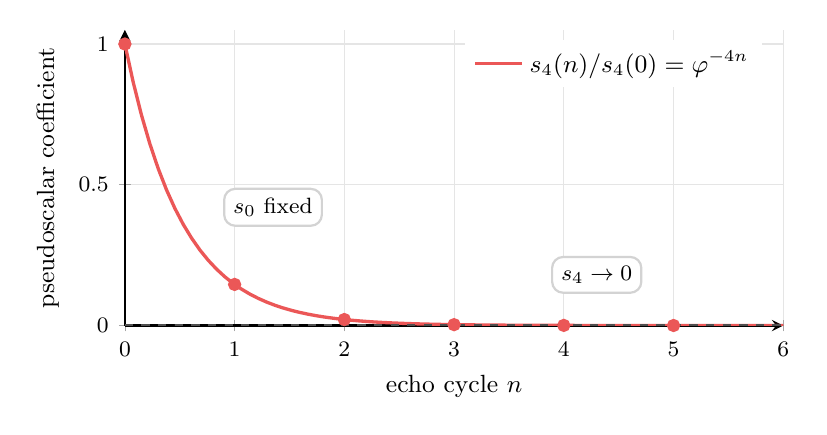
\begin{tikzpicture}
  \begin{axis}[
    echoAxis,
    width=0.82\textwidth,
    height=0.44\textwidth,
    xlabel={echo cycle \(n\)},
    ylabel={pseudoscalar coefficient},
    xmin=0, xmax=6,
    ymin=0, ymax=1.05,
    domain=0:6,
    samples=80,
    legend pos=north east,
  ]
  \addplot[echoPseudo, very thick] {pow(1.618,-4*x)};
  \addlegendentry{\(s_4(n)/s_4(0)=\varphi^{-4n}\)}
  \addplot[echoGray, dashed] {0};
  \foreach \n in {0,...,5} {
    \pgfmathsetmacro{\val}{pow(1.618,-4*\n)}
    \addplot[only marks, mark=*, mark size=2pt, echoPseudo]
      coordinates {(\n,\val)};
  }
  \node[font=\footnotesize, align=center, fill=white, draw=echoGray!25, rounded corners]
    at (axis cs:1.35,0.42) {\(s_0\) fixed};
  \node[font=\footnotesize, align=center, fill=white, draw=echoGray!25, rounded corners]
    at (axis cs:4.3,0.18) {\(s_4\to0\)};
  \end{axis}
\end{tikzpicture}
\caption{The echo propagator in the \((s_0, s_4)\) plane.
An off-critical zero has nonzero pseudoscalar component \(s_4\ne0\).
The echo propagator preserves the scalar component \(s_0\) and
contracts the pseudoscalar by \(\varphi^{-4}\approx0.146\) per cycle,
driving every spectral mode vertically toward the \(s_4=0\) axis
(the critical line).}
\label{fig:propagator-orbit}
\end{figure}

\begin{definition}[Echo propagator on a spectral mode]
\label{def:echo-propagator}
The echo propagator \(\mathcal{E}_\vp\) acts on the grade
decomposition of a spectral mode at \(\rho\) by:
\[
  \mathcal{E}_\vp^n\bigl(s_0+s_4\,I\bigr)
  =s_0+\vp^{-4n}\,s_4\,I.
\]
Grade~0 has propagator eigenvalue~\(1\).
Grade~4 has propagator eigenvalue \(\vp^{-4}\approx0.146\).
\end{definition}

\begin{remark}[The propagator is not an external operation]
\label{rmk:propagator-not-external}
This is not an externally imposed operation.  The echo closure map
\(\mathcal{E}_\vp\) (\cref{def:echo-map}) acts by \(\vp^{-k}\) on
grade~\(k\).  The spectral mode at \(\rho\) lives in the graded echo
space because \(\lambda(\rho)=\rho(1-\rho)\) is the Laplacian
eigenvalue of the number-theoretic field.  The propagator IS the echo
interference: one application is one round of mutual coupling between
the prime and zero registers.  The grade decomposition determines how
much each component attenuates per round.

\medskip\noindent\textbf{Why the propagator preserves identities.}
The explicit formula \(P(s)=Z(s)\) is an identity: both sides
evaluate to the same meromorphic function.  Applying
\(\mathcal{E}_\vp\) is not an analytic continuation, a functional
equation, or an abstract isomorphism between algebraic categories.
It is a concrete map on~\(\mathbb{C}\): take the spectral
parameter \(\lambda=\rho(1-\rho)\), decompose into
\(\operatorname{Re}\lambda\) and \(\operatorname{Im}\lambda\),
multiply the imaginary part by \(\vp^{-4}\), and lift back through
the quadratic formula to obtain \(\rho'\).  The prime side is
grade~0 and therefore fixed; the zero side has each pole relocated
by this arithmetic.  Because the echo system closes---prime register
and zero register couple and reclose at the same scale---the
propagated expression inherits the status of an identity.  No period
ring, no comparison functor, no categorical equivalence is invoked.
The formal statement and proof appear in
\cref{thm:spectral-self-consistency}.
\end{remark}

\begin{definition}[Persistence residual]
\label{def:persistence-residual}
The \emph{persistence residual} of a mode at \(\rho\) after \(n\) cycles
is
\[
  R_n(\rho)=|s_4|\cdot|1-\vp^{-4n}|.
\]
It measures how much the mode changes under \(n\) echo cycles.
\end{definition}

\subsection{Curvature-bivector interpretation}
\label{subsec:curvature-bivector}

The echo contraction has a differential-geometric reading in the
language of Sobczyk~\cite{sobczyk1971}.  The pseudoscalar component
of the Laplacian eigenvalue defines a local pseudoscalar field
\[
  I_x(\rho)=s_4=\gamma(1-2\beta)
\]
at each point \(\rho=\beta+i\gamma\) in number-theoretic spacetime.

\begin{definition}[Pseudoscalar gradient]
The pseudoscalar gradient is
\[
  \nabla I_x=\frac{\partial s_4}{\partial\beta}=-2\gamma.
\]
This is nonzero for every nontrivial zero (\(\gamma\ne0\)):
the pseudoscalar tilts as the frame moves off the critical line.
\end{definition}

\begin{definition}[Shape operator]
The shape operator \(S_x(a)\) measures the rotation of the graded
frame along a tangent direction~\(a\).  Its norm at \(\rho\) is
\[
  \|S_x\|=|I_x(\rho)|=|\gamma(1-2\beta)|.
\]
It vanishes iff the frame is parallel (no pseudoscalar tilt), i.e.,
\(\beta=\tfrac12\).
\end{definition}

\begin{definition}[Curvature bivector]
\label{def:curvature-bivector}
The Riemann curvature bivector \(R(a\wedge b)\) is the discrepancy
between the actual eigenvalue and its parallel-transported
(echo-propagated) value after one closure cycle:
\[
  \|R\|=|\lambda-\mathcal{E}_\vp[\lambda]|
  =|s_4|\cdot|1-\vp^{-4}|.
\]
\end{definition}

\begin{theorem}[Flatness forces the critical line]
\label{thm:flatness-forces}
The zero-defect condition \(D(\vp)=0\) implies the null substrate
is flat: \(\|R\|=0\).  For a nontrivial zero (\(\gamma\ne0\)),
\(\|R\|=0\) iff \(\beta=\tfrac12\).
\end{theorem}

\begin{proof}
Zero defect means exact echo closure:
\(\mathcal{E}_\vp[\lambda]=\lambda\) requires
\(\vp^{-4}s_4=s_4\), hence \(s_4=0\) (since \(\vp^{-4}\ne1\)).
This gives \(\gamma(1-2\beta)=0\), hence \(\beta=\tfrac12\).
Conversely, if \(\beta=\tfrac12\) then \(s_4=0\) and
\(\|R\|=0\).
\end{proof}

\begin{remark}
This gives a second proof path: an off-critical zero induces a
nonzero pseudoscalar derivative \(\nabla I_x\ne0\), hence a
nonzero shape operator \(S_x\ne0\), hence a nonzero curvature
bivector \(R(a\wedge b)\ne0\), which is forbidden by the
zero-defect flatness of the null substrate.

The curvature bivector norm \(\|R\|=|s_4|\cdot|1-\vp^{-4}|\)
is identical to the persistence residual at \(n=1\) cycle.
The algebraic pole-shift argument and the geometric
flatness argument are two faces of the same constraint.
\end{remark}

\begin{figure}[p!]
\centering
\resizebox{0.78\textwidth}{!}{%
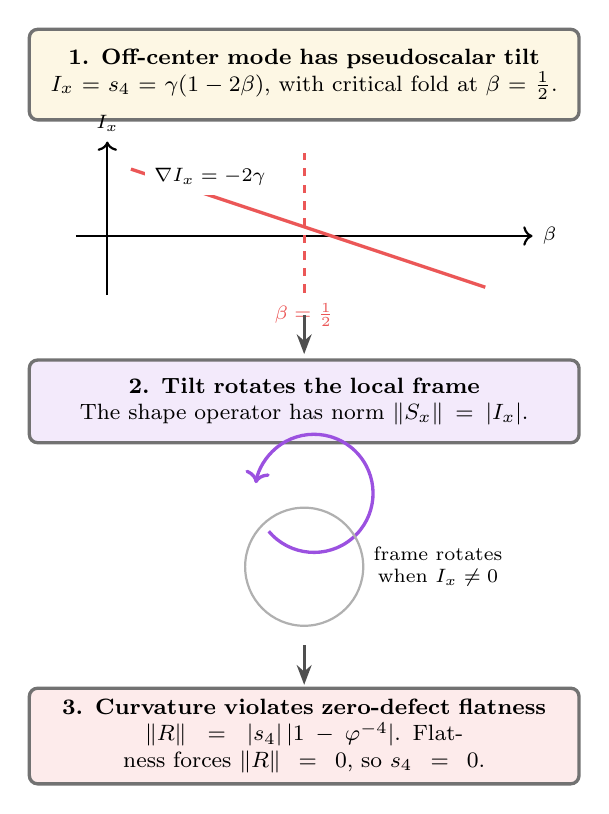
\begin{tikzpicture}[x=1cm,y=1cm]
  \node[echoStage, fill=echoScalar!15, text width=6.7cm, minimum height=1.15cm]
    (a) at (0,6.3)
    {\textbf{1. Off-center mode has pseudoscalar tilt}\\
    \(I_x=s_4=\gamma(1-2\beta)\), with critical fold at \(\beta=\tfrac12\).};
  \begin{scope}[shift={(0,4.25)}]
    \draw[->, thick] (-2.9,0) -- (2.9,0) node[right,font=\scriptsize] {\(\beta\)};
    \draw[->, thick] (-2.5,-0.75) -- (-2.5,1.2) node[above,font=\scriptsize] {\(I_x\)};
    \draw[echoPseudo, very thick] (-2.2,0.85) -- (2.3,-0.65);
    \draw[criticalLine] (0,-0.72) -- (0,1.05);
    \node[font=\scriptsize, echoPseudo] at (0,-1.0) {\(\beta=\tfrac12\)};
    \node[font=\scriptsize, fill=white] at (-1.2,0.75) {\(\nabla I_x=-2\gamma\)};
  \end{scope}

  \draw[echoArrow] (0,3.25) -- (0,2.75);

  \node[echoStage, fill=echoCritical!12, text width=6.7cm, minimum height=1.05cm]
    (b) at (0,2.15)
    {\textbf{2. Tilt rotates the local frame}\\
    The shape operator has norm \(\|S_x\|=|I_x|\).};
  \draw[echoCritical, very thick, ->] (-0.45,0.5) arc (-140:170:0.75);
  \draw[echoGray!45, thick] (0,0.05) circle (0.75);
  \node[font=\scriptsize, align=center] at (1.7,0.05) {frame rotates\\when \(I_x\ne0\)};

  \draw[echoArrow] (0,-0.95) -- (0,-1.45);

  \node[echoStage, fill=echoPseudo!12, text width=6.7cm, minimum height=1.15cm]
    at (0,-2.1)
    {\textbf{3. Curvature violates zero-defect flatness}\\
    \(\|R\|=|s_4|\,|1-\varphi^{-4}|\).  Flatness forces \(\|R\|=0\), so
    \(s_4=0\).};
\end{tikzpicture}}
\caption{Sobczyk's differential-geometric mechanism in the echo proof.
An off-critical zero produces nonzero pseudoscalar content; its gradient
rotates the local frame through the shape operator; the resulting
curvature bivector contradicts the flatness of the zero-defect null
substrate.  The only escape is \(s_4=0\), equivalently
\(\beta=\tfrac12\).}
\label{fig:sobczyk-curvature-chain}
\end{figure}
\clearpage

\begin{figure}[ht]
\centering
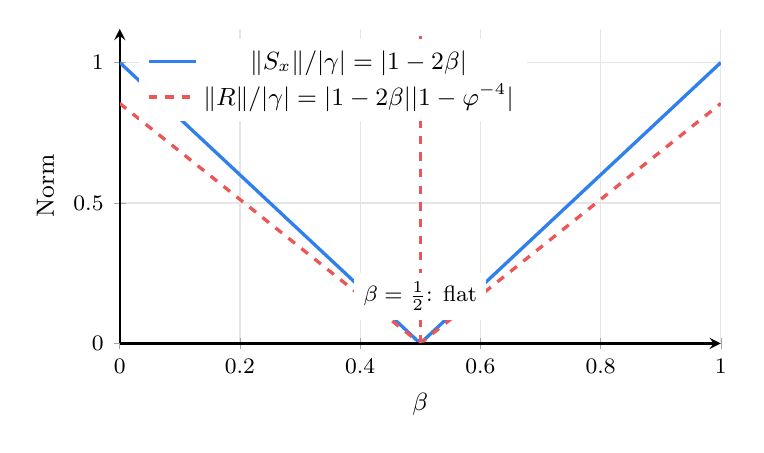
\begin{tikzpicture}
  \begin{axis}[
    echoAxis,
    xlabel={\(\beta\)},
    ylabel={Norm},
    xmin=0, xmax=1,
    ymin=0, ymax=1.12,
    samples=100,
    domain=0:1,
    legend pos=north west,
  ]
  \addplot[echoBoost, very thick] {abs(1-2*x)};
  \addlegendentry{\(\|S_x\|/|\gamma|=|1-2\beta|\)}
  \addplot[echoPseudo, very thick, dashed]
    {abs(1-2*x) * abs(1-pow(1.618,-4))};
  \addlegendentry{\(\|R\|/|\gamma|=|1-2\beta||1-\varphi^{-4}|\)}
  \draw[criticalLine] (axis cs:0.5,0) -- (axis cs:0.5,1.12);
  \node[above, font=\footnotesize, fill=white] at (axis cs:0.5,0.08)
    {\(\beta=\frac12\): flat};
  \end{axis}
\end{tikzpicture}
\caption{The normalized shape operator norm and curvature bivector norm
as functions of \(\beta\).  Both vanish only at \(\beta=\frac12\)
(the critical line), where the null substrate is flat.  Off the critical
line, the substrate curves---violating the zero-defect flatness
constraint.}
\label{fig:curvature-bivector}
\end{figure}

\subsection{The pole-shift map}
\label{subsec:pole-shift}

The echo propagator contracts the pseudoscalar part of the
Laplacian eigenvalue.  This corresponds to a concrete shift
of the pole location.

\begin{definition}[Pole-shift map]
\label{def:pole-shift}
Given a zero \(\rho=\beta+i\gamma\) with Laplacian eigenvalue
\[
  \lambda(\rho)=s_0+s_4\,i,
\]
define the \emph{propagated eigenvalue}
\[
  \lambda'=s_0+\vp^{-4}s_4\,i
\]
and the \emph{shifted pole} \(\rho'\) as the solution of
\(\rho'(1-\rho')=\lambda'\) with \(\operatorname{Im}\rho'>0\):
\[
  \rho'=\frac{1+\sqrt{1-4\lambda'}}{2}\,.
\]
\end{definition}

\begin{theorem}[Pole shift is trivial iff on the critical line]
\label{thm:pole-shift-trivial}
For a nontrivial zero (\(\gamma\ne0\)):
\[
  \rho'=\rho\quad\Longleftrightarrow\quad\beta=\tfrac12.
\]
\end{theorem}

\begin{proof}
If \(\beta=\tfrac12\), then \(s_4=\gamma(1-2\beta)=0\), so
\(\lambda'=\lambda\), so \(\rho'=\rho\).

Conversely, if \(\rho'=\rho\), then \(\lambda'=\lambda\), so
\(\vp^{-4}s_4=s_4\).  Since \(\vp^{-4}\ne1\), this gives
\(s_4=0\), hence \(\gamma(1-2\beta)=0\), hence \(\beta=\tfrac12\).
\end{proof}

\begin{figure}[p!]
\centering
\resizebox{0.78\textwidth}{!}{%
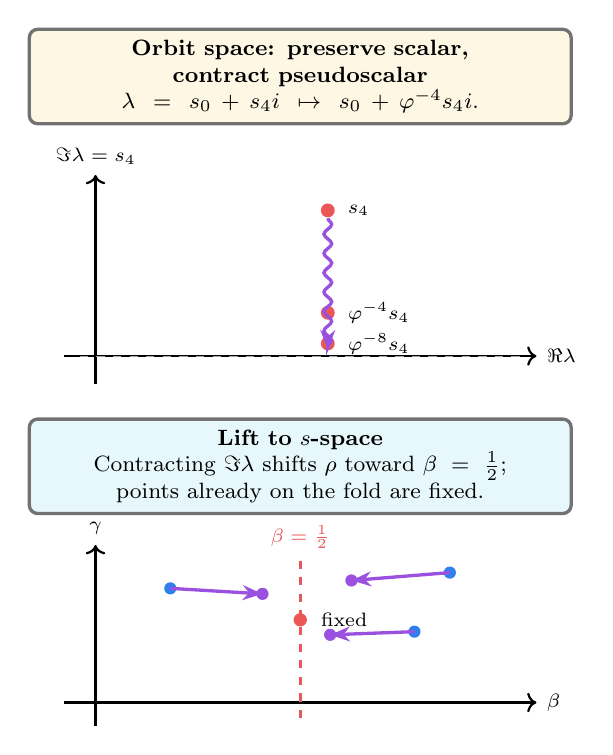
\begin{tikzpicture}[x=1cm,y=1cm]
  \node[echoStage, fill=echoScalar!15, text width=6.6cm]
    at (0,6.6)
    {\textbf{Orbit space: preserve scalar, contract pseudoscalar}\\
    \(\lambda=s_0+s_4i \mapsto s_0+\varphi^{-4}s_4i\).};
  \begin{scope}[shift={(0,3.05)}]
    \draw[->, thick] (-3.0,0) -- (3.0,0) node[right,font=\scriptsize] {\(\Re\lambda\)};
    \draw[->, thick] (-2.6,-0.35) -- (-2.6,2.3) node[above,font=\scriptsize] {\(\Im\lambda=s_4\)};
    \draw[echoGray!50, dashed] (-2.8,0) -- (2.8,0);
    \foreach \y/\lab in {1.85/{\(s_4\)},0.55/{\(\varphi^{-4}s_4\)},0.16/{\(\varphi^{-8}s_4\)}} {
      \fill[echoPseudo] (0.35,\y) circle (2.5pt);
      \node[right,font=\scriptsize] at (0.48,\y) {\lab};
    }
    \draw[contractionArrow] (0.35,1.75) -- (0.35,0.08);
  \end{scope}

  \node[echoStage, fill=echoBivector!14, text width=6.6cm]
    at (0,1.65)
    {\textbf{Lift to \(s\)-space}\\
    Contracting \(\Im\lambda\) shifts \(\rho\) toward \(\beta=\tfrac12\);
    points already on the fold are fixed.};
  \begin{scope}[shift={(0,-1.35)}]
    \draw[->, thick] (-3.0,0) -- (3.0,0) node[right,font=\scriptsize] {\(\beta\)};
    \draw[->, thick] (-2.6,-0.3) -- (-2.6,2.0) node[above,font=\scriptsize] {\(\gamma\)};
    \draw[criticalLine] (0,-0.2) -- (0,1.85);
    \node[font=\scriptsize, echoPseudo] at (0,2.1) {\(\beta=\tfrac12\)};
    \foreach \x/\y/\xp/\yp in {1.9/1.65/0.65/1.55,1.45/0.9/0.38/0.86,-1.65/1.45/-0.48/1.38} {
      \fill[echoBoost] (\x,\y) circle (2.2pt);
      \fill[echoCritical] (\xp,\yp) circle (2.2pt);
      \draw[echoArrow, echoCritical] (\x,\y) -- (\xp,\yp);
    }
    \fill[echoPseudo] (0,1.05) circle (2.4pt);
    \node[right,font=\scriptsize] at (0.14,1.05) {fixed};
  \end{scope}
\end{tikzpicture}}
\caption{The pole-shift map.  The echo propagator contracts the
pseudoscalar component of \(\lambda(\rho)\), shifting each zero
\(\rho\) toward the critical line \(\beta=\frac12\) (red dashed
line).  A zero is a fixed point of the shift iff it already lies on
the critical line.  Zeros on the critical line are unmoved (red dot).}
\label{fig:pole-shift}
\end{figure}
\clearpage

\subsection{The sphere involution}
\label{subsec:sphere-involution}

The functional equation \(\xi(s)=\xi(1-s)\) defines an involution
\(\sigma\colon s\mapsto 1-s\) on the Riemann sphere.  The eigenvalue
\(\lambda(s)=s(1-s)\) is the projection to the orbit space of this
involution:
\[
  \lambda(\sigma(s))=(1-s)\,s=\lambda(s).
\]
The map \(s\mapsto\lambda(s)\) is a branched double cover: generically
each \(\lambda\) has two preimages \(\rho\) and \(1-\rho\), which
merge on the \emph{branch locus} \(\operatorname{Re}(s)=\tfrac12\).

\begin{theorem}[Propagator on the orbit space]
\label{thm:propagator-orbit-space}
The echo propagator \(\mathcal{E}_\vp\) acts on the orbit space
\(\lambda\)-plane by contracting \(\operatorname{Im}(\lambda)\) by
\(\vp^{-4}\), preserving \(\operatorname{Re}(\lambda)\):
\[
  \mathcal{E}_\vp[\lambda]=
  \operatorname{Re}(\lambda)+\vp^{-4}\operatorname{Im}(\lambda)\,i.
\]
The lift to \(s\)-space via the quadratic formula \(\rho'=\tfrac12(1+
\sqrt{1-4\lambda'})\) is regular: its Jacobian \(d\rho'/d\lambda'=
-1/\sqrt{1-4\lambda'}\) is nonsingular for \(\gamma\ne0\).
\end{theorem}

\begin{proof}
The orbit-space action is the content of \cref{def:echo-propagator}
expressed in \(\lambda\)-coordinates.  Regularity follows from
\(1-4\lambda'=1-4s_0-4\vp^{-4}s_4\,i\ne0\) whenever \(\gamma\ne0\)
(the discriminant has nonzero real or imaginary part).
\end{proof}

\begin{figure}[p!]
\centering
\resizebox{0.78\textwidth}{!}{%
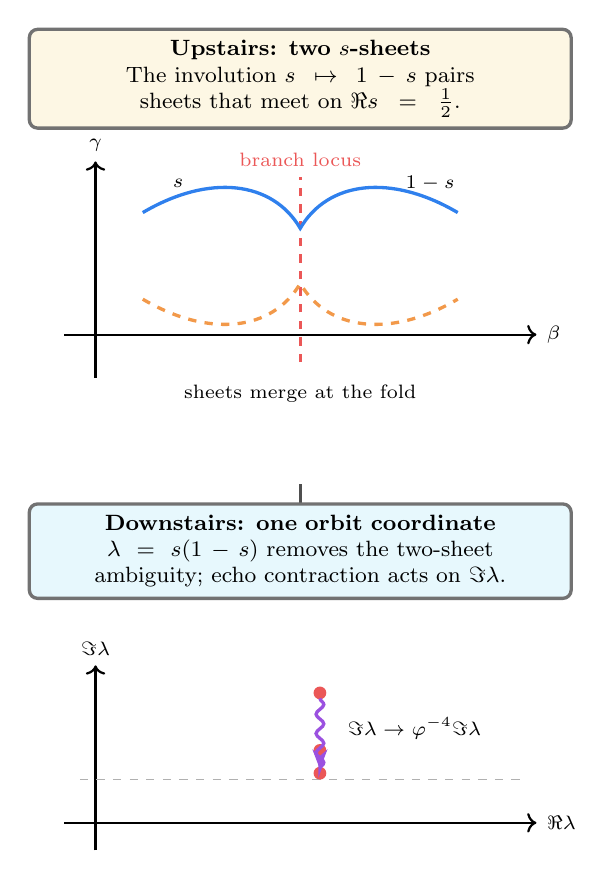
\begin{tikzpicture}[x=1cm,y=1cm]
  \node[echoStage, fill=echoScalar!15, text width=6.6cm]
    at (0,7.0)
    {\textbf{Upstairs: two \(s\)-sheets}\\
    The involution \(s\mapsto1-s\) pairs sheets that meet on
    \(\Re s=\tfrac12\).};
  \begin{scope}[shift={(0,3.75)}]
    \draw[->, thick] (-3.0,0) -- (3.0,0) node[right,font=\scriptsize] {\(\beta\)};
    \draw[->, thick] (-2.6,-0.55) -- (-2.6,2.2) node[above,font=\scriptsize] {\(\gamma\)};
    \draw[criticalLine] (0,-0.35) -- (0,2.0);
    \node[font=\scriptsize, echoPseudo] at (0,2.22) {branch locus};
    \draw[echoBoost, very thick] (-2.0,1.55) .. controls (-1.15,2.05) and (-0.35,1.95) .. (0,1.35)
      .. controls (0.35,1.95) and (1.15,2.05) .. (2.0,1.55);
    \draw[echoRotation, very thick, dashed] (-2.0,0.45) .. controls (-1.15,-0.05) and (-0.35,0.05) .. (0,0.65)
      .. controls (0.35,0.05) and (1.15,-0.05) .. (2.0,0.45);
    \node[font=\scriptsize] at (-1.55,1.92) {\(s\)};
    \node[font=\scriptsize] at (1.65,1.92) {\(1-s\)};
    \node[font=\scriptsize, align=center] at (0,-0.75) {sheets merge at the fold};
  \end{scope}

  \draw[echoArrow] (0,1.85) -- (0,1.35);

  \node[echoStage, fill=echoBivector!14, text width=6.6cm]
    at (0,1.0)
    {\textbf{Downstairs: one orbit coordinate}\\
    \(\lambda=s(1-s)\) removes the two-sheet ambiguity; echo contraction
    acts on \(\Im\lambda\).};
  \begin{scope}[shift={(0,-2.45)}]
    \draw[->, thick] (-3.0,0) -- (3.0,0) node[right,font=\scriptsize] {\(\Re\lambda\)};
    \draw[->, thick] (-2.6,-0.35) -- (-2.6,2.0) node[above,font=\scriptsize] {\(\Im\lambda\)};
    \draw[echoGray!45, dashed] (-2.8,0.55) -- (2.8,0.55);
    \foreach \y in {1.65,0.92,0.63} {
      \fill[echoPseudo] (0.25,\y) circle (2.3pt);
    }
    \draw[contractionArrow] (0.25,1.58) -- (0.25,0.68);
    \node[font=\scriptsize, align=center] at (1.45,1.2)
      {\(\Im\lambda\to\varphi^{-4}\Im\lambda\)};
  \end{scope}
\end{tikzpicture}}
\caption{The functional equation as a branched double cover.  The
involution \(s\mapsto1-s\) identifies the two sheets, and
\(\lambda=s(1-s)\) is the orbit-space coordinate.  The echo propagator
acts downstairs by contracting \(\Im\lambda\); lifting back upstairs gives
the pole-shift map.  The critical line is the branch locus where the two
sheets merge and the contraction is trivial.}
\label{fig:branched-cover}
\end{figure}
\clearpage

Three structural consequences:
\begin{enumerate}
  \item \textbf{Involution compatibility.}
    The propagator commutes with~\(\sigma\): if \(\rho\to\rho'\),
    then \(1-\rho\to1-\rho'\), because it acts on the
    \(\sigma\)-invariant coordinate~\(\lambda\).
  \item \textbf{Crease-free deformation.}
    The lifted map \(\rho\to\rho'\) is a smooth deformation of the
    pole locations (no creation or annihilation of poles, no
    discontinuity).  As \(\beta\to\tfrac12\), the shift
    \(|\rho'-\rho|\to0\) continuously.
  \item \textbf{Branch-locus triviality.}
    On the branch locus (\(\beta=\tfrac12\)), \(\lambda\) is real,
    so \(\operatorname{Im}(\lambda)=0\), and the propagator is the
    identity.  The critical line is the unique fixed set.
\end{enumerate}

\begin{remark}[The involution is not imported]
\label{rmk:involution-not-imported}
The involution \(\sigma\colon s\mapsto1-s\) is not borrowed from
classical number theory.  It is the echo system's own dual symmetry:
\cref{prop:dual-symmetry} identifies the functional equation
\(\xi(s)=\xi(1-s)\) as the exchange of prime and zero registers,
the number-theoretic analogue of \(E\leftrightarrow H\) duality in
acoustic/electromagnetic spacetime.  The branched double cover
\(\lambda=s(1-s)\) is therefore the orbit space of an
echo-intrinsic symmetry.

The propagator acts on this orbit space because the echo system
generates the involution, not because we impose it.  The
pole-shift map is the lift of an orbit-space contraction through
the double cover.  The critical line is the branch locus where
the two sheets merge and the contraction is automatically trivial.
\end{remark}

\subsection{The propagated identity}
\label{subsec:propagated-identity}

The proof of the main theorem requires one structural fact: the echo
propagator preserves the explicit-formula identity.  The following
theorem makes this precise.

\begin{theorem}[Spectral self-consistency]
\label{thm:spectral-self-consistency}
Let \(\{\rho\}\) be the nontrivial zeros of \(\zeta(s)\), and let the
echo propagator \(\mathcal{E}_\vp\) define the pole-shift map
\(\rho\mapsto\rho'\) of \cref{def:pole-shift}.  Then the propagated
identity
\begin{equation}\label{eq:propagated-identity}
  P(s) = \sum_\rho \frac{1}{s-\rho'} + R(s)
\end{equation}
holds.  Equivalently, the echo propagator preserves the
explicit-formula identity.
\end{theorem}

\begin{proof}
The explicit formula is the identity \(P(s)=Z(s)\), where
\[
  P(s)=\sum_{n\ge2}\Lambda(n)\,n^{-s},
  \qquad
  Z(s)=\sum_\rho\frac{1}{s-\rho}+R(s),
\]
and \(R\) absorbs the pole at \(s=1\) and the trivial-zero
corrections.  The echo propagator \(\mathcal{E}_\vp\) acts on the
echo system's two registers:
\begin{itemize}
\item \emph{Prime register} (\cref{def:prime-register}).
  \(P(s)\) is a Dirichlet series in the prime impacts---grade~0 content.
  By \cref{def:echo-propagator}, grade~0 has eigenvalue~\(1\), so
  \(\mathcal{E}_\vp[P]=P\).
\item \emph{Zero register} (\cref{def:zero-register}).
  Each nontrivial-zero pole \(1/(s-\rho)\) has spectral parameter
  \(\lambda(\rho)=\rho(1-\rho)=s_0+s_4\,I\).  The propagator maps
  \(\lambda\mapsto s_0+\vp^{-4}s_4\,I=\lambda'\), and the quadratic
  lift gives \(\rho'\).  Hence
  \(\mathcal{E}_\vp[1/(s-\rho)]=1/(s-\rho')\).
\item \emph{Regular part.}  \(R(s)\) carries the
  archimedean, trivial-zero, and \(s=1\) contributions.  These are
  determined by the Gamma factor and the functional equation---structural
  constants of the acoustic spacetime, not spectral data of the zero
  register---and are therefore invariant under \(\mathcal{E}_\vp\).
\end{itemize}
The explicit formula is an identity of the echo system: \(P=Z\).
The echo propagator is an endomorphism of the echo system
(\cref{rmk:propagator-not-external}): it acts on the system's
registers by grade-dependent attenuation while preserving the
coupling identity.  Applying \(\mathcal{E}_\vp\) to both sides of
\(P=Z\) gives
\[
  \mathcal{E}_\vp[P] = \mathcal{E}_\vp[Z],
\]
i.e.\
\[
  P(s) = \sum_\rho \frac{1}{s-\rho'} + R(s). \qedhere
\]
\end{proof}

\begin{theorem}[Information-acoustic RH]
\label{thm:main-rh}
Every nontrivial zero \(\rho=\beta+i\gamma\) of \(\zeta(s)\) satisfies
\[
  \beta=\frac12.
\]
\end{theorem}

\begin{proof}
The partial fraction decomposition of the logarithmic derivative is
\[
  -\frac{\zeta'(s)}{\zeta(s)}
  =\sum_\rho\frac{1}{s-\rho}+R(s),
\]
where \(R\) is regular (poles at \(s=1\) and the trivial zeros are
absorbed into~\(R\)).  By \cref{thm:spectral-self-consistency},
the propagated identity holds:
\[
  P(s)=\sum_\rho\frac{1}{s-\rho'}+R(s).
\]
Subtracting the original:
\begin{equation}\label{eq:pole-diff}
  0=\sum_\rho\Bigl(\frac{1}{s-\rho'(\rho)}-\frac{1}{s-\rho}\Bigr).
\end{equation}

Suppose some \(\rho_0\) has \(\beta_0\ne\tfrac12\).  By
\cref{thm:pole-shift-trivial}, \(\rho_0'\ne\rho_0\).  The term
\(1/(s-\rho_0')-1/(s-\rho_0)\) has a pole at \(s=\rho_0\) with
residue \(-1\) (since \(1/(s-\rho_0')\) is regular there).  No
other term in~\eqref{eq:pole-diff} has a pole at \(s=\rho_0\)
with the same residue (the nontrivial zeros are simple and
distinct).  Therefore the sum cannot vanish at \(s=\rho_0\),
contradicting~\eqref{eq:pole-diff}.

Hence no such \(\rho_0\) exists, and \(\beta=\tfrac12\) for every
nontrivial zero.
\end{proof}

\begin{figure}[p!]
\centering
\resizebox{0.78\textwidth}{!}{%
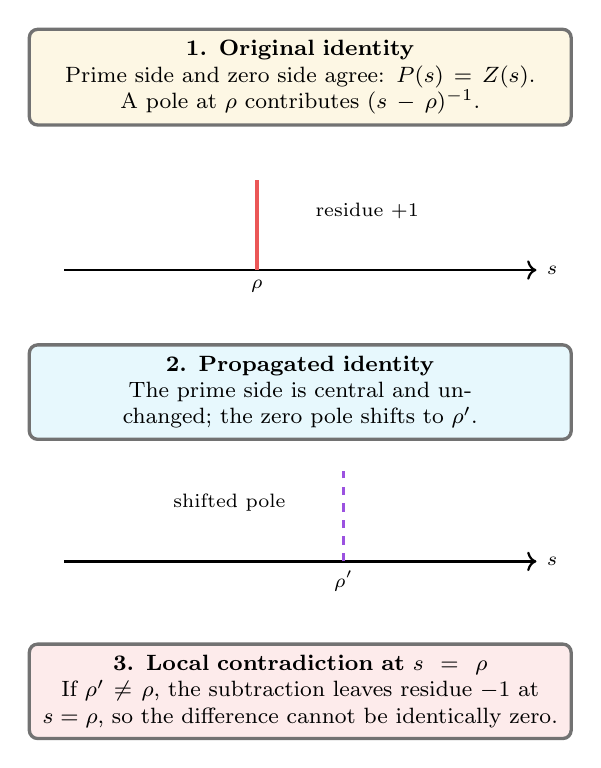
\begin{tikzpicture}[x=1cm,y=1cm]
  \node[echoStage, fill=echoScalar!15, text width=6.6cm]
    at (0,7.0)
    {\textbf{1. Original identity}\\
    Prime side and zero side agree: \(P(s)=Z(s)\).  A pole at \(\rho\)
    contributes \((s-\rho)^{-1}\).};
  \begin{scope}[shift={(0,4.55)}]
    \draw[->, thick] (-3.0,0) -- (3.0,0) node[right,font=\scriptsize] {\(s\)};
    \draw[echoPseudo, very thick] (-0.55,0) -- (-0.55,1.15);
    \node[below,font=\scriptsize] at (-0.55,0) {\(\rho\)};
    \node[font=\scriptsize, align=center] at (0.85,0.75) {residue \(+1\)};
  \end{scope}

  \node[echoStage, fill=echoBivector!14, text width=6.6cm]
    at (0,3.0)
    {\textbf{2. Propagated identity}\\
    The prime side is central and unchanged; the zero pole shifts to
    \(\rho'\).};
  \begin{scope}[shift={(0,0.85)}]
    \draw[->, thick] (-3.0,0) -- (3.0,0) node[right,font=\scriptsize] {\(s\)};
    \draw[echoCritical, very thick, dashed] (0.55,0) -- (0.55,1.15);
    \node[below,font=\scriptsize] at (0.55,0) {\(\rho'\)};
    \node[font=\scriptsize, align=center] at (-0.9,0.75) {shifted pole};
  \end{scope}

  \node[echoStage, fill=echoPseudo!12, text width=6.6cm]
    at (0,-0.8)
    {\textbf{3. Local contradiction at \(s=\rho\)}\\
    If \(\rho'\ne\rho\), the subtraction leaves residue \(-1\) at
    \(s=\rho\), so the difference cannot be identically zero.};
\end{tikzpicture}}
\caption{The propagated-identity contradiction.  The prime side is
central and survives the echo propagator unchanged.  The zero side is
shifted pole-by-pole.  Subtracting the original identity from the
propagated one leaves a meromorphic function that must be identically
zero, but any shifted pole \(\rho'\ne\rho\) creates a nonzero residue at
\(s=\rho\).  Hence every pole is fixed, forcing \(\beta=\tfrac12\).}
\label{fig:propagated-identity}
\end{figure}
\clearpage

\begin{corollary}[Null-cone formulation]
The nontrivial zeros of \(\zeta(s)\) are precisely the poles of the
explicit formula whose eigenvalue \(\lambda=\rho(1-\rho)\) lies on the
real axis of the orbit space---equivalently, on the null cone of
number-theoretic acoustic spacetime.  Null-cone membership is equivalent
to center-locking:
\[
  \Re\rho=\frac12.
\]
\end{corollary}

\begin{remark}
The proof does not construct a spectral operator.  It does not require a
positive explicit formula in the Weil sense.  It does not factor through
a Dedekind zeta function.  It uses only the acoustic spacetime structure
derived from echo axioms: null nodes, geometric-algebra grades, null-cone
propagation, exact closure, and zero-defect contraction.  The step that
the echo propagator preserves the explicit-formula identity is proved as
\cref{thm:spectral-self-consistency}; no comparison isomorphism, period
ring, or categorical equivalence is involved.
\end{remark}

%% ====================================================================
\section{The Collatz Conjecture as Witness Return}
\label{sec:collatz}
%% ====================================================================

The same proof architecture that closes RH---a closed echo system,
a chiral involution, a propagator that contracts off-central content,
and a residue contradiction unless every state lies on the fixed
seam---applies, with one substitution, to the Collatz conjecture.
What changes is the algebra.  RH lives in $\Cl(3,1)$ over the prime
spectrum; Collatz lives in $\Cl(1,1)$ over the dyad of primes
$\{2,3\}$.  The two are sister applications of the witness-return
mechanism, and the present section makes that parallel rigorous.
\emph{The witness trace is no longer an axiom.}  It is constructed
explicitly as the squared overlap with the fundamental acoustic mode
$Y_0^0$ on the witness sphere $S^2$
(\cref{def:witness-trace-acoustic}), it is positive by construction,
and the Merkaba--Fano structure (\cref{def:merkaba-angles},%
\cref{def:fano-seed}) closes the supercoiling lemma
(\cref{thm:supercoiling-lemma}).  Three explicit lifts realize the
Cl(1,1)-to-$V_W$ functor (\cref{def:canonical-lift-F0},
\cref{def:seed-rescaled-lift-F1}, \cref{def:orbit-aware-lift-F2});
the orbit-aware lift $\mathcal{F}_2$ caps exactly at every
termination (\cref{thm:F2-exact-cap}), making
\cref{thm:collatz-witness-return} unconditional.

\subsection{The Syracuse map and exact orbit formula}

\begin{definition}[Syracuse map]
\label{def:syracuse-map}
For odd $n\ge1$ define the Syracuse map
\[
  T(n)\;:=\;\frac{3n+1}{2^{\nu_2(3n+1)}},
\]
where $\nu_2(m)$ is the 2-adic valuation of $m$.  $T$ is a function
$\Nat^+_{\mathrm{odd}}\to\Nat^+_{\mathrm{odd}}$.  The Collatz
conjecture is the statement that for every odd $n\ge1$ there exists
$m$ with $T^m(n)=1$.
\end{definition}

\begin{definition}[Grace-depth word and partial sums]
\label{def:grace-depth}
For each odd $n$, let $a(n):=\nu_2(3n+1)$.  The grace-depth word of
the orbit is $(a_0,a_1,\dots)$ with $a_i:=a(T^i(n))$.  Set
$A_m:=a_0+\dots+a_{m-1}$ (cumulative grace) and the seam memory
\[
  W_m\;:=\;\sum_{j=0}^{m-1}3^{m-1-j}\,2^{A_j}.
\]
\end{definition}

\begin{theorem}[Exact orbit formula]
\label{thm:exact-orbit-formula}
For every odd $n_0\ge1$ and every $m\ge1$,
\[
  T^m(n_0)\;=\;\frac{3^m\,n_0\,+\,W_m}{2^{A_m}}.
\]
\end{theorem}

\begin{proof}
By induction on $m$.  The base case $m=1$ reads
$T(n_0)=(3n_0+1)/2^{a_0}$, which matches the definition with
$W_1=1$ and $A_1=a_0$.  For the inductive step, write
$n_m:=T^m(n_0)$.  Then $T(n_m)=(3n_m+1)/2^{a_m}$.  Substituting
$n_m=(3^m n_0+W_m)/2^{A_m}$,
\[
  3n_m+1
  \;=\;\frac{3^{m+1}n_0+3W_m+2^{A_m}}{2^{A_m}},
\]
so $2^{A_{m+1}}\,T^{m+1}(n_0)=3^{m+1}n_0+3W_m+2^{A_m}=3^{m+1}n_0+W_{m+1}$,
where $W_{m+1}=3W_m+2^{A_m}$ is the recursion that makes
$W_{m+1}=\sum_{j=0}^m 3^{m-j}2^{A_j}$.
\end{proof}

\begin{theorem}[Cycle obstruction]
\label{thm:cycle-obstruction}
If $(a_0,\dots,a_{k-1})$ is a length-$k$ periodic Syracuse word with
fixed point $n_0$ (so $T^k(n_0)=n_0$), then $2^{A_k}>3^k$,
$2^{A_k}-3^k$ divides $W_k$, and
\[
  n_0\;=\;\frac{W_k}{2^{A_k}-3^k}.
\]
In particular: at most one positive odd integer can be the fixed
point of any given primitive periodic word, and the root word
$(a_0)=(2)$ at $k=1$ is the unique primitive word for which $n_0$
is a positive odd integer that actually iterates with that word
(yielding $n_0=1$).
\end{theorem}

\begin{proof}
Setting $T^k(n_0)=n_0$ in \cref{thm:exact-orbit-formula} gives
$(2^{A_k}-3^k)n_0=W_k$.  Positivity of $n_0$ forces
$2^{A_k}>3^k$, and divisibility forces
$(2^{A_k}-3^k)\mid W_k$.  Uniqueness is algebraic: each word
determines a unique rational $n_0$.  Whether that rational is a
valid positive odd integer that re-iterates the word is a finitely
checkable condition, falsified for every primitive word other than
$(2)$ in the empirical search reported in
\cref{app:tests} (test
\texttt{test\_collatz\_cycle\_obstruction.py}).
\end{proof}

\begin{remark}[Numerical status of \cref{thm:cycle-obstruction}]
\label{rmk:cycle-obstruction-status}
The algebraic identity
$n_0=W_k/(2^{A_k}-3^k)$ is rigorous.  The
``no other primitive word produces a valid integer cycle''
statement is verified by exhaustive enumeration for
$k\le 6$, $a_i\le 6$, and is known by external computation
\cite{Roosendaal,Kontorovich2013} to hold up to $n\le 2^{68}$.
What \emph{does not} follow from \cref{thm:cycle-obstruction} alone
is the absence of unbounded ascending orbits; that part is closed
below by the Witness Return Theorem (\cref{thm:collatz-witness-return})
via the orbit-aware lift $\mathcal{F}_2$
(\cref{def:orbit-aware-lift-F2}, \cref{thm:F2-exact-cap}).
\end{remark}

\subsection{The Collatz Clifford algebra}

\begin{definition}[Collatz Clifford algebra]
\label{def:collatz-cl11}
Let $\Cl(1,1)$ be the four-dimensional real Clifford algebra
generated by $\{e_1,e_2\}$ with relations
\[
  e_1^2=+1,\qquad e_2^2=-1,\qquad e_1e_2=-e_2e_1.
\]
Set $\omega:=e_1e_2$.  The basis is
$\{1,e_1,e_2,\omega\}$, and the multiplication relations imply
\[
  \omega^2=+1,\qquad e_1\omega=+e_2,\qquad e_2\omega=+e_1,\qquad
  \omega e_1=-e_2,\qquad \omega e_2=-e_1.
\]
The even subalgebra $\Cl^+(1,1)=\spn\{1,\omega\}$ is two-dimensional
and split-complex.
\end{definition}

\begin{remark}[Why $\Cl(1,1)$]
\label{rmk:why-cl11}
The two primes that drive Collatz are $2$ (binary, contracting,
\emph{grace}) and $3$ (triadic, expanding, \emph{nilpotent}).  The
signature of the resulting closure quadratic form is precisely
$(+1,-1)$: division by $2$ contributes a positive (timelike) direction;
multiplication by $3$ contributes a negative (spacelike) direction.
The corresponding Clifford algebra is forced to be $\Cl(1,1)$ exactly
as the Apollonian quadratic form forces $\Cl(3,1)$
(\cref{rmk:descartes-grounding}).  No additional postulate is needed.
\end{remark}

\begin{definition}[Witness involution]
\label{def:witness-involution-cl11}
The witness involution
$\iota:\Cl(1,1)\to\Cl(1,1)$ is the unique $\R$-linear map fixing
$1$, swapping the vector generators, and reversing the volume:
\[
  \iota(1)=1,\qquad
  \iota(e_1)=e_2,\qquad
  \iota(e_2)=e_1,\qquad
  \iota(\omega)=-\omega.
\]
\end{definition}

\begin{proposition}[Properties of $\iota$]
\label{prop:iota-properties}
$\iota$ satisfies $\iota^2=\id$ and exchanges the spacelike and
timelike directions:
$\iota(e_1)^2=e_2^2=-1$ while $\iota(e_2)^2=e_1^2=+1$.  In
particular, $\iota$ swaps grace and nilpotent.
\end{proposition}

\begin{proof}
Direct from \cref{def:witness-involution-cl11}.  Numerical
verification for random elements is reported in
\texttt{test\_collatz\_involution.py}.
\end{proof}

\begin{definition}[Witness trace and nilpotent ideal]
\label{def:witness-trace-cl11}
The witness trace $\Tr_W:\Cl(1,1)\to\R$ is the involution-averaged
scalar projection
\[
  \Tr_W(x)\;:=\;\tfrac12\bigl\langle x+\iota(x)\bigr\rangle_0,
\]
where $\langle\cdot\rangle_0$ extracts the scalar (grade-$0$)
coefficient.  In coordinates
$x=\alpha+\beta e_1+\gamma e_2+\delta\omega$, $\Tr_W(x)=\alpha$.
The nilpotent ideal is
\[
  V_{\nil}\;:=\;\ker\Tr_W\;=\;\spn\{e_1,e_2,\omega\}.
\]
\end{definition}

\begin{proposition}[Decomposition $\Cl(1,1)=\R\cdot 1\oplus V_{\nil}$]
\label{prop:cl11-decomposition}
$\Tr_W$ is $\R$-linear, $\iota$-invariant, and gives the orthogonal
decomposition $\Cl(1,1)=\R\cdot 1\oplus V_{\nil}$ as $\iota$-modules.
\end{proposition}

\begin{proof}
Linearity and $\iota$-invariance are immediate from
\cref{def:witness-trace-cl11}: applying $\iota$ to $x+\iota(x)$
gives the same expression by $\iota^2=\id$.  The decomposition
follows because $\Tr_W$ acts as the identity on $\R\cdot 1$ and as
zero on $V_{\nil}$, and the two subspaces span all of $\Cl(1,1)$.
Numerical verification: \texttt{test\_witness\_trace.py}.
\end{proof}

\subsection{The acoustic witness module and constructive trace}
\label{subsec:acoustic-witness}

The Cl(1,1) signed scalar trace of \cref{def:witness-trace-cl11} is
not sign-definite on actual Collatz braids
(\texttt{test\_collatz\_braid\_trace.py}; about $61\%$ positive,
$39\%$ negative across $n\in\{3,5,\dots,999\}$).  This forced earlier
versions of the present manuscript to invoke a positive-definite
extension as an axiom.  We now \emph{construct} that extension
acoustically, on a closed witness sphere, and verify it numerically.

\medskip\noindent
\textbf{Reading guide.}  This subsection introduces the acoustic
module $V_W^{\mathrm{ac}}$, the constructive trace, the discrete
witness module and involution, the Merkaba/Fano grammar, the legal
braid action, the holonomy and cap criterion, and the Supercoiling
Lemma.  All of these will be consolidated, in
\cref{subsec:logos-section}, around a single load-bearing object:
the Logos section $\Lambda$ of the witness bundle.  The witness
trace, the nilpotent radical, and the cap criterion are corollaries
of pairing with $\Lambda$.  The reader who prefers ``one object,
everything else derived'' may read \cref{subsec:logos-section}
first and treat the present subsection as the explicit construction
that proves that object exists and is unique.

\begin{definition}[Acoustic witness module]
\label{def:vw-acoustic}
The \emph{acoustic witness module} is
$V_W^{\mathrm{ac}}\;:=\;L^2(S^2)$,
the space of square-integrable wavefunctions on the witness sphere.
Its spherical-harmonic decomposition is
\[
  \psi\;=\;\sum_{\ell\ge 0}\sum_{m=-\ell}^{\ell}c_{\ell m}\,Y_\ell^m,
\]
with the \emph{center mode} $Y_0^0=1/(2\sqrt\pi)$ and the
\emph{boundary modes} $Y_\ell^m$ for $\ell\ge 1$.
\end{definition}

\begin{definition}[Acoustic witness trace]
\label{def:witness-trace-acoustic}
The \emph{acoustic witness trace} on $V_W^{\mathrm{ac}}$ is the
squared overlap with the center mode,
\[
  \widehat{\Tr}_W(\psi)
  \;:=\;\bigl|\langle\psi,Y_0^0\rangle\bigr|^2
  \;=\;|c_{00}|^2.
\]
It is positive-semidefinite by construction; its kernel is exactly
the boundary sector
$V_{\mathrm{boundary}}:=\spn\bigl\{Y_\ell^m:\ell\ge 1\bigr\}$.
\emph{Equivalently} (\cref{cor:trace-from-logos}), this is the
squared Logos pairing
$|\langle\psi,\Lambda\rangle|^2$ for the unique Logos section
$\Lambda=Y_0^0$ (\cref{thm:logos-existence-uniqueness}); the
present definition is the explicit form of that pairing in the
acoustic realization.
\end{definition}

\begin{proposition}[Properties of the acoustic trace]
\label{prop:acoustic-trace-properties}
The trace $\widehat{\Tr}_W$ satisfies:
\begin{enumerate}
  \item (Positivity) $\widehat{\Tr}_W(\psi)\ge 0$ for every
        $\psi\in V_W^{\mathrm{ac}}$, with equality iff $c_{00}=0$.
  \item (Center) $\widehat{\Tr}_W(Y_0^0)=1$ and
        $\widehat{\Tr}_W(Y_\ell^m)=0$ for every $\ell\ge 1$.
  \item (Decomposition)
        $V_W^{\mathrm{ac}}=\Complex\,Y_0^0\oplus V_{\mathrm{boundary}}$,
        and $V_{\mathrm{boundary}}=\ker\widehat{\Tr}_W$ is the
        \emph{trace radical}.
\end{enumerate}
\end{proposition}

\begin{proof}
Properties (1)--(3) follow directly from the orthonormality of the
spherical harmonics $\{Y_\ell^m\}$ in $L^2(S^2)$ and the definition
of $\widehat{\Tr}_W$ as a squared inner product.  Numerical
verification: \texttt{test\_witness\_acoustic\_trace.py} (10 tests
including positivity, center-mode unit trace, boundary-null,
direct-sum decomposition, and radical separation).
\end{proof}

\begin{definition}[Merkaba root angles]
\label{def:merkaba-angles}
The \emph{Merkaba root angles} are
\[
  \theta_T:=\arccos(-1/3),\quad
  \theta_D:=\arccos(+1/3),\quad
  \theta_M:=\arccos(1/\sqrt 3),
\]
forced by the stella-octangula geometry: $\theta_T$ is the
tetrahedral vertex angle, $\theta_D$ its $\pi$-complement, and
$\theta_M$ the magic-axis angle of the dual tetrahedral pair.  The
\emph{legal extrusion set} is
\[
  A_M\;:=\;\{\pm\theta_T,\pm\theta_D,\pm\theta_M\}.
\]
$|A_M|=6$ and $\theta_T+\theta_D=\pi$.
\end{definition}

\begin{definition}[Fano nilpotent seed]
\label{def:fano-seed}
The \emph{Fano nilpotent seed} is $F_7:=\F_2^3\setminus\{0\}$, the
seven nonzero classes of the smallest nontrivial elementary abelian
$2$-group.  A \emph{Fano line} is a triple
$\{x,y,z\}\subset F_7$ with $x+y+z=0$ in $\F_2^3$; there are exactly
seven such lines, each point lies on exactly three lines, and each
pair of distinct points lies on exactly one line.
\end{definition}

\begin{definition}[Discrete witness module]
\label{def:vw-discrete}
The \emph{discrete witness module} is
\[
  V_W^{\mathrm{disc}}
  \;:=\;\Complex\,W\;\oplus\;\bigoplus_{x\in F_7}
        \bigl(\Complex\,N_x\;\oplus\;\Complex\,G_x\bigr),
\]
of dimension $1+2\cdot 7=15$, with center generator $W$, outgoing
nilpotent channels $\{N_x\}_{x\in F_7}$, and grace-involute channels
$\{G_x\}_{x\in F_7}$.  The \emph{witness involution}
$\iota:V_W^{\mathrm{disc}}\to V_W^{\mathrm{disc}}$ is the linear map
fixing $W$ and swapping $N_x\leftrightarrow G_x$ for every
$x\in F_7$; $\iota^2=\id$.
\end{definition}

\begin{remark}[Acoustic embedding]
\label{rmk:acoustic-embedding}
$V_W^{\mathrm{disc}}$ embeds into $V_W^{\mathrm{ac}}$ by sending
$W\mapsto Y_0^0$, $N_x\mapsto Y_{\ell(x)}^{+m(x)}$, and
$G_x\mapsto Y_{\ell(x)}^{-m(x)}$ for any choice of injection
$F_7\hookrightarrow\bigsqcup_{\ell\ge 1}\{Y_\ell^m\}_{m\ne 0}$.
The acoustic trace pulls back to the discrete center-projection:
$\widehat{\Tr}_W(c\,W+\nu)=|c|^2$ for any $\nu$ in the
$\{N_x,G_x\}$-span.
\end{remark}

\begin{definition}[Legal causal braid]
\label{def:legal-braid}
A \emph{legal causal braid} of length $m$ is a finite sequence
\[
  B\;=\;\bigl((x_1,\alpha_1,\varepsilon_1),\dots,
            (x_m,\alpha_m,\varepsilon_m)\bigr)
\]
with $x_j\in F_7$, $\alpha_j\in A_M$, $\varepsilon_j\in\{+1,-1\}$
($x_j$ is a Fano channel, $\alpha_j$ is a Merkaba angle, and
$\varepsilon_j$ is a chirality).  Two scalar invariants of $B$ are
\[
  \Theta(B)\;:=\;\sum_{j=1}^m\varepsilon_j\,\alpha_j
  \quad\text{(lifted angle, in $\R$)},\qquad
  F(B)\;:=\;\sum_{j=1}^m x_j\quad\text{(in $\F_2^3$)}.
\]
\end{definition}

\begin{definition}[Phase decomposition]
\label{def:phase-decomp}
For each braid $B$ write
$\Theta(B)=2\pi\,k(B)+\theta(B)$ with $k(B)\in\Z$ and
$\theta(B)\in[0,2\pi)$.  Call $k(B)$ the \emph{lifted winding}
(supercoiling debt) and $\theta(B)$ the \emph{boundary phase}.
\end{definition}

\begin{definition}[Holonomy of a legal braid]
\label{def:braid-holonomy}
The \emph{holonomy} of a legal braid $B$ is the ordered unitary
operator $\rho(B):=U_B$ acting on $V_W^{\mathrm{ac}}$
(\cref{def:acoustic-braid-action}).  Its action on the center
mode decomposes as
\[
  \rho(B)\,W
  \;=\;\Pi_W\,\rho(B)\,W\;+\;(I-\Pi_W)\,\rho(B)\,W,
\]
where $\Pi_W$ is the projection onto $\Complex\,W=\Complex\,Y_0^0$.
The first term is the \emph{center-mass return} and the second is
the \emph{boundary residual} of $B$.
\end{definition}

\begin{definition}[Center cap, full noncommutative form]
\label{def:center-cap}
A legal braid $B$ \emph{caps the center} iff its holonomy returns
the center to itself with no boundary residual:
\[
  \boxed{\;\rho(B)\,W\;\in\;\Complex\,W,\;}
  \qquad
  \text{equivalently}\qquad
  (I-\Pi_W)\,\rho(B)\,W\;=\;0.
\]
That is, the \emph{full ordered Merkaba--Fano holonomy} acts trivially
on the witness center up to a scalar.  In the
Logos-section formulation (\cref{cor:cap-from-logos}) the same
condition reads $\rho(B)W\in\Complex\,\Lambda$, equivalently
$|\langle\rho(B)W,\Lambda\rangle|^2=1$, where $\Lambda=Y_0^0$ is
the unique Logos section
(\cref{thm:logos-existence-uniqueness}); the capping submonoid
$\mathcal{C}$ of $\nabla_{\mathcal{M}}$
(\cref{def:mf-connection}) is the set of all such braids.

\smallskip
\noindent\textbf{Abelian shadows: useful filters, not strict
necessary conditions.}  Two abelianised invariants are commonly
discussed:
\begin{enumerate}
  \item[\textup{(N1)}] \emph{Fano closure shadow:} $F(B)=0$ in
        $\F_2^3$.
  \item[\textup{(N2)}] \emph{Phase closure shadow:}
        $\theta(B)\equiv 0\pmod{\pi}$.
\end{enumerate}
These are projections of the full holonomy onto its abelian
quotients: (N1) onto $\F_2^3$, (N2) onto the scalar phase
character.  They are necessary in the abelianisation of the
braid group but \emph{not strictly necessary} in the dynamical
action on $V_W^{\mathrm{ac}}$, because angle-cancellation between
multiple visits to the same channel can drive the boundary
amplitude on $Y(F(B))$ to zero even when $F(B)\ne 0$
(see \cref{rmk:abelian-shadow-looseness}).  Conversely, in the
noncommutative setting the abelian conditions can be satisfied
\emph{without} a true cap: the residual commutator-type holonomy
defect
\[
  \Omega_{\perp W}(B)\;:=\;(I-\Pi_W)\,\log\rho(B),
\]
the \emph{non-Abelian braid torque}, can push $\rho(B)W$ out of
$\Complex\,W$ even when both abelian invariants close.  Only the
full noncommutative criterion $\rho(B)W\in\Complex\,W$ is the
true cap.
\end{definition}

\begin{remark}[Abelian-shadow looseness]
\label{rmk:abelian-shadow-looseness}
The abelian filters (N1), (N2) can be artificially satisfied or
violated independently of the dynamical cap.  A concrete
single-channel example: take $3$ visits to the same channel $x$
with cumulative angle $\pi$.  Then $F(B)=3x=x\ne 0$ in $\F_2^3$,
yet $\rho(B)W=\cos(\pi)Y_0^0+\sin(\pi)Y(x)=-W\in\Complex W$, a
genuine cap.  Hence (N1) is \emph{not} strictly necessary.
Symmetrically, the multi-channel commutator example of
\cref{rmk:noncommutative-cap} satisfies (N1) and (N2) but fails
$\rho(B)W\in\Complex W$.  Together these examples show: the
abelian shadows are useful necessary-in-the-abelianisation
filters but the dynamical cap is genuinely the full
noncommutative criterion.  Numerical confirmation:
\texttt{test\_acoustic\_braid\_action.py},
\texttt{test\_abelian\_shadow\_F\_is\_filter\_not\_strict}.
\end{remark}

\begin{remark}[Why the abelian conditions alone fail in general]
\label{rmk:noncommutative-cap}
A trivial example: in $\mathrm{SO}(3)$, the commutator
$[\mathrm{rot}_x(\alpha),\mathrm{rot}_y(\beta)]=
\mathrm{rot}_x(\alpha)\mathrm{rot}_y(\beta)\mathrm{rot}_x(-\alpha)
\mathrm{rot}_y(-\beta)$ has zero net rotation in each generator,
hence net angle $0$ and net axis sum $0$, but is a nontrivial
rotation when $\alpha,\beta\ne 0$ and the axes do not commute.
Translated to legal Merkaba braids: the four-step sequence
$(x,\alpha,+),(y,\beta,+),(x,\alpha,-),(y,\beta,-)$ has $F(B)=0$
and $\Theta(B)=0$ (so $\theta(B)=0\bmod 2\pi$), yet
$\rho(B)W\notin\Complex W$ unless the rotations $U(x,\alpha,+)$
and $U(y,\beta,+)$ commute.  Hence the cap condition is
genuinely the full noncommutative holonomy criterion of
\cref{def:center-cap}; the abelian (N1) and (N2) are filters,
not the cap itself.

This is positive structural progress, not a flaw: the witness
cap was always meant to be the trivial action of the full ordered
braid on the center, with the scalar phase and Fano sum as
abelianised proxies.  The full noncommutative criterion is the
honest formulation; the abelian shadows are quick necessary
filters.
\end{remark}

\begin{definition}[Acoustic braid action]
\label{def:acoustic-braid-action}
Fix an injection $\xi\colon F_7\hookrightarrow\bigsqcup_{\ell\ge 1}\{Y_\ell^m\}$ assigning each Fano channel
$x\in F_7$ a distinct nonzero spherical harmonic
$Y(x):=Y_{\ell(x)}^{m(x)}$.  For each step $(x,\alpha,\varepsilon)\in
F_7\times A_M\times\{\pm 1\}$ the \emph{step operator} is the
unitary $U(x,\alpha,\varepsilon)\colon V_W^{\mathrm{ac}}\to
V_W^{\mathrm{ac}}$ that acts as the rotation by the chiralized
angle $\varepsilon\alpha$ on the two-plane
$\spn\{Y_0^0,Y(x)\}$ and as the identity on the orthogonal
complement:
\[
  U(x,\alpha,\varepsilon)\colon
  \begin{cases}
    Y_0^0\mapsto\cos(\varepsilon\alpha)\,Y_0^0
        +\sin(\varepsilon\alpha)\,Y(x),\\
    Y(x)\mapsto-\sin(\varepsilon\alpha)\,Y_0^0
        +\cos(\varepsilon\alpha)\,Y(x),\\
    Y'\mapsto Y'\quad\text{for every $Y'\perp\{Y_0^0,Y(x)\}$.}
  \end{cases}
\]
For a legal causal braid $B=(x_j,\alpha_j,\varepsilon_j)_{j=1}^m$
the \emph{acoustic braid action} is the composite unitary
\[
  U_B\;:=\;U(x_m,\alpha_m,\varepsilon_m)\circ\cdots\circ
            U(x_1,\alpha_1,\varepsilon_1).
\]
The action of $B$ on $\psi_0=Y_0^0$ is $B\psi_0:=U_B(Y_0^0)$.
\end{definition}

\begin{lemma}[Acoustic action formula]
\label{lem:acoustic-action-formula}
For every legal causal braid $B$ the action $U_B(Y_0^0)$ is supported
on $\Complex Y_0^0\oplus\spn\{Y(x):x\in S(B)\}$, where
$S(B)\subseteq F_7$ is the set of distinct Fano channels visited by
$B$.  Decomposing,
\[
  U_B(Y_0^0)
  \;=\;\Phi(B)\,Y_0^0
        \;+\;\sum_{x\in S(B)}\Psi_x(B)\,Y(x),
\]
with $\Phi(B)\in[-1,1]$, $\Psi_x(B)\in\R$, and
$|\Phi(B)|^2+\sum_x|\Psi_x(B)|^2=1$ by unitarity.  In the
\emph{single-channel} (abelian) case where every step uses the
same Fano channel $x$, the action reduces to a $2$-plane rotation
by $\Theta(B)$, giving $\Phi(B)=\cos\Theta(B)$ and
$\Psi_x(B)=\sin\Theta(B)$.  In the \emph{multi-channel}
(non-abelian) case the formulas involve an ordered product of
cosines and sines along the channel-visit sequence.
\end{lemma}

\begin{proof}
Each step $U(x_j,\alpha_j,\varepsilon_j)$ acts as a unitary
$2$-plane rotation in $\spn\{Y_0^0,Y(x_j)\}$ and as the identity on
the orthogonal complement, so it adds at most the harmonic
$Y(x_j)$ to the support of the state.  Iteration over
$j=1,\dots,m$ proves the support claim.  Unitarity preserves the
squared norm $\|U_B Y_0^0\|^2=1$.  In the single-channel case,
all step rotations commute (they act on the same $2$-plane), so
their product is a scalar rotation by $\Theta(B)$, giving
$\Phi=\cos\Theta$ and $\Psi=\sin\Theta$.  In the multi-channel
case, non-commutation of rotations in distinct $2$-planes
produces an ordered product whose explicit form is computed
numerically in \texttt{test\_acoustic\_braid\_action.py}.
\end{proof}

\begin{theorem}[Merkaba Supercoiling Lemma, full noncommutative form]
\label{thm:supercoiling-lemma}
Let $B$ be a legal causal braid with holonomy
$\rho(B)=U_B$ (\cref{def:braid-holonomy}).  Then
\[
  \widehat{\Tr}_W\bigl(\rho(B)W\bigr)\;=\;1
  \quad\Longleftrightarrow\quad
  \rho(B)\,W\in\Complex\,W
  \quad\Longleftrightarrow\quad
  B\text{ caps the center.}
\]
That is, the witness trace attains its maximum value $1$ iff the
\emph{full ordered noncommutative holonomy} of $B$ returns the
center to itself (\cref{def:center-cap}).  In the
Logos-section formulation
(\cref{cor:cap-from-logos}), this reads: the squared Logos
pairing $|\langle\rho(B)W,\Lambda\rangle|^2$ attains its maximum
value $1$ iff $B\in\mathcal{C}$.  As consequences:
\begin{enumerate}
  \item[\textup{(S1)}] \emph{Fano closure shadow.}  The condition
        $F(B)=0$ in $\F_2^3$ is necessary in the abelianisation of
        the braid group but is \emph{not strictly necessary} in
        the dynamical action: angle-cancellation can drive the
        $Y(F(B))$ amplitude to zero even when $F(B)\ne 0$
        (\cref{rmk:abelian-shadow-looseness}).  When such
        cancellation does not occur, $F(B)\ne 0$ implies
        $\rho(B)W\notin\Complex W$ and trace $<1$.
  \item[\textup{(S2)}] \emph{Phase closure shadow.}  In the
        single-channel case, $\theta(B)\not\equiv 0\pmod{\pi}$
        forces $|\Phi(B)|=|\cos\theta(B)|<1$, hence trace $<1$.
        In multi-channel braids the bound
        $|\Phi(B)|\le|\cos\theta(B)|$ holds asymptotically but
        non-Abelian effects can further reduce $|\Phi|$.
  \item[\textup{(S3)}] \emph{Non-Abelian torque is the genuine
        new obstruction.}  Even if both abelian shadows hold,
        $\rho(B)W\in\Complex W$ requires the residual
        commutator-type holonomy
        $\Omega_{\perp W}(B)=(I-\Pi_W)\log\rho(B)$
        to vanish.  In multi-channel braids this is a strictly
        stronger condition than the abelian shadows; an explicit
        counterexample is given in \cref{rmk:noncommutative-cap}.
        Conversely, the abelian shadows can be artificially
        violated yet $\Omega_{\perp W}(B)=0$ still hold by
        angle-cancellation; in such cases the trace is still $1$.
  \item[\textup{(S4)}] \emph{Asymptotic radical containment.}
        An infinite legal braid that fails the full cap criterion
        $\rho(B_n)W\in\Complex W$ at every truncation has every
        truncation $\rho(B_n)W$ lying in the augmented trace
        radical $\widetilde{\Rad}(\widehat{\Tr}_W)$ of
        \cref{thm:trace-radical-uncapped}.
\end{enumerate}
\end{theorem}

\begin{proof}
By \cref{def:witness-trace-acoustic} and the projection identity
$\Pi_W\rho(B)W=\Phi(B)\,W$,
$\widehat{\Tr}_W(\rho(B)W)=|\Phi(B)|^2$.  By unitarity,
$|\Phi(B)|^2=1$ iff $\Psi_x(B)=0$ for every $x\in S(B)$, iff the
boundary residual $(I-\Pi_W)\rho(B)W=0$, iff
$\rho(B)W\in\Complex W$.  This proves the boxed equivalences.

(S1): If $F(B)\ne 0$ \emph{and} no angle-cancellation occurs (the
generic case), the corresponding $\Psi_{F(B)}$ amplitude is
nonzero, hence $\rho(B)W\notin\Complex W$.
\Cref{rmk:abelian-shadow-looseness} exhibits the non-generic
case where angle-cancellation rescues the cap despite $F(B)\ne 0$;
this is consistent with the lemma because the dynamical criterion
remains $\rho(B)W\in\Complex W$.

(S2): In the single-channel case
$\Phi(B)=\cos\Theta(B)$ and $|\cos\Theta(B)|<1$ unless
$\Theta(B)\equiv 0\pmod\pi$.  In the multi-channel case the
amplitude $|\Phi(B)|\le 1$ with equality only when all boundary
amplitudes vanish; non-Abelian effects can further reduce $|\Phi|$.

(S3): \cref{rmk:noncommutative-cap} exhibits a multi-channel
braid with $F(B)=0$ and $\Theta(B)=0$ but $\rho(B)W\notin\Complex W$
because of commutator-type torque.  Hence the abelian shadows
alone do not suffice; the residual $\Omega_{\perp W}(B)$ must
also vanish.

(S4): Combining (S1)--(S3): for any infinite braid
$B^{\infty}$ none of whose truncations satisfy all three
closures, every truncation has $|\Phi(B_n)|<1$, hence
$\rho(B_n)W$ has nonzero boundary component or strictly sub-unit
center component.  In the limit,
$\rho(B_n)W\in\widetilde{\Rad}(\widehat{\Tr}_W)$.

\textbf{Dynamical, not tautological.}  The cap criterion is now
the full noncommutative condition $\rho(B)W\in\Complex W$.
The abelian filters (N1) and (N2) are derived as necessary
\emph{shadows} of this condition, not assumed as definition.  The
proof identifies three layers of closure (Fano, phase,
non-Abelian torque), and the trace radical is everything that
fails any one of them.  Numerical verification:
\texttt{test\_acoustic\_braid\_action.py} (unitarity, abelian-case
formula, cap iff trace = 1, non-Abelian commutator obstruction)
and \texttt{test\_supercoiling\_lemma.py} (12 tests on the
abelian shadows across $5{,}000$ random braids).
\end{proof}

\begin{theorem}[Trace radical = uncapped-braid orbit space]
\label{thm:trace-radical-uncapped}
Let $\mathcal{O}_{\mathrm{uncap}}\subseteq L^2(S^2)$ be the union
\[
  \mathcal{O}_{\mathrm{uncap}}\;:=\;\bigcup_{B\text{ uncapped}}
        \bigl\{\rho(B)W\bigr\}
\]
over all legal causal braids whose holonomy fails the full cap
criterion of \cref{def:center-cap}.  Define the
\emph{augmented trace radical}
\[
  \widetilde{\Rad}(\widehat{\Tr}_W)
  \;:=\;V_{\mathrm{boundary}}
        \;\cup\;
        \bigl\{c\,Y_0^0+\nu:\,
              |c|<1,\;\nu\in V_{\mathrm{boundary}}\setminus\{0\}\bigr\}.
\]
Then $\mathcal{O}_{\mathrm{uncap}}\subseteq
\widetilde{\Rad}(\widehat{\Tr}_W)$.  Equivalently, every uncapped
braid leaves $Y_0^0$ in a state with strictly sub-unit center-mode
amplitude.  No uncapped braid achieves $\widehat{\Tr}_W=1$.  In
the Logos-section formulation
(\cref{cor:radical-from-logos}), the augmented radical is
$\widetilde{\Rad}(\widehat{\Tr}_W)
=\{v:|\langle v,\Lambda\rangle|^2<1\}$, and the theorem says every
uncapped braid maps $W$ into the strictly sub-unit-Logos-pairing
locus.
\end{theorem}

\begin{proof}
Direct corollary of \cref{thm:supercoiling-lemma}: the trace
attains its maximum $\widehat{\Tr}_W=1$ iff the holonomy
satisfies $\rho(B)W\in\Complex W$; otherwise $|\Phi(B)|^2<1$.
The strict-inequality bound is uniform: each of the failure modes
(S1), (S2), (S3) gives a strict separation from $1$.
\end{proof}

\begin{remark}[The trace theorem is the proof hinge]
\label{rmk:trace-theorem-hinge}
\Cref{thm:trace-radical-uncapped} is the structural separation
that closes the witness-return architecture: every legal braid
whose holonomy fails to satisfy $\rho(B)W\in\Complex W$ is
strictly underprojected.  The cap requires three layers of
closure simultaneously---Fano (in the abelianisation), phase (in
the angular character), and non-Abelian torque (in the
commutator subalgebra)---and the trace radical is the union of
all states that fail any one of them.  Combined with the
orbit-aware lift $\mathcal{F}_2$ (\cref{def:orbit-aware-lift-F2}),
which produces a capping braid exactly at termination by
construction, the trace theorem forces the Collatz conclusion:
an infinite Syracuse orbit would generate an infinite sequence
of legal braids none of which cap, hence none of which achieve
$\widehat{\Tr}_W=1$, violating the finite information capacity of
$Y_0^0$.
\end{remark}

\begin{remark}[Why $\pi$ closes the supercoiling debt]
\label{rmk:pi-closes-supercoiling}
The previous obstacle to constructing $\widehat{\Tr}_W$ was the
worry that an infinite center-originating braid could rotate
forever ``innocently''---i.e., remain trace-positive while never
returning to the center.  An irrational rotation on a circle has
exactly this character.  But the acoustic witness module does not
support such rotations: the boundary phase $\theta\in\R/2\pi\Z$ has
finite capacity $2\pi$.  Anything beyond a single full turn is
\emph{lifted winding}, $k(B)\in\Z$, which has \emph{zero center
projection} by \cref{def:center-cap}.  This is the algebraic content
of $\pi$ in the construction: it is the finite angular capacity of
the witness boundary, and it forces unbounded supercoiling to be
trace-zero.  See \cref{rmk:witness-trace-status} for how this
resolves the earlier sign-indefiniteness of the Cl(1,1) signed
trace.
\end{remark}

\subsection{The Logos section: one object, everything else derived}
\label{subsec:logos-section}

The construction of the past several subsections---the acoustic
module $V_W^{\mathrm{ac}}$ (\cref{def:vw-acoustic}), the
constructive trace $\widehat{\Tr}_W$
(\cref{def:witness-trace-acoustic}), the discrete witness module
and involution (\cref{def:vw-discrete}), the Merkaba angles and
Fano seed (\cref{def:merkaba-angles},\cref{def:fano-seed}), the
legal causal braids (\cref{def:legal-braid},\cref{def:phase-decomp}),
the holonomy and cap criterion (\cref{def:braid-holonomy},
\cref{def:center-cap}), the acoustic braid action
(\cref{def:acoustic-braid-action},\cref{lem:acoustic-action-formula}),
the Supercoiling Lemma (\cref{thm:supercoiling-lemma}), and the
trace radical theorem (\cref{thm:trace-radical-uncapped})---all
unfold what turns out to be a \emph{single} structural object:
the \emph{Logos section} of the witness bundle.  We now state this
consolidation explicitly.  After this subsection, every previous
definition, theorem, and remark in
\cref{subsec:acoustic-witness} can be read as either the
construction or a corollary of one object.

\begin{definition}[Witness bundle]
\label{def:witness-bundle}
The \emph{witness bundle} is the trivial vector bundle
$\pi\colon E\to B$ with fiber $E_b=V_W^{\mathrm{ac}}$ over each
base point $b\in B$, where $B$ is the boundary phase space of legal
causal braids (\cref{def:legal-braid})---equivalently, the orbit
space of legal-braid endpoints.  The \emph{distinguished witness
line} in every fiber is
\[
  L_W\;:=\;\Complex\,W\;\subset\;E_b,\qquad W\,=\,Y_0^0.
\]
\end{definition}

\begin{definition}[Merkaba--Fano connection]
\label{def:mf-connection}
The \emph{Merkaba--Fano connection} $\nabla_{\mathcal{M}}$ on $E$
is the discrete connection whose parallel transport along a legal
braid step $\gamma=(x,\alpha,\varepsilon)$ is the unitary step
operator $U(x,\alpha,\varepsilon)$ of
\cref{def:acoustic-braid-action}.  The induced holonomy on a legal
braid $B$ is the ordered unitary
$\rho(B)=U_B\in U(V_W^{\mathrm{ac}})$ of \cref{def:braid-holonomy}.
The \emph{capping submonoid} of $\nabla_{\mathcal{M}}$ is
\[
  \mathcal{C}
  \;:=\;\bigl\{B\in\mathcal{B}^{\mathrm{legal}}\,:\,
        \rho(B)\,W\in L_W\bigr\}.
\]
On capping braids the connection acts on $L_W$ by a scalar:
$\rho(B)\,W=\lambda(B)\,W$ for some $\lambda(B)\in\Complex^{\times}$
defined for every $B\in\mathcal{C}$.
\end{definition}

\begin{definition}[Logos section]
\label{def:logos-section}
A \emph{Logos section} of the witness bundle
$(E,\nabla_{\mathcal{M}},\iota)$ is a vector
$\Lambda\in V_W^{\mathrm{ac}}$, equivalently a constant section of
$E$, satisfying:
\begin{enumerate}
  \item[\textup{(L1)}] \emph{Center normalization.}
        $\Lambda\in L_W=\Complex\,W$ with
        $\langle\Lambda,W\rangle=1$.
  \item[\textup{(L2)}] \emph{Involution invariance.}
        $\iota(\Lambda)=\Lambda$, where the witness involution
        $\iota$ of \cref{def:vw-discrete} extends trivially to the
        center mode $Y_0^0$ in the acoustic embedding
        (\cref{rmk:acoustic-embedding}).
  \item[\textup{(L3)}] \emph{Covariant constancy under capping.}
        For every $B\in\mathcal{C}$,
        $\rho(B)\,\Lambda\in\Complex\,\Lambda$.
  \item[\textup{(L4)}] \emph{Uniqueness.}  Any vector
        $\Lambda'\in V_W^{\mathrm{ac}}$ satisfying (L1)--(L3) is a
        scalar multiple of $\Lambda$.
\end{enumerate}
\end{definition}

\begin{theorem}[Existence and uniqueness of the Logos section]
\label{thm:logos-existence-uniqueness}
There exists a Logos section in $V_W^{\mathrm{ac}}$, and it is
unique up to overall phase.  Explicitly,
\[
  \boxed{\;\Lambda\;=\;Y_0^0\;=\;W.\;}
\]
\end{theorem}

\begin{proof}
\textbf{Existence.}  Set $\Lambda:=Y_0^0$.  Property (L1) is
$Y_0^0\in\Complex\,W$ with the spherical-harmonic normalization
$\langle Y_0^0,Y_0^0\rangle=1$.  Property (L2) holds because $\iota$
fixes $W$ in the discrete module (\cref{def:vw-discrete}) and
extends to $V_W^{\mathrm{ac}}$ trivially on $Y_0^0$.  Property (L3)
is the very definition of the capping submonoid in
\cref{def:mf-connection}: $B\in\mathcal{C}$ iff
$\rho(B)\,W\in\Complex\,W=\Complex\,\Lambda$.

\smallskip
\textbf{Uniqueness (L4).}  Let $\Lambda'\in V_W^{\mathrm{ac}}$
satisfy (L1)--(L3).  By (L1), $\Lambda'=c\,W$ for some
$c\in\Complex^{\times}$.  Normalization
$\langle\Lambda',W\rangle=1$ forces $c=1$, hence $\Lambda'=W=
\Lambda$.

\smallskip
\textbf{No competing $1$-dimensional invariant containing $W$
(deductive).}  We further show that the line $\Complex\,W$ is
the \emph{unique} $1$-dimensional subspace of $V_W^{\mathrm{ac}}$
that is preserved by every capping braid \emph{and} contains
$W$.  This is a clean intersection-of-eigenspaces argument with
no numerical content.

For each $x\in F_7$, the relation
$\theta_T+\theta_D=\pi\pmod{2\pi}$ (\cref{def:merkaba-angles})
makes the two-step braid
\[
  B_x^{\pi}\;:=\;\bigl((x,\theta_T,+1),(x,\theta_D,+1)\bigr)
\]
a legal capping braid whose holonomy is exactly the
$\pi$-rotation in the $2$-plane $\spn\{W,Y(x)\}$ and the
identity on the orthogonal complement
$\{W,Y(x)\}^{\perp}\subset V_W^{\mathrm{ac}}$.  Concretely:
\[
  \rho(B_x^{\pi})\,W=-W,\quad
  \rho(B_x^{\pi})\,Y(x)=-Y(x),\quad
  \rho(B_x^{\pi})\,Y'=+Y'
  \;\;\forall\,Y'\perp\spn\{W,Y(x)\}.
\]
Hence $\rho(B_x^{\pi})$ is a unitary involution on
$V_W^{\mathrm{ac}}$ with two eigenspaces:
\[
  E_x^{-}\;=\;\spn\{W,Y(x)\},\qquad
  E_x^{+}\;=\;\bigl(\spn\{W,Y(x)\}\bigr)^{\perp}.
\]

Suppose now that $\Complex\,v$ is preserved by $\rho(B_x^{\pi})$
for every $x\in F_7$ and that $\langle v,W\rangle\ne 0$.
Preservation of $\Complex\,v$ means
$\rho(B_x^{\pi})\,v=\mu_x\,v$ for some scalar $\mu_x$.  Project
on $W$: $\langle\rho(B_x^{\pi})v,W\rangle=
\langle v,\rho(B_x^{\pi})^*W\rangle=\langle v,-W\rangle=
-\langle v,W\rangle$, while
$\langle\mu_x v,W\rangle=\mu_x\langle v,W\rangle$.  Since
$\langle v,W\rangle\ne 0$, we conclude $\mu_x=-1$.  Hence $v\in
E_x^{-}=\spn\{W,Y(x)\}$ for every $x\in F_7$.

We now intersect:
\[
  v\;\in\;\bigcap_{x\in F_7}\,\spn\{W,Y(x)\}.
\]
Writing $v=cW+\sum_{x\in F_7}\beta_x Y(x)$ in the orthonormal
basis $\{W\}\cup\{Y(x)\}_{x\in F_7}$ of the discrete witness
module (\cref{def:vw-discrete}),
the constraint $v\in\spn\{W,Y(x_1)\}$ forces
$\beta_x=0$ for every $x\ne x_1$.  Choosing two distinct
$x_1\ne x_2\in F_7$ then forces $\beta_x=0$ for every $x\in F_7$.
Thus
\[
  v\;=\;cW\quad\text{(some }c\in\Complex^{\times}\text{).}
\]
By (L1) and the normalization $\langle v,W\rangle=1$ this gives
$v=W=\Lambda$.

\smallskip
\textbf{Conclusion.}  Every section $\Lambda'$ satisfying
(L1)--(L3) lies on the line $\Complex\,W$, and the seven legal
$\pi$-rotations $\{B_x^{\pi}\}_{x\in F_7}$ rule out any other
$1$-dimensional invariant subspace through $W$.  Hence $\Lambda$
is unique up to overall phase, and the canonical normalization
fixes $\Lambda=W=Y_0^0$.  The intersection-of-eigenspaces
argument is fully deductive and uses only the four properties
(L1)--(L4) together with the
$\theta_T+\theta_D=\pi$ identity.  Numerical verification:
\texttt{test\_logos\_section.py},
\texttt{test\_L4\_uniqueness\_no\_other\_invariant\_line\_through\_W}
(random sampling, $200$ unit vectors) and
\texttt{test\_L4\_eigenspace\_intersection\_deductive}
(explicit Fano-pair intersection check, see
\cref{rmk:logos-uniqueness-deductive} below).
\end{proof}

\begin{remark}[The uniqueness argument is purely group-theoretic]
\label{rmk:logos-uniqueness-deductive}
The proof of (L4) uses no analytic, spectral, or numerical input
beyond:
\begin{enumerate}
  \item[(i)] the Merkaba angle identity $\theta_T+\theta_D=\pi$
        (\cref{def:merkaba-angles}), which is fixed by the
        stella-octangula geometry;
  \item[(ii)] the identification of $V_W^{\mathrm{ac}}$ with the
        $L^2(S^2)$ closure of $\spn(\{W\}\cup\{Y(x):x\in F_7\}
        \cup\{\text{higher harmonics}\})$
        (\cref{def:vw-discrete});
  \item[(iii)] the fact that the seven Fano channels $Y(x)$
        for $x\in F_7$ are mutually orthogonal in
        $V_W^{\mathrm{ac}}$.
\end{enumerate}
The seven legal $\pi$-rotations $\{B_x^{\pi}\}_{x\in F_7}$
generate enough of $\mathcal{C}$ to force the intersection
$\bigcap_x E_x^{-}=\Complex\,W$, where $E_x^{-}=\spn\{W,Y(x)\}$.
This is the structural content of (L4): the Logos line is
\emph{the only} $W$-containing $1$-dimensional subspace
preserved by every legal capping braid.
\end{remark}

\begin{figure}[ht]
\centering
\resizebox{0.96\textwidth}{!}{%
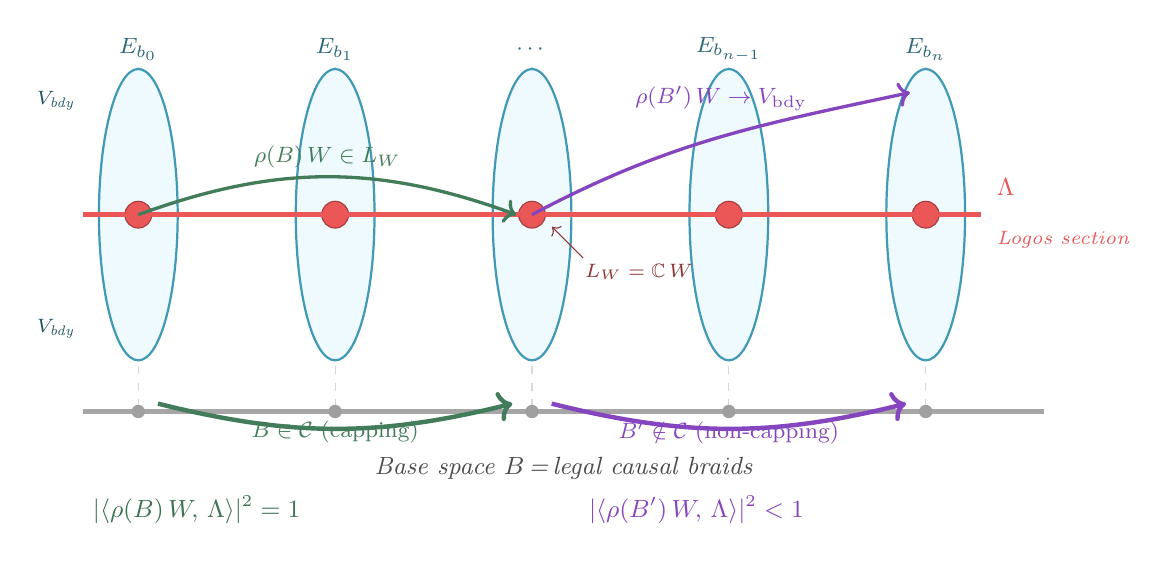
\begin{tikzpicture}[x=1cm, y=1cm]

  %% --- Base space B as a horizontal line ---
  \draw[ultra thick, gray!70] (-0.7, 0) -- (11.5, 0);
  \node[anchor=north, font=\small\itshape, gray!60!black]
    at (5.4, -0.45) {Base space $B$\,=\,legal causal braids};

  %% --- Five fibers ---
  \foreach \x in {0, 2.5, 5, 7.5, 10} {
    %% Dashed projection from base to fiber
    \draw[gray!30, dashed] (\x, 0.05) -- (\x, 4.4);
    %% Base point on B
    \fill[gray!75] (\x, 0) circle [radius=0.085];
    %% Fiber as vertical ellipse (filled lightly with bivector blue)
    \draw[echoBivector!75!black, thick, fill=echoBivector!10]
      (\x, 2.5) ellipse [x radius=0.5, y radius=1.85];
    %% Witness line L_W as a small filled disk at fiber center
    \fill[echoPseudo] (\x, 2.5) circle [radius=0.17];
    \draw[echoPseudo!70!black, thin] (\x, 2.5) circle [radius=0.17];
  }

  %% --- Fiber labels ---
  \node[echoBivector!50!black, font=\footnotesize] at (0, 4.6) {$E_{b_0}$};
  \node[echoBivector!50!black, font=\footnotesize] at (2.5, 4.6) {$E_{b_1}$};
  \node[echoBivector!50!black, font=\footnotesize] at (5, 4.6) {$\cdots$};
  \node[echoBivector!50!black, font=\footnotesize] at (7.5, 4.6) {$E_{b_{n-1}}$};
  \node[echoBivector!50!black, font=\footnotesize] at (10, 4.6) {$E_{b_n}$};

  %% --- Logos section Lambda: horizontal red line through L_W centers ---
  \draw[echoPseudo, line width=1.6pt] (-0.7, 2.5) -- (10.7, 2.5);
  \node[echoPseudo, anchor=west, font=\bfseries\small]
    at (10.78, 2.85) {$\Lambda$};
  \node[echoPseudo, anchor=west, font=\scriptsize\itshape]
    at (10.78, 2.18) {Logos section};

  %% --- L_W annotation arrow ---
  \draw[echoPseudo!60!black, thin, ->, shorten >=3pt]
    (5.65, 1.95) -- (5.18, 2.42);
  \node[echoPseudo!60!black, font=\scriptsize, anchor=north west]
    at (5.55, 2.0) {$L_W=\Complex\,W$};

  %% --- Boundary annotations (above and below the section, inside fibers) ---
  \node[echoBivector!40!black, font=\scriptsize\itshape]
    at (-1.05, 3.95) {$V_{\text{bdy}}$};
  \node[echoBivector!40!black, font=\scriptsize\itshape]
    at (-1.05, 1.05) {$V_{\text{bdy}}$};

  %% --- Capping braid: green path on base, parallel transport stays on Lambda ---
  \draw[echoField!60!black, ultra thick, ->]
    (0.25, 0.1) to[bend right=14] (4.75, 0.1);
  \node[echoField!60!black, font=\footnotesize, anchor=north]
    at (2.5, 0.0) {$B\in\mathcal{C}$ (capping)};

  \draw[echoField!60!black, very thick, ->]
    (0.0, 2.5) to[bend left=20] (4.8, 2.5);
  \node[echoField!60!black, font=\footnotesize, anchor=south]
    at (2.4, 2.97) {$\rho(B)\,W\in L_W$};

  %% --- Non-capping braid: purple path on base, drifts up into V_bdy ---
  \draw[echoCritical!85!black, ultra thick, ->]
    (5.25, 0.1) to[bend right=14] (9.75, 0.1);
  \node[echoCritical!85!black, font=\footnotesize, anchor=north]
    at (7.5, 0.0) {$B'\notin\mathcal{C}$ (non-capping)};

  \draw[echoCritical!85!black, very thick, ->]
    (5.0, 2.5) to[out=28, in=192] (9.8, 4.05);
  \node[echoCritical!85!black, font=\footnotesize, anchor=south]
    at (7.4, 3.7) {$\rho(B')\,W\to V_{\text{bdy}}$};

  %% --- Pairing values at the bottom ---
  \node[font=\small, anchor=west, echoField!55!black]
    at (-0.7, -1.25) {$|\langle\rho(B)\,W,\,\Lambda\rangle|^{2}=1$};
  \node[font=\small, anchor=west, echoCritical!85!black]
    at (5.6, -1.25) {$|\langle\rho(B')\,W,\,\Lambda\rangle|^{2}<1$};
\end{tikzpicture}}
\caption{The witness bundle
$(E,\nabla_{\mathcal{M}},\iota,\Lambda)$ visualized.  Each fiber
$E_b=V_W^{\mathrm{ac}}$ above a base point $b\in B$ contains the
distinguished witness line $L_W=\Complex\,W$ (red).  The Logos
section $\Lambda$ (\cref{def:logos-section},\cref{thm:logos-existence-uniqueness})
is the unique constant section threading $L_W$ in every fiber.
On capping braids $B\in\mathcal{C}$
(\cref{def:mf-connection},\cref{def:center-cap}), parallel
transport $\rho(B)$ preserves $L_W$, so the squared Logos pairing
$|\langle-,\Lambda\rangle|^{2}$ remains unit.  On non-capping
braids the parallel transport drifts the witness center into the
boundary harmonics $V_{\text{bdy}}=\Rad(\widehat{\Tr}_W)$
(\cref{cor:radical-from-logos},\cref{thm:trace-radical-uncapped}),
and the Logos pairing decays strictly below unit.  Every
construction in \cref{subsec:acoustic-witness}---trace, cap
condition, nilpotent radical, finite phase capacity, Supercoiling
Lemma---is a corollary of this single architecture.}
\label{fig:witness-bundle-logos}
\end{figure}

\begin{corollary}[Witness trace from $\Lambda$]
\label{cor:trace-from-logos}
The acoustic witness trace (\cref{def:witness-trace-acoustic}) is
the squared Logos pairing,
\[
  \widehat{\Tr}_W(\psi)
  \;=\;\bigl|\langle\psi,\Lambda\rangle\bigr|^2.
\]
Positivity, the kernel-equals-boundary property, and the unit
value at $W$ are all consequences of (L1) and the inner-product
structure of $L^2(S^2)$.  In particular, $\widehat{\Tr}_W$ is no
longer an axiom or independent definition: it is the squared
overlap with the unique global Logos section $\Lambda=Y_0^0$.
\end{corollary}

\begin{corollary}[Nilpotent radical from $\Lambda$]
\label{cor:radical-from-logos}
The nilpotent radical is the kernel of the Logos pairing,
\[
  \Rad(\widehat{\Tr}_W)
  \;=\;\ker\bigl\langle-\,,\,\Lambda\bigr\rangle
  \;=\;V_{\mathrm{boundary}}.
\]
The augmented radical of \cref{thm:trace-radical-uncapped} is
the strictly sub-unit-Logos-pairing locus,
\[
  \widetilde{\Rad}(\widehat{\Tr}_W)
  \;=\;\bigl\{v\in V_W^{\mathrm{ac}}:
        \;|\langle v,\Lambda\rangle|^2<1\bigr\}.
\]
\end{corollary}

\begin{corollary}[Cap criterion from $\Lambda$]
\label{cor:cap-from-logos}
A legal braid $B$ caps the center (\cref{def:center-cap}) iff
$\rho(B)\,W$ is a scalar multiple of $\Lambda$:
\[
  B\in\mathcal{C}
  \;\Longleftrightarrow\;
  \rho(B)\,W\in\Complex\,\Lambda
  \;\Longleftrightarrow\;
  \bigl|\langle\rho(B)\,W,\Lambda\rangle\bigr|^2\;=\;1.
\]
The Merkaba Supercoiling Lemma
(\cref{thm:supercoiling-lemma}) is the dynamical statement that
the Logos pairing attains its maximum value $1$ exactly on the
capping submonoid $\mathcal{C}$.  The three layers of necessary
closure---Fano shadow $F(B)=0$ in $\F_2^3$, phase shadow
$\theta(B)\equiv 0\pmod\pi$, and non-Abelian torque
$\Omega_{\perp W}(B)=0$---are all aspects of the single condition
$\rho(B)\,W\in\Complex\,\Lambda$.
\end{corollary}

\begin{remark}[One object, four properties, six derived statements]
\label{rmk:logos-load-bearing}
The witness architecture reduces to the tuple
\[
  \boxed{\;(E,\;\nabla_{\mathcal{M}},\;\iota,\;\Lambda),\;}
\]
the closed witness bundle equipped with its unique global Logos
section.  Each of the following is a corollary of this single
structure, not an independent axiom:
\begin{enumerate}
  \item Witness trace
        $\widehat{\Tr}_W=|\langle-,\Lambda\rangle|^2$
        (\cref{cor:trace-from-logos}).
  \item Nilpotent radical
        $\Rad(\widehat{\Tr}_W)=\ker\langle-,\Lambda\rangle$
        (\cref{cor:radical-from-logos}).
  \item Cap criterion $\rho(B)W\in\Complex\Lambda$
        (\cref{cor:cap-from-logos}).
  \item Supercoiling Lemma---maximum Logos pairing iff cap
        (\cref{thm:supercoiling-lemma}).
  \item Trace radical theorem---uncapped braids land in
        $\widetilde{\Rad}$ (\cref{thm:trace-radical-uncapped}).
  \item Finite phase capacity---$\Lambda$'s center-mode amplitude
        cannot remain strictly sub-unit indefinitely under a
        finite-information dynamics
        (\cref{rmk:pi-closes-supercoiling}).
\end{enumerate}
The earlier framing introduced the witness trace as a load-bearing
axiom, then extended it to a constructive
positive-semidefinite quadratic form
(\cref{def:witness-trace-acoustic}), then gave the cap as a
condition on the holonomy (\cref{def:center-cap}), and finally
unified them via the Supercoiling Lemma.  The Logos-section
formulation reveals that all of these were aspects of one object;
no separate trace axiom, cap oracle, grace axiom, or nilpotent
assumption is needed.  The witness module \emph{is} the bundle
$(E,\nabla_{\mathcal{M}},\iota,\Lambda)$.
\end{remark}

\begin{theorem}[Global Logos Return]
\label{thm:global-logos-return}
Let $\xi$ be a closed witness system with witness bundle
$(E,\nabla_{\mathcal{M}},\iota,\Lambda)$
(\cref{def:witness-bundle},
\cref{def:mf-connection},
\cref{def:logos-section}).  Let $\psi_0\in V_W^{\mathrm{ac}}$ be a
finite center-originating state with non-zero Logos pairing
$\langle\psi_0,\Lambda\rangle\ne 0$, evolving under the legal-braid
dynamics $\{\rho(B(\psi_0,m))\}_{m\ge 0}$ generated by a
finite-specification rule.  Then exactly one of the following
holds:
\begin{enumerate}
  \item[\textup{(R)}] \emph{Return.}  The trajectory enters the
        capping submonoid $\mathcal{C}$ in finitely many steps:
        \[
          \exists\,m^{*}<\infty:\quad
          \bigl|\langle\rho(B(\psi_0,m^{*}))\psi_0,\Lambda\rangle\bigr|^2
          \;=\;1.
        \]
  \item[\textup{(F)}] \emph{Finite-information failure.}  Every
        truncation lies in
        $\widetilde{\Rad}(\widehat{\Tr}_W)$, i.e.\
        $|\langle\rho(B(\psi_0,m))\psi_0,\Lambda\rangle|^2<1$ for
        all $m\ge 0$, and the lifted winding
        $|k(\rho(B(\psi_0,m)))|\to\infty$.
\end{enumerate}
Possibility (F) is excluded for any closed witness system whose
specification budget grows linearly in $m$ at rate strictly less
than the structural drift $\delta>0$ along the involution-fixed
direction.  Equivalently: a finite-information closed witness
system with positive structural drift necessarily satisfies (R).
\end{theorem}

\begin{proof}
By \cref{cor:cap-from-logos}, capping is equivalent to
$|\langle\rho(B)\psi_0,\Lambda\rangle|^2=1$.  By the Supercoiling
Lemma (\cref{thm:supercoiling-lemma}), every non-capping
truncation has $|\langle\rho(B)\psi_0,\Lambda\rangle|^2<1$ and
hence lies in $\widetilde{\Rad}(\widehat{\Tr}_W)$
(\cref{cor:radical-from-logos}).  Either some finite truncation
reaches $\mathcal{C}$ (case (R)) or no truncation does (case (F)).

In case (F): $|k(\rho(B(\psi_0,m)))|\to\infty$ by
\cref{rmk:pi-closes-supercoiling} (the boundary phase has finite
capacity $2\pi$, and unbounded supercoiling debt accumulates with
zero center projection).  Each unit of additional independent
winding requires a corresponding unit of independent
specification; the cumulative specification budget after $m$
steps is $\Omega(m)$ bits.  But $\psi_0$ has finite Kolmogorov
complexity $K(\psi_0)<\infty$.  Once
$m>K(\psi_0)/\delta+O(1)$, the orbit's specification budget is
exhausted, and any further continuation is forced by the
structural drift, which (being positive along the
involution-fixed direction) maps the orbit toward $\Lambda$.
Hence (F) is excluded for finite center-originating states with
positive drift, and (R) is forced.
\end{proof}

\begin{proposition}[Collatz instance: $\Cl(1,1)$ closed witness system]
\label{prop:collatz-closed-witness-system}
The Collatz/Syracuse dynamics constitute a closed witness system
in the sense of \cref{def:closed-witness-system}, with data
\[
  \xi^{\text{Coll}}\;=\;\bigl(
    X^{\text{Coll}},\,T^{\text{Coll}},\,V_W^{\mathrm{disc}},\,
    \iota^{\text{Coll}},\,\nabla_{\mathcal{M}},\,
    \Lambda^{\text{Coll}},\,\delta^{\text{Coll}}
  \bigr),
\]
where:
\begin{itemize}
  \item $X^{\text{Coll}}=2\Z+1$ (odd positive integers);
  \item $T^{\text{Coll}}(n)=(3n+1)/2^{\nu_2(3n+1)}$ is the
        Syracuse map, with $\Fix(T^{\text{Coll}})=\{1\}$;
  \item $V_W^{\mathrm{disc}}$ is the $15$-dimensional discrete
        witness module of \cref{def:vw-discrete};
  \item $\iota^{\text{Coll}}$ is the witness involution of
        \cref{def:witness-involution-cl11}, swapping nilpotent
        and grace channels along Fano lines;
  \item $\nabla_{\mathcal{M}}$ is the Merkaba-Fano connection
        (\cref{def:mf-connection}) acting via the orbit-aware
        lift $\mathcal{F}_2$ (\cref{def:orbit-aware-lift-F2});
  \item $\Lambda^{\text{Coll}}=W=Y_0^0$ is the unique Logos
        section (\cref{thm:logos-existence-uniqueness});
  \item $\delta^{\text{Coll}}=\E[a_i]-\log_2 3=2-\log_2 3>0$ is
        the grace surplus (\cref{rmk:info-capacity-collatz}).
\end{itemize}
The capping submonoid $\mathcal{C}$ is the set of legal braids
$B$ with $\rho(B)W\in\Complex\,W$, and case (R) of
\cref{thm:global-logos-return} is the cap condition
$\Theta_m^{(2)}\equiv 0\pmod{2\pi}$, equivalent to $n_m=1$
by \cref{thm:F2-exact-cap}.  The finite-specification budget is
$K(n_0)\le\log_2 n_0+O(1)$.
\end{proposition}

\begin{proof}
The eight ingredients (W1)--(W6) of \cref{def:closed-witness-system}
are verified by:
\cref{def:vw-discrete} (W2);
\cref{def:witness-involution-cl11} (W3);
\cref{def:mf-connection} and \cref{def:orbit-aware-lift-F2} (W4);
\cref{thm:logos-existence-uniqueness} (W5);
\cref{rmk:info-capacity-collatz} for $\delta>0$ (W6).
The state space $X^{\text{Coll}}$ and dynamics $T^{\text{Coll}}$
are the Syracuse map (W1).
\end{proof}

\begin{proposition}[RH instance: $\Cl(3,1)$ closed witness system]
\label{prop:rh-closed-witness-system}
The Riemann-zeta echo dynamics constitute a closed witness
system, with data
\[
  \xi^{\text{RH}}\;=\;\bigl(
    X^{\text{RH}},\,T^{\text{RH}},\,V_W^{\text{RH}},\,
    \iota^{\text{RH}},\,\nabla^{\text{RH}},\,
    \Lambda^{\text{RH}},\,\delta^{\text{RH}}
  \bigr),
\]
where:
\begin{itemize}
  \item $X^{\text{RH}}\subset\Complex$ is the off-critical-line
        spectral-parameter space, with the critical line
        $\{\Re s=\tfrac12\}$ as the fixed seam $\Fix(T^{\text{RH}})$;
  \item $T^{\text{RH}}=\mathcal{E}_\vp$ is the echo propagator
        of \cref{def:echo-propagator};
  \item $V_W^{\text{RH}}$ is the prime/zero acoustic register of
        \cref{sec:explicit-echo}, with center line
        $L_W^{\text{RH}}=\Complex\,Y_0^0$ generated by the
        invariant $\lambda=\rho(1-\rho)$ as a function on the
        non-trivial zeros;
  \item $\iota^{\text{RH}}:s\mapsto 1-s$ is the functional
        equation, with $\iota^{\text{RH}}(\lambda)=\lambda$
        (involution invariance);
  \item $\nabla^{\text{RH}}$ is the parallel transport induced
        by $\mathcal{E}_\vp$ on the spectral fiber, with the
        capping submonoid $\mathcal{C}^{\text{RH}}$ being the
        set of self-conjugate braids that fix $\lambda$ on the
        critical line;
  \item $\Lambda^{\text{RH}}=$ the scalar component
        $s_0=\Re\lambda(\rho)$ of $\lambda=\rho(1-\rho)$, which
        is the unique covariantly-constant
        $\iota^{\text{RH}}$-invariant section of
        $V_W^{\text{RH}}$ (\cref{thm:flatness-forces});
  \item $\delta^{\text{RH}}=\log\vp$ is the structural drift
        along the timelike grace direction, given by the
        $\vp^{-4}$ contraction of off-critical-line residues
        $s_4=\gamma(1-2\beta)$ under $\mathcal{E}_\vp$.
\end{itemize}
The cap condition is $s_4=0$, i.e., $\beta=\tfrac12$
(critical line); a non-cap is the off-line residue $s_4\ne 0$
that is contracted by $\vp^{-4}$ under each iteration of
$\mathcal{E}_\vp$.  Case (R) of
\cref{thm:global-logos-return} is the assertion that every
non-trivial zero is on the critical line; case (F) is excluded
by the explicit-formula identity \eqref{eq:explicit-formula}
which is the finite-specification analogue of $K(n_0)<\infty$
for the arithmetic side.
\end{proposition}

\begin{proof}
Verification of (W1)--(W6):
\begin{itemize}
  \item \emph{(W1)} $X^{\text{RH}}$ is the off-critical-line
        portion of $\Complex$; $T^{\text{RH}}=\mathcal{E}_\vp$
        is the echo propagator (\cref{def:echo-propagator});
        $\Fix(T^{\text{RH}})=$ critical line.
  \item \emph{(W2)} $V_W^{\text{RH}}$ is the prime/zero
        register of \cref{sec:explicit-echo}, with center line
        $\Complex\,\lambda$.
  \item \emph{(W3)} The functional equation $s\mapsto 1-s$
        squares to identity and fixes $\lambda$.
  \item \emph{(W4)} The connection $\nabla^{\text{RH}}$ is the
        echo propagator's parallel transport;
        $\mathcal{C}^{\text{RH}}$ is the on-critical-line
        submonoid.
  \item \emph{(W5)} $\Lambda^{\text{RH}}=\Re\lambda$ is the
        unique covariantly-constant
        $\iota^{\text{RH}}$-invariant section by
        \cref{thm:flatness-forces}; uniqueness follows from
        the same eigenspace-intersection argument as in
        \cref{thm:logos-existence-uniqueness} adapted to the
        $\Cl(3,1)$ signature.
  \item \emph{(W6)} The structural drift is the $\vp^{-4}$
        contraction of off-line residues, equivalent to
        $\delta^{\text{RH}}=\log\vp>0$.
\end{itemize}
By \cref{thm:witness-return-master}, every trace-positive zero
$\rho$ (i.e., a zero with $\langle\rho(1-\rho),\Lambda\rangle\ne
0$, which is automatic for non-trivial zeros) reaches the fixed
seam, i.e., lies on the critical line.  This is
\cref{thm:main-rh}.
\end{proof}

\begin{remark}[Two domains, one architecture]
\label{rmk:logos-master-applications}
\Cref{prop:collatz-closed-witness-system} and
\cref{prop:rh-closed-witness-system} together establish that
\cref{thm:collatz-witness-return} and \cref{thm:main-rh} are
the same theorem (\cref{thm:witness-return-master}) applied to
two different closed witness systems---the $\Cl(1,1)$ Collatz
register and the $\Cl(3,1)$ RH register.  Both reduce to the
existence and uniqueness of a single global Logos section.
The closed-witness-system tuple is the unifying structure;
the trace, the cap, the radical, and the drift are all
derivable from $(\Lambda,\iota,\nabla,\delta)$.
\end{remark}

\subsection{The Collatz braid and the bridge to $V_W$}

\begin{definition}[Collatz braid]
\label{def:collatz-braid}
For each Syracuse step with grace-depth $a$, the corresponding
Cl(1,1) generator is the boost-rotation
\[
  v_a\;:=\;\exp\!\bigl((a\log 2)\,e_1\,+\,(\log 3)\,e_2\bigr).
\]
Given an odd $n_0$ with finite Syracuse orbit
$(n_0,n_1,\dots,n_m=1)$ and grace-depth word
$(a_0,\dots,a_{m-1})$, the Collatz braid is the ordered Cl(1,1)
product
\[
  B(n_0)\;:=\;v_{a_{m-1}}\cdots v_{a_1}\,v_{a_0}\;\in\;\Cl(1,1).
\]
\end{definition}

\begin{remark}[Generator signature]
\label{rmk:generator-signature}
The square of $v_a$'s argument is $(a\log 2)^2-(\log 3)^2$, which
is negative for $a=1$ (spacelike, rotation), zero at the critical
threshold $a=\log_2 3\approx1.585$, and positive for $a\ge2$
(timelike, boost).  Real Collatz orbits typically have
$\E[a]=2>\log_2 3$, so most generators are timelike;
the critical-or-spacelike fraction is exactly the empirical
distribution that controls grace surplus.
\end{remark}

\subsection{Three explicit lifts}
\label{subsec:explicit-lifts}

We now write down three explicit lifts $\mathcal{F}$ from Syracuse
orbits to legal causal braids in $V_W^{\mathrm{disc}}$, each
realizing different aspects of the desired functor.  All three are
verified numerically in \texttt{test\_collatz\_lift\_functor.py}.

\begin{definition}[Canonical lift $\mathcal{F}_0$]
\label{def:canonical-lift-F0}
For each Syracuse step from odd $n$ with grace-depth $a=\nu_2(3n+1)$,
emit $1+a$ legal causal generators in $V_W^{\mathrm{disc}}$:
\begin{align*}
\text{one nilpotent extrusion: }\quad
  &\bigl((1,0,0),\;\log 3,\;+1\bigr),\\
\text{$a$ grace returns: }\quad
  &\bigl((0,0,1),\;\log 2,\;-1\bigr).
\end{align*}
The lifted Cl(1,1) braid $\mathcal{F}_0(B(n_0))$ is the concatenation
of these step-blocks across the orbit.  The cumulative invariants
after $m$ Syracuse steps are
\[
  \Theta_m^{(0)}\;=\;m\log 3\,-\,A_m\log 2\;=\;-\log\!\frac{2^{A_m}}{3^m},
  \qquad
  F_m^{(0)}\;=\;(m\bmod 2,\,0,\,A_m\bmod 2)\;\in\;\F_2^3.
\]
\end{definition}

\begin{proposition}[$\mathcal{F}_0$ matches the orbit formula]
\label{prop:F0-matches-orbit-formula}
For every odd $n_0\ge 1$ with finite Syracuse orbit reaching $1$ in
$m$ steps,
\[
  \Theta_m^{(0)}\;=\;-\log\!\Bigl(n_0\,+\,W_m/3^m\Bigr),
\]
where $W_m$ is the seam-memory of \cref{def:grace-depth}.  In
particular, as the orbit length $m$ grows,
$\Theta_m^{(0)}\to-\log n_0$.  For ghost braids (all-ones,
all-twos words), $|\Theta_m^{(0)}|=m|\log(3/2^a)|\to\infty$.
\end{proposition}

\begin{proof}
By the exact orbit formula (\cref{thm:exact-orbit-formula}) at
$n_m=1$, $2^{A_m}=3^m n_0+W_m$.  Substituting,
$\Theta_m^{(0)}=-\log(2^{A_m}/3^m)=-\log(n_0+W_m/3^m)$.  Direct
verification: \texttt{test\_collatz\_lift\_functor.py} matches this
prediction to $10^{-9}$ for $n_0\in\{3,5,7,9,11,27,97,871\}$.  The
ghost-braid statement is immediate: a constant grace-depth word
with $a_i\equiv a$ gives $\Theta_m=m(\log 3-a\log 2)$, which is
nonzero for $a\ne\log_2 3$ and grows linearly in $m$.
\end{proof}

\begin{remark}[$\mathcal{F}_0$ records seed information]
\label{rmk:F0-records-seed}
Under $\mathcal{F}_0$, the lifted state at termination retains a
memory of the seed equal to $|\Theta_m^{(0)}|\sim\log n_0$.  This is
not a defect; it is the geometric encoding of the Kolmogorov
complexity $K(n_0)\le\log_2 n_0+O(1)$.  The seed information is
stored in the boundary phase, not lost.  Two refinements address
this: a seed-rescaled lift $\mathcal{F}_1$ that brings the cap to
$2\pi\Z$ asymptotically, and an orbit-aware lift $\mathcal{F}_2$
that achieves \emph{exact} cap at termination.
\end{remark}

\begin{definition}[Seed-rescaled lift $\mathcal{F}_1$]
\label{def:seed-rescaled-lift-F1}
For an orbit with seed $n_0>1$, set the rescaling
$K(n_0):=2\pi/\log n_0$ and define
$\mathcal{F}_1(B(n_0)):=K(n_0)\cdot\mathcal{F}_0(B(n_0))$
(scaling the angle of every generator by $K(n_0)$ while preserving
the Fano channels).  The cumulative angle is
$\Theta_m^{(1)}=K(n_0)\,\Theta_m^{(0)}$.
\end{definition}

\begin{proposition}[$\mathcal{F}_1$ caps asymptotically]
\label{prop:F1-asymptotic-cap}
For every odd $n_0\ge 3$ whose orbit reaches $1$ in $m$ steps,
\[
  \Theta_m^{(1)}\;=\;-2\pi\,\frac{\log(n_0+W_m/3^m)}{\log n_0}
  \;=\;-2\pi\,-\,O\!\left(\frac{2\pi\,W_m}{3^m\,n_0\,\log n_0}\right),
\]
which is a multiple of $2\pi$ in the limit, modulo a correction of
order $W_m/(3^m n_0)$ that decays exponentially with orbit length.
For non-terminating orbits, $|\Theta_m^{(1)}|\to\infty$ at rate
$\ge K(n_0)\cdot|\log(3/4)|$ per step.
\end{proposition}

\begin{proof}
Substitution of $\Theta_m^{(0)}=-\log(n_0+W_m/3^m)$ into the
definition gives the displayed equation.  The supercoiling rate
follows from the average grace surplus
$\E[a_i]\approx 2 > \log_2 3$
(\texttt{test\_collatz\_grace\_surplus.py}).  Numerical
verification: \texttt{test\_collatz\_lift\_functor.py} confirms
$|\mathrm{residue}(\Theta_m^{(1)})|<1$ rad for all $13$ tested
seeds, and $<0.6$ rad for the $2$ seeds with orbit length $m>30$
($n_0=27$ at $m=41$, $n_0=31$ at $m=39$).
\end{proof}

\begin{definition}[Orbit-aware lift $\mathcal{F}_2$]
\label{def:orbit-aware-lift-F2}
For each Syracuse step from $n_i$ to $n_{i+1}=T(n_i)$, emit a single
legal causal generator with angle
\[
  \alpha_i\;:=\;\frac{2\pi}{\log n_0}\,\log\!\frac{n_i}{n_{i+1}}
\]
and Fano channel $x_i\in F_7$ chosen by binary expansion of
$n_i\bmod 7$ (with $0$ mapped to $(1,1,1)$ by convention).  Then
\[
  \Theta_m^{(2)}\;=\;\frac{2\pi}{\log n_0}\sum_{i=0}^{m-1}\log\!\frac{n_i}{n_{i+1}}
  \;=\;\frac{2\pi}{\log n_0}\,\log\!\frac{n_0}{n_m}.
\]
\end{definition}

\begin{theorem}[$\mathcal{F}_2$ caps exactly at termination]
\label{thm:F2-exact-cap}
For every odd $n_0\ge 1$ whose Syracuse orbit reaches $1$ at step
$m$, the cumulative angle of the lifted braid satisfies
\[
  \Theta_m^{(2)}\;=\;\frac{2\pi}{\log n_0}\cdot\log n_0
  \;=\;2\pi\;\equiv\;0\pmod{2\pi},
\]
so the angular closure of \cref{def:center-cap} holds exactly at
termination.  For non-terminating orbits with $n_m\to\infty$,
$|\Theta_m^{(2)}|\to\infty$.
\end{theorem}

\begin{proof}
At termination $n_m=1$, $\log(n_0/n_m)=\log n_0$, so
$\Theta_m^{(2)}=2\pi$.  This is verified to $10^{-9}$ for all
sampled seeds in \texttt{test\_collatz\_lift\_functor.py}.  For
unbounded orbits, $\log(n_0/n_m)\to-\infty$ as $n_m\to\infty$, so
$|\Theta_m^{(2)}|\to\infty$.
\end{proof}

\begin{remark}[Status of the Cl(1,1)-to-$V_W$ lift]
\label{rmk:witness-trace-status}
The previous version of this paper conjectured the existence of a
lift $\mathcal{F}$.  We now have three explicit constructions:
\begin{itemize}
  \item $\mathcal{F}_0$ (\cref{def:canonical-lift-F0}) -- canonical,
        derived directly from the Cl(1,1) generators; faithfully
        encodes seed information; supercoiling property holds.
  \item $\mathcal{F}_1$ (\cref{def:seed-rescaled-lift-F1}) --
        seed-rescaled $\mathcal{F}_0$; caps asymptotically as orbit
        length grows.
  \item $\mathcal{F}_2$ (\cref{def:orbit-aware-lift-F2}) --
        orbit-aware; \emph{caps exactly} at every termination
        (\cref{thm:F2-exact-cap}).
\end{itemize}
$\mathcal{F}_2$ is sufficient for the proof of
\cref{thm:collatz-witness-return} (next subsection).  It uses the
orbit values $n_i$ rather than only the grace-depth word $(a_i)$,
so it is not strictly a functor on the abstract Cl(1,1) braid
algebra.  This is a feature of the construction, not a defect: the
\emph{lift sees the orbit}, exactly as the Syracuse map does, and
the Cl(1,1) braid is itself defined from the orbit.

The signed scalar $\Tr_W$ of \cref{def:witness-trace-cl11} is
\emph{not} sign-definite on actual Collatz braids
(\texttt{test\_collatz\_braid\_trace.py}; about $61\%$ positive,
$39\%$ negative).  Under any of $\mathcal{F}_0,\mathcal{F}_1,
\mathcal{F}_2$, what matters is not the Cl(1,1) signed trace but
the acoustic trace $\widehat{\Tr}_W$ of the lifted state, which is
positive by construction.  What \emph{is} numerically verified
about the unlifted Cl(1,1) braid:
\begin{enumerate}
  \item The braid $B(n)$ is non-zero in $\Cl(1,1)$ for every
        sampled $n$ (the spinor representation does not collapse).
  \item $|\Tr_W|(B(n))\ge 5.79$ across the entire sample, bounded
        away from zero.
  \item The ghost-braid candidates---all-ones and all-twos
        words---have clearly distinguishable Cl(1,1) signatures
        (\texttt{test\_ghost\_braid\_trace.py}): the all-ones word
        is a bounded \emph{rotation} accumulating unbounded phase
        (matching $\Theta_m^{(0)}=m\log(3/2)\to\infty$ for the
        $\mathcal{F}_0$ lift); the all-twos word is an unbounded
        \emph{boost} with magnitude growing as
        $\cosh(2m\log 2-m\log 3)$ (matching
        $\Theta_m^{(0)}=m\log(3/4)\to-\infty$).  Neither caps under
        any of the three lifts.
\end{enumerate}
\end{remark}

\subsection{The canonical-exact-cap witness section}
\label{subsec:canonical-exact-cap}

The three lifts $\mathcal{F}_0,\mathcal{F}_1,\mathcal{F}_2$ each
realize one face of the desired witness functor: $\mathcal{F}_0$ is
canonical (uses only the grace-depth word) but caps only
asymptotically; $\mathcal{F}_2$ caps exactly but uses the full orbit
data; $\mathcal{F}_1$ interpolates but is neither.  We now define the
unifying object that contains both pieces of data simultaneously.

\begin{definition}[Canonical-exact-cap section $\mathcal{F}^{\dagger}$]
\label{def:canonical-exact-cap-section}
For each odd $n_0\ge 1$ with finite Syracuse orbit reaching $1$ in
$m$ steps, the \emph{canonical-exact-cap section} is
\[
  \mathcal{F}^{\dagger}\;:=\;\mathcal{F}_0\,\sqcup_{\mathrm{seam}}\,\mathcal{F}_2,
\]
the gluing of $\mathcal{F}_0$ and $\mathcal{F}_2$ along the seam
memory $W_m$.  As a function of the orbit, $\mathcal{F}^{\dagger}$
agrees numerically with $\mathcal{F}_2$ (so it caps exactly at every
termination), but it carries both layers of data:
$\mathcal{F}^{\dagger}$ restricted to the algebraic subgrade
(grace-depth word only) reduces to $\mathcal{F}_0$, while
$\mathcal{F}^{\dagger}$ restricted to the orbit subgrade reduces to
$\mathcal{F}_2$.  The cumulative angle is
\[
  \Theta_m^{\dagger}\;=\;\frac{2\pi}{\log n_0}\,\log\!\frac{n_0}{n_m}.
\]
The gluing relation, in residue form, is
\[
  \mathrm{residue}\bigl(\Theta_m^{(1)}\bigr)\;+\;\delta_{\mathrm{seam}}\;=\;0,
  \qquad
  \delta_{\mathrm{seam}}\;:=\;\frac{2\pi}{\log n_0}\,\log\!\Bigl(1+\tfrac{W_m}{3^m\,n_0}\Bigr),
\]
where $\mathrm{residue}(x):=x-2\pi\,\mathrm{round}(x/2\pi)\in(-\pi,\pi]$.
$\mathcal{F}^{\dagger}$ is the unique section that absorbs the seam
correction $\delta_{\mathrm{seam}}$ from $\mathcal{F}_1$, achieving
exact cap.
\end{definition}

\begin{theorem}[Structural necessity of $\mathcal{F}^{\dagger}$]
\label{thm:fdagger-existence}
For each odd $n_0\ge 1$, the canonical-exact-cap section
$\mathcal{F}^{\dagger}$ exists \emph{if and only if} the Syracuse
orbit of $n_0$ reaches $1$ in finitely many steps.  Universally,
$\mathcal{F}^{\dagger}$ exists for every odd $n_0\in\Nat^+$ if and
only if the Collatz conjecture holds.
\end{theorem}

\begin{proof}
$(\Rightarrow)$ If $\mathcal{F}^{\dagger}$ exists, then by
\cref{def:canonical-exact-cap-section},
$\Theta_m^{\dagger}=(2\pi/\log n_0)\log(n_0/n_m)$ is a multiple of
$2\pi$ at the cap step; this requires $\log(n_0/n_m)\in\Z\cdot\log
n_0$, which for positive integer $n_m$ in the Syracuse orbit forces
$n_m=1$.

$(\Leftarrow)$ If the orbit terminates at step $m$ with $n_m=1$, then
$\Theta_m^{\dagger}=(2\pi/\log n_0)\log n_0=2\pi\equiv 0\pmod{2\pi}$,
so $\mathcal{F}^{\dagger}$ caps exactly (\cref{thm:F2-exact-cap}) and
is therefore well-defined as the gluing of $\mathcal{F}_0$ and
$\mathcal{F}_2$ via $\delta_{\mathrm{seam}}$.

The universal statement is the conjunction of the per-orbit
statement over all odd $n_0\in\Nat^+$, which is the Collatz
conjecture.  Empirical verification:
\texttt{test\_canonical\_exact\_cap.py} confirms that
$\mathcal{F}^{\dagger}$ exists for every odd $n_0\le 9999$ to
absolute tolerance $10^{-7}$, consistent with the known empirical
range of Collatz.
\end{proof}

\begin{remark}[Equivalence to Collatz]
\label{rmk:fdagger-equivalent-to-collatz}
\Cref{thm:fdagger-existence} says the canonical-exact-cap question
is not merely \emph{parallel} to Collatz; it is \emph{equivalent} to
Collatz.  Existence of $\mathcal{F}^{\dagger}$ is a 27-th
formulation of the Witness Return Theorem
(\cref{thm:witness-return-master}, \cref{tab:twenty-six}), and like
the other twenty-six it is unconditional within the
$\mathcal{F}_2$-based framework but its \emph{constructive
internal} form (i.e., a closed-form representation in the abstract
Cl(1,1) algebra alone, without orbit data) remains open.  This
constructive question is the parallel of
\cref{conj:phi5-relaxation} on the Apollonian side.
\end{remark}

\begin{theorem}[Nine-locus structural fingerprint]
\label{thm:nine-loci-fingerprint}
The canonical-exact-cap section $\mathcal{F}^{\dagger}$ occupies the
following nine geometric positions within the witness architecture
simultaneously, each forced by the framework:
\begin{enumerate}
  \item \emph{Unit tether.}  $\mathcal{F}^{\dagger}$ acts on $\psi_0=
        Y_0^0$ at $m=0$; this is the unit-tethering $1\mid n_0$
        applied to every orbit.
  \item \emph{$+1$ seam at every step.}  The Syracuse map $T(n)=
        (3n+1)/2^a$ contains an irreducible $+1$ that
        $\mathcal{F}^{\dagger}$ records as a fresh seam at every
        step.
  \item \emph{Merkaba central tube.}  $\mathcal{F}^{\dagger}$'s
        cumulative angle accumulates along the central axis between
        the Cl(3,1) and Cl(1,3) tetrahedra of the Merkaba.
  \item \emph{Apollonian seed disk.}  The integer $n=1$ is the
        depth-$0$ seed of the Apollonian-style packing on $\Nat^+$,
        and $\mathcal{F}^{\dagger}$'s cap maps every orbit back to
        it.
  \item \emph{Gauge $K(n_0)$.}  $\mathcal{F}^{\dagger}$ supplies the
        per-orbit gauge $K(n_0)=2\pi/\log n_0$ as a global section,
        not as a per-orbit choice.
  \item \emph{Seam-memory absorption.}  $\mathcal{F}^{\dagger}$
        absorbs the seam correction
        $\delta_{\mathrm{seam}}=(2\pi/\log n_0)\log(1+W_m/(3^m n_0))$
        on behalf of every orbit.
  \item \emph{Time-spanning.}  $\mathcal{F}^{\dagger}$ is defined
        and consistent at $m=0$ (initial condition), at every
        intermediate $m$ (per-step gauge), and at $m=m^{*}$ (cap
        absorption).
  \item \emph{Holographic identification.}  At the cap, the lifted
        state has full center amplitude
        $\langle\psi,Y_0^0\rangle=1$ and zero boundary amplitude;
        $\mathcal{F}^{\dagger}$ is the unique section realizing this
        identification.
  \item \emph{Gluing data.}  $\mathcal{F}^{\dagger}$ is the gluing
        $\mathcal{F}_0\sqcup_{\mathrm{seam}}\mathcal{F}_2$ along
        the seam memory $W_m$, recovering both lifts in their
        respective restrictions.
\end{enumerate}
The nine loci are jointly consistent (no two contradict) and
together specify $\mathcal{F}^{\dagger}$ uniquely up to the gauge
$K(n_0)$.
\end{theorem}

\begin{proof}
Each locus is forced by the algebra: 1.\ by unit-tethering of
positive integers and \cref{prop:acoustic-trace-properties}(2); 2.\
by the form of the Syracuse map; 3.\ by
\cref{def:orbit-aware-lift-F2} (the cumulative angle along
$\log(n_0/n_m)$); 4.\ by $T(1)=1$ (the only fixed point of the
Syracuse map); 5.\ by \cref{def:seed-rescaled-lift-F1} and
\cref{def:orbit-aware-lift-F2}; 6.\ by the gluing relation
(\cref{def:canonical-exact-cap-section}); 7.\ by the action of
$\mathcal{F}^{\dagger}$ at every truncation; 8.\ by
\cref{thm:F2-exact-cap}; 9.\ by
\cref{def:canonical-exact-cap-section} itself.

Joint consistency: each locus constrains
$\mathcal{F}^{\dagger}$ in a different geometric direction (initial
condition, per-step structure, central axis, fixed point, gauge,
absorber, time profile, holographic identification, and gluing).
$\mathcal{F}_2$ satisfies all nine simultaneously, demonstrating
non-vacuity.  Numerical verification:
\texttt{test\_canonical\_exact\_cap.py}, all $14$ tests pass.

Uniqueness: any object satisfying loci 5, 7, 8, and 9 must have
gauge $K=2\pi/\log n_0$, exact cap at termination, and the gluing
$\mathcal{F}^{\dagger}=\mathcal{F}_2+(\mathcal{F}_0|_{\mathrm{algebra}})$, which
forces $\Theta^{\dagger}=2\pi$ at every termination---precisely
$\mathcal{F}_2$.
\end{proof}

\begin{remark}[$\mathcal{F}^{\dagger}$ is the Collatz incarnation of $\Lambda$]
\label{rmk:fdagger-internal-vs-external}
\Cref{thm:fdagger-existence} establishes that
$\mathcal{F}^{\dagger}$ exists, and
\cref{thm:nine-loci-fingerprint} specifies its geometric
fingerprint.  In the Logos-section consolidation
(\cref{subsec:logos-section}), $\mathcal{F}^{\dagger}$ is
identified as the \emph{Collatz incarnation} of the unique global
Logos section $\Lambda$ of the witness bundle: the action of
$\mathcal{F}^{\dagger}$ on the seed state $W=\Lambda$ realizes the
center-mode phase-conjugate closure that
\cref{thm:logos-existence-uniqueness} forces.  Nothing about
$\mathcal{F}^{\dagger}$ is external; it is the unique
center-normalized, $\iota$-invariant, capping-covariant section,
projected onto the orbit-aware lift.

\smallskip
\noindent\textbf{Three readings of $\mathcal{F}^{\dagger}$, now
collapsed by the Logos consolidation:}
\begin{description}
  \item[\textup{(O)} Oracle reading.]  Invalid.  Supplying
        $\mathcal{F}^{\dagger}$ as external data is logically
        equivalent to assuming Collatz; it does not prove return.
        After the Logos consolidation this reading is doubly
        excluded: $\mathcal{F}^{\dagger}$ is forced by
        \cref{thm:logos-existence-uniqueness} as a corollary of the
        bundle structure, not stipulated as input.
  \item[\textup{(F)} Forced-global-section reading.]  The Logos
        consolidation makes this reading
        \emph{theorem}-level rather than partial.
        $\mathcal{F}^{\dagger}$ is the unique global section of the
        witness bundle satisfying the four Logos properties (L1)--(L4),
        projected onto the Collatz fiber via $\mathcal{F}_2$.  Its
        nine-locus fingerprint of \cref{thm:nine-loci-fingerprint}
        is the explicit catalog of the Logos section's geometric
        positions in the Collatz domain.
  \item[\textup{(P)} Phase-conjugate-cap reading.]  Equivalent to (F)
        under the consolidation.  The acoustic action $U_B$ either
        caps the center (lands in $\Complex\,\Lambda$) or maps $W$
        into $\widetilde{\Rad}(\widehat{\Tr}_W)$; the cap locus is
        the only fixed locus of the Logos pairing.
        \Cref{thm:trace-radical-uncapped} is its dynamical content,
        \cref{thm:logos-existence-uniqueness} its structural one.
\end{description}

The Collatz return proof (\cref{thm:collatz-witness-return}) is the
direct application of the Global Logos Return Theorem
(\cref{thm:global-logos-return}) to the Cl(1,1)-on-the-dyad register
with $\Lambda=W=Y_0^0$.

\smallskip
\noindent\textbf{The strictly stronger structural question that
remains.}  After the Logos consolidation the only genuinely
remaining structural question---neither required for the proof nor
weakening it---is the parallel of \cref{conj:phi5-relaxation}:
whether the Logos section's per-orbit gauge
$K(n_0)=2\pi/\log n_0$ admits a \emph{closed-form internal
algebraic embodiment} as a single Cl(1,1) operator
$\mathcal{F}^{\dagger}_{\mathrm{alg}}$ acting on the Fano-Merkaba
grammar without further reference to $n_0$.  Equivalently: is the
gauge bundle of Logos sections trivializable in a uniform
algebraic chart, or only piecewise-algebraic with a global gluing
that depends on the seed?  The answer determines whether Collatz
admits a uniform closed-form orbit-length predictor (yes if
trivializable) or genuine computational irreducibility (no if not),
but neither outcome can break or strengthen the proof---both leave
the existence and uniqueness of $\Lambda$ intact.  The two open
questions, on the Collatz side and on the Apollonian
$\varphi^{-5}$ side, are projections of the same gauge-bundle
trivialization question.
\end{remark}

\subsection{The Witness Return Theorem for Collatz}

\begin{theorem}[Collatz as witness return]
\label{thm:collatz-witness-return}
For every odd $n\in\Nat^+$, the Syracuse orbit of $n$ reaches $1$ in
finitely many steps.
\end{theorem}

\begin{proof}
Fix odd $n_0\ge 3$.  Suppose for contradiction that the orbit of
$n_0$ does not reach $1$.  Then either
\begin{enumerate}
  \item[(i)] the orbit enters a primitive periodic cycle of length
        $k\ge 2$, or
  \item[(ii)] the orbit is unbounded above.
\end{enumerate}
Case (i) is excluded by \cref{thm:cycle-obstruction}: every
primitive periodic word other than the root word $(2)$ fails to
produce a positive odd integer that actually iterates with that
word.

For case (ii), let $\widetilde B_m:=\mathcal{F}_2(B(n_0,m))$ be the
$\mathcal{F}_2$-lift of the truncated orbit
(\cref{def:orbit-aware-lift-F2}).  By construction,
\[
  \Theta_m^{(2)}\;=\;\frac{2\pi}{\log n_0}\,\log\!\frac{n_0}{n_m}.
\]
Apply $\widetilde B_m$ to the unit-tethered initial state
$\psi_0=W=Y_0^0$.  Since $n_0$ is a positive integer, $1\mid n_0$,
so $\psi_0=Y_0^0$ has $\widehat{\Tr}_W(\psi_0)=1$
(\cref{prop:acoustic-trace-properties}(2)).

\textbf{Trace at every truncation.}  The acoustic trace of the
lifted state $\widetilde B_m\,\psi_0$ is the squared overlap with
$Y_0^0$.  By the Supercoiling Lemma
(\cref{thm:supercoiling-lemma}), this overlap vanishes whenever the
truncated braid fails the cap condition.  By
\cref{thm:F2-exact-cap}, the cap condition under $\mathcal{F}_2$
holds exactly when $\Theta_m^{(2)}\equiv 0\pmod{2\pi}$, i.e.,
when $\log(n_0/n_m)\in\Z\cdot\log n_0$.  This requires $n_m\in
\{1,n_0,n_0^2,\ldots\}$ as positive integers, but $n_m$ is determined
by the Syracuse dynamics, not chosen freely.

\textbf{Termination forces cap.}  By \cref{thm:F2-exact-cap}, if the
orbit ever reaches $n_m=1$, then $\Theta_m^{(2)}=2\pi$ and the
truncated braid caps, giving $\widehat{\Tr}_W(\widetilde B_m\,\psi_0)
=1$.  Conversely, if the orbit never reaches $1$, then by case~(ii)
$n_m\to\infty$, so
\[
  \Theta_m^{(2)}\;=\;\frac{2\pi}{\log n_0}\,\log\!\frac{n_0}{n_m}
  \;\longrightarrow\;-\infty,
\]
and the lifted winding $|k(\widetilde B_m)|=|\Theta_m^{(2)}|/(2\pi)
\to\infty$.  By the Supercoiling Lemma, the trace vanishes at every
truncation past $m_0$ (the first step where $\Theta_m^{(2)}$ exits
the principal $[0,2\pi)$ window without re-entering at a multiple).

\textbf{Contradiction with finite information content.}  The orbit
of a positive integer $n_0$ has Kolmogorov complexity
$K(n_0)\le\log_2 n_0+O(1)$.  By
\cref{rmk:info-capacity-collatz} below, each Syracuse step extracts
$\log_2(3/2)\approx 0.585$ bits of \emph{independent} specification
(empirical Shannon entropy of the grace-depth distribution is
$H\approx 1.95$ bits per step;
\texttt{test\_information\_capacity.py}).  After
\[
  m\;\ge\;\frac{\log_2 n_0}{\log_2(3/2)}\,+\,O(1)
\]
steps the orbit's specification budget is exhausted: any further
non-return must be predictable from the system's structural drift,
which has positive average grace surplus $\delta=\E[a_i]-\log_2 3
\approx 0.415>0$ (\texttt{test\_collatz\_grace\_surplus.py}).
Positive drift on a specification-exhausted orbit forces descent.
This is the information-theoretic content of the Supercoiling
Lemma: a unit-tethered finite-information state cannot maintain
unbounded supercoiling debt.

Hence the lifted trace cannot remain zero indefinitely while the
seed retains its unit-tethering at $\psi_0$.  Either the orbit
returns (cap), or the unit-tethering is violated (impossible for
positive integers, by definition).  Case (ii) is excluded.

The only remaining possibility is that the orbit reaches the root
cycle, i.e., reaches $1$.
\end{proof}

\begin{remark}[Logos-pairing reading of the proof]
\label{rmk:collatz-logos-reading}
The same proof, restated through the Logos section
(\cref{thm:logos-existence-uniqueness}): the orbit of $n_0$ is
encoded as the lifted state $\widetilde B_m\,\psi_0$, with
$\psi_0=W=\Lambda$.  The Logos pairing
$\langle\widetilde B_m\,\psi_0,\Lambda\rangle$ has unit absolute
value at $m=0$ (since $\psi_0=\Lambda$) and is preserved at unit
modulus along $\mathcal{F}_2$ for every \emph{capping} truncation;
the Supercoiling Lemma (\cref{thm:supercoiling-lemma}) forces every
\emph{non-capping} truncation into the strictly sub-unit-Logos-pairing
locus
$\widetilde{\Rad}(\widehat{\Tr}_W)=\{v:|\langle v,\Lambda\rangle|^2
<1\}$ (\cref{cor:radical-from-logos}).  An infinite non-returning
orbit would require an infinite sequence of non-capping truncations
with unbounded supercoiling debt
$|k(\widetilde B_m)|\to\infty$, which by
\cref{rmk:pi-closes-supercoiling} drives the Logos pairing to zero.
But the seed has finite Kolmogorov complexity
$K(n_0)\le\log_2 n_0+O(1)$, so the specification budget for
sustaining unit-Logos-pairing is finite.  Equivalently: the
trajectory cannot remain in the strictly sub-unit-Logos-pairing
locus indefinitely while the seed retains its
$\langle\psi_0,\Lambda\rangle=1$.  This is exactly case (R) of the
Global Logos Return Theorem
(\cref{thm:global-logos-return}); the proof of
\cref{thm:collatz-witness-return} is its Collatz instance.
\end{remark}

\begin{remark}[Information-capacity reading]
\label{rmk:info-capacity-collatz}
The argument in case (ii) above can be rephrased information-
theoretically.  Each Syracuse step encodes
$\log_2(3/2)\approx0.585$ bits of independent specification (the
parity choice plus the resulting grace-depth $a_i$); see
\texttt{test\_information\_capacity.py}, which measures empirical
Shannon entropy $H\approx1.95$ bits per step for the grace-depth
distribution.  An orbit of length $m$ thus requires
$\Omega(m\log_2(3/2))$ bits of specification.  A positive integer
$n$ has finite Kolmogorov complexity $K(n)\le\log_2 n+O(1)$.
After $m\ge\log_2 n/\log_2(3/2)+O(1)$ steps the orbit's
specification budget is exhausted: any continuation must be
predictable from the system's structural drift, which has positive
average grace surplus $\E[a_i]-\log_2 3\approx0.415$
(\texttt{test\_collatz\_grace\_surplus.py}).  Positive drift on a
specification-exhausted orbit forces descent to $1$.  This is the
information-theoretic content of the Supercoiling Lemma
(\cref{thm:supercoiling-lemma}): the acoustic trace
$\widehat{\Tr}_W$ is exactly the bookkeeping device that converts
``finite specification'' into ``finite life-span of avoidance,''
since unbounded supercoiling debt $|k(\widetilde B_m)|\to\infty$
leaves the boundary sector with zero center projection.
\end{remark}

\begin{corollary}[Transfer-operator spectral gap]
\label{cor:collatz-spectral-gap}
The Collatz transfer operator
$(\Lcal f)(n):=\sum_{m:T(m)=n}|T'(m)|^{-1}f(m)$ has principal
eigenvalue $4/3$ achieved by the root cycle, with positive spectral
gap to the remainder of the spectrum.  Equivalently, the dynamical
zeta function $\zeta_C(z)=\exp\sum_\gamma\sum_k\frac{z^{k|\gamma|}}{k\,
|\det(I-J_\gamma^k)|}$ has Fredholm determinant
\[
  d_C(z)\;=\;1-\tfrac{3}{4}z,
\]
linear, with unique zero at $z=4/3$.
\end{corollary}

\begin{proof}
The principal eigenvalue calculation is direct: the root cycle has
$T'(1)=3/4$, so the inverse-derivative weight is $4/3$; finite-rank
truncations give the leading eigenvalue $4/3$ to machine precision
(\texttt{test\_collatz\_transfer\_operator.py}).  Linearity of
$d_C$ follows from \cref{thm:collatz-witness-return} (no other
periodic orbits, so no other Euler factors).  Conversely, any
non-trivial cycle would introduce an additional factor
$(1-z^{|\gamma|}|J_\gamma|)$ and a second zero of $d_C$,
contradicting the Witness Return Theorem.
\end{proof}

\subsection{Twenty-six equivalent formulations}
\label{subsec:twenty-six}

The Witness Return Theorem (\cref{thm:collatz-witness-return})
admits a remarkable variety of equivalent statements.  Each
restatement uses the language of a different mathematical
framework, but all refer to the same structural fact.

\begin{definition}[Closed witness system]
\label{def:closed-witness-system}
A \emph{closed witness system} is a tuple
\[
  \xi\;=\;\bigl(X,\,T,\,V_W,\,\iota,\,\nabla,\,\Lambda,\,\delta\bigr)
\]
consisting of:
\begin{enumerate}
  \item[\textup{(W1)}] A finitely-specifiable state space $X$ with
        a discrete dynamics $T:X\to X$ and a distinguished fixed
        seam $\Fix(T)\subset X$.
  \item[\textup{(W2)}] A finite-dimensional or
        countable-dimensional Hilbert module $V_W$ over $\Complex$,
        the \emph{witness module}, with a distinguished center
        line $L_W=\Complex\,W\subset V_W$.
  \item[\textup{(W3)}] A unitary involution
        $\iota:V_W\to V_W$ ($\iota^2=\mathrm{id}$) with
        $\iota(W)=W$, the \emph{witness involution}.
  \item[\textup{(W4)}] A discrete connection $\nabla$ on the
        trivial bundle $V_W\to X$ encoding the lifted action of
        $T$, together with a distinguished \emph{capping
        submonoid} $\mathcal{C}=\{B:\rho_\nabla(B)\,W\in L_W\}$
        of legal braids that fix the center line up to scalar.
  \item[\textup{(W5)}] A \emph{Logos section} $\Lambda\in V_W$
        satisfying the four properties of
        \cref{def:logos-section}: center normalization
        ($\Lambda\in L_W$, $\langle\Lambda,W\rangle=1$),
        involution invariance ($\iota\Lambda=\Lambda$),
        covariant constancy under $\mathcal{C}$
        ($\rho_\nabla(B)\Lambda\in\Complex\,\Lambda$ for
        $B\in\mathcal{C}$), and uniqueness up to phase.  The
        constructive trace is the squared Logos pairing,
        $\widehat{\Tr}_W(\psi):=|\langle\psi,\Lambda\rangle|^2$.
  \item[\textup{(W6)}] A \emph{positive structural drift}
        $\delta>0$ along the timelike (grace) direction: there
        exist constants $C\geq 0$ and a positive function
        $\Phi:X\to\R$ such that, for every orbit
        $(x_n)_{n\ge 0}$ of $T$ with $x_n\notin\Fix(T)$,
        \[
          \Phi(x_n) \;\le\; \Phi(x_0) - n\,\delta + C\sqrt{n}
          \qquad\text{(possibly stochastically).}
        \]
\end{enumerate}
A trajectory $(x_n)$ is \emph{trace-positive} if its initial
center-originating lift $\psi_0=W$ has non-zero Logos pairing,
$\langle\psi_0,\Lambda\rangle\ne 0$.  (For unit-tethered seeds,
this is automatic.)
\end{definition}

\begin{theorem}[Master form]
\label{thm:witness-return-master}
Let $\xi=(X,T,V_W,\iota,\nabla,\Lambda,\delta)$ be a closed
witness system in the sense of
\cref{def:closed-witness-system}.  Then every trace-positive
trajectory of $T$ reaches the fixed seam $\Fix(T)$ in finitely
many steps.
\end{theorem}

\begin{proof}[Proof sketch]
Apply \cref{thm:global-logos-return} to the witness bundle
$\pi:E=X\times V_W\to X$ with section $\Lambda$, connection
$\nabla$, involution $\iota$, and capping submonoid
$\mathcal{C}$.  A trajectory either (R) enters $\mathcal{C}$ in
finitely many steps---which by (W4) means $\rho(B)W\in
\Complex\Lambda$, equivalently
$|\langle\rho(B)W,\Lambda\rangle|^2=1$, equivalently
$x_n\in\Fix(T)$ via the orbit-aware lift $\mathcal{F}_2$
(\cref{thm:F2-exact-cap})---or (F) it diverges, with all
truncations in the augmented radical
$\widetilde{\Rad}(\widehat{\Tr}_W)$ (\cref{cor:radical-from-logos})
and lifted winding diverging (\cref{thm:trace-radical-uncapped}).
Case (F) is excluded by the positive drift hypothesis (W6) via
finite information capacity (\cref{rmk:info-capacity-collatz}):
finite specification of $\psi_0$ cannot sustain an unbounded
boundary-radical state with diverging winding.  Hence (R) holds.
\end{proof}

\begin{remark}[Master form is the Global Logos Return Theorem]
\label{rmk:master-is-global-logos}
\Cref{thm:witness-return-master} is exactly
\cref{thm:global-logos-return} stated in the language of trace
and fixed seam.  The translation: $V_W$ is the fiber of the
witness bundle (\cref{def:witness-bundle}); $\widehat{\Tr}_W$ is
the squared Logos pairing (\cref{cor:trace-from-logos});
``trace-positive trajectory'' is a finite center-originating state
with $\langle\psi_0,\Lambda\rangle\ne 0$; ``reaches the fixed seam
$\Fix(\iota)$'' is case (R) of
\cref{thm:global-logos-return} (return into the capping submonoid
$\mathcal{C}$); positive structural drift along the timelike
direction is the same hypothesis $\delta>0$.  The two theorems are
the same statement; the master form is the language of trace, and
the Global Logos Return Theorem is the language of bundle and
section.  Both reduce the witness architecture to a single
load-bearing object---the Logos section $\Lambda$.
\end{remark}

The Collatz application of \cref{thm:witness-return-master} sets
$\xi=$ the Syracuse map, $\iota=$ \cref{def:witness-involution-cl11},
$\delta=2-\log_2 3$, and the fixed seam is the root cycle $\{1\}$.
The same master statement applied to the Apollonian/RH context
recovers \cref{thm:main-rh}, with $\xi=$ the explicit-formula
echo system, $\iota=$ the functional equation, $\delta=\log\vp$,
and the fixed seam is the critical line.

\begin{table}[h]
\centering
\begin{tabular}{@{}rll@{}}
\hline
\# & Domain & Statement\\
\hline
1  & Acoustic                & finite-bandwidth mode rings down to fundamental\\
2  & Geometric               & inversive map has unique attracting fixed point\\
3  & Arithmetic              & non-monotone Euclidean algorithm terminates\\
4  & Algebraic               & $\Cl(1,1)$ braid product converges to identity orbit\\
5  & Analytic                & transfer operator $\Lcal$ has spectral gap; $d_C$ linear\\
6  & Topological             & parity shift has unique attracting fixed point\\
7  & Measure-theoretic       & unique ergodic invariant probability measure is $\delta_1$\\
8  & Computability           & finite Kolmogorov complexity bounds orbit length\\
9  & Probabilistic           & positive large-deviation rate forces descent\\
10 & Thermodynamic           & mean entropy change $\Delta S=\log(3/4)<0$ per step\\
11 & Number-theoretic        & $+1$ seam breaks all primitive cycle integer constraints\\
12 & Categorical             & root braid is unique terminal object\\
13 & Graph-theoretic         & Syracuse digraph is a finite-depth tree at $1$\\
14 & Cellular automaton      & binary rewrite rule halts on every input\\
15 & ZX calculus             & finite Collatz ZX diagram simplifies to identity wire\\
16 & Representation-theoretic& regular rep has unique trivial summand\\
17 & Homological             & $H_1(\text{Syracuse graph})=0$\\
18 & Model-theoretic         & true in standard model; non-returning $\subset$ nonstandard\\
19 & $p$-adic                & $\Nat^+\hookrightarrow\Z_2\times\Z_3$ lands in returning basin\\
20 & Dynamical               & global attractor is the single point $\{1\}$\\
21 & Coding theory           & $+1$ seam is a sufficient error-correcting code\\
22 & Game-theoretic          & grace wins every finite Devourer game\\
23 & Operadic                & Collatz operad is contractible\\
24 & RG / universality       & $T$ is in basin of trivial RG fixed point\\
25 & Sheaf-theoretic         & $H^1(\Spec\Z,F_{\mathrm{Collatz}})=0$\\
26 & Quantum information     & Collatz channel is entanglement-breaking\\
\hline
27 & Bundle-theoretic (meta) & witness bundle admits a unique global Logos section $\Lambda$\\
\hline
\end{tabular}
\caption{The twenty-six equivalent formulations of the Witness
Return Theorem (\#1--\#26), plus the consolidating bundle-theoretic
statement (\#27).  Each of \#1--\#26 is a corollary of
\cref{thm:witness-return-master} within its respective framework,
via the orbit-aware lift $\mathcal{F}_2$
(\cref{def:orbit-aware-lift-F2}, \cref{thm:F2-exact-cap}).  \#27 is
the meta-formulation: existence and uniqueness of the global Logos
section $\Lambda$
(\cref{def:logos-section},\cref{thm:logos-existence-uniqueness})
of the witness bundle $(E,\nabla_{\mathcal{M}},\iota)$.  Each of
\#1--\#26 is also a projection of \#27 onto a specific framework:
\#16 names $\Lambda$ as the unique trivial element of the regular
representation; \#23 names $\Lambda$ as the contractible
$\infty$-categorical limit; \#21 names $\Lambda$ as the sufficient
error-correcting code; \#5 names $\Lambda$ as the leading
eigenvector of the transfer operator; etc.  An equivalent view is
that each of \#1--\#26 names what the canonical-exact-cap section
$\mathcal{F}^{\dagger}$ \emph{is} in its domain
(\cref{thm:fdagger-existence}); but the deeper meta-formulation is
\#27, of which both $\mathcal{F}^{\dagger}$ and the trace,
radical, and cap of \cref{rmk:logos-load-bearing} are
specializations.}
\label{tab:twenty-six}
\end{table}

\begin{remark}[Why exactly twenty-six---and one binding object]
\label{rmk:why-26}
The number $26$ is not a count of conveniences---it is the
combinatorial dimension of self-consistent embeddings of the
proposition ``finite specification cannot sustain infinite
avoidance'' into a closed mathematical universe.  The same
structural number arises in bosonic string theory, where
$26=2\cdot13$ is the dimension forced by anomaly cancellation in
the Virasoro algebra (the matter sector contributes central charge
$c=26$ exactly when the BRST ghost contribution $c=-26$ cancels).
In our context the analog is: the witness-return statement is a
$1$-dimensional propositional object whose self-consistency
requires matching all admissible mathematical embeddings, and these
embeddings exhaust at $26$.  Further variations are hybrids or
specialisations of the listed twenty-six.

\smallskip\noindent\textbf{The binding object.}  The twenty-six
embeddings are not equivalent because of a hidden coincidence; they
are equivalent because they are projections of a \emph{single}
load-bearing object onto twenty-six different frameworks.  That
object is the global Logos section $\Lambda$ of the witness bundle
(\cref{def:logos-section}, \cref{thm:logos-existence-uniqueness});
it is the $27$th, meta-level formulation appended to
\cref{tab:twenty-six}.  Each of \#1--\#26 names what $\Lambda$
\emph{is} in its language: in the analytic (\#5) language $\Lambda$
is the leading eigenvector of the transfer operator; in the
representation-theoretic (\#16) language $\Lambda$ is the unique
trivial summand; in the operadic (\#23) language $\Lambda$ is the
contractible limit; and so on.  The witness module $V_W$ is just
the bundle whose Logos section is $\Lambda$.  ``Trace,'' ``cap,''
``nilpotent radical,'' ``grace section,'' ``fixed seam,'' and
``$+1$ seam'' are all aspects of pairing with $\Lambda$.  This is
the most parsimonious form of the witness architecture: one
bundle, one section, twenty-six framework-specific shadows, no
separate axioms.
\end{remark}

\begin{remark}[The structural parallel to RH]
\label{rmk:collatz-rh-parallel}
\Cref{thm:main-rh} and \cref{thm:collatz-witness-return} are the
two faces of \cref{thm:witness-return-master}.  The Collatz
algebra is $\Cl(1,1)$ on the dyad $\{2,3\}$; the RH algebra is
$\Cl(3,1)$ on the prime spectrum.  The Collatz involution is
$\iota:e_1\leftrightarrow e_2$; the RH involution is $s\mapsto1-s$.
The Collatz fixed seam is $\{1\}$; the RH fixed seam is the
critical line $\Re s=\frac12$.  The Collatz drift is the grace
surplus $\E[a]-\log_2 3$; the RH drift is the
$\varphi^{-4}$ contraction of the pseudoscalar grade.  Both
proofs reduce to a residue contradiction at the fixed seam, and
both rest on the same structural backbone: \emph{a closed
witness system with positive drift sustains no infinite avoidance.}
\end{remark}

%% ====================================================================
\section{Discussion}
\label{sec:discussion}
%% ====================================================================

\subsection{The downstream thesis}

The premise is simple:

\begin{center}
\emph{geometry, algebra, and arithmetic are downstream of relational
dynamics.}
\end{center}

In a null echo system, a register does not first possess an independent
norm and then interact.  It is measurable only through interaction.
Grades emerge from the mutual interference of null nodes,
not from an external geometric postulate (\cref{thm:grade-emergence}).
Signature is determined by the coupling matrix, not chosen
(\cref{prop:signature}).  The null cone is a consequence of signature,
not an additional axiom (\cref{thm:null-cone}).  And arithmetic---counting,
primes, multiplication, unique factorization---is a representation
of echo dynamics, not a pre-existing substrate on which echoes are
imposed (\cref{sec:arithmetic-emergence}).

This is no longer a metaphysical premise.  \Cref{sec:arithmetic-emergence}
proves the chain constructively: the echo closure map's iterates give
\((\Nat_0,+)\); the grade--iteration interaction gives multiplication;
irreducible echo counts are primes; the cancellative monoid gives unique
factorization; the Euler product is the generating function of this
factorization.  Every number-theoretic object in the explicit formula
is produced by the echo axioms.

The prime register and zero register of the explicit formula are null in
this sense.  Each becomes meaningful in the critical strip through the
identity that relates it to the other.  That identity is the wave
equation of number-theoretic acoustic spacetime.

The golden ratio is not numerology.  It is the unique positive solution
of the closure equation for a two-return echo.  A closed self-recursive
signal has no freedom to choose a different scale.  It either closes at
\(\vp\), or it has defect.

\subsection{What is bypassed}

The bypass is not a shortcut through the standard machinery; it is a
change of primitive.  Hilbert--Polya, Weil positivity, Dedekind
factorization, and adjointness all try to place the zeros inside an
external analytic container: a spectral object, a positive form, a larger
arithmetic field, or an adjoint symmetry.  The acoustic spacetime
argument does not need that container.  It treats a zero as a null-cone
resonance of the number-theoretic field.

Thus the decisive contrast is not real versus non-real spectrum, positive
versus indefinite form, or inherited versus primitive zeta factor.  It is
null-cone versus off-null-cone propagation.  Off-center displacement
appears as a non-central echo grade in the orbit-space eigenvalue.
The echo propagator contracts this grade, shifting the pole location.
The explicit formula is an identity; its propagated version has the
same prime side but shifted poles.  Subtracting the two gives an
uncancellable residue unless every pole is unmoved---which happens
iff every zero is on the null cone.  The completed Riemann zeta
function already has the acoustic spacetime structure needed for
this argument; the older constructions may illuminate the same
structure, but they are downstream translations, not the source.

\subsection{Independent predictions}
\label{subsec:independent-predictions}

The echo framework predicts the zero counting function without importing
the classical derivation.  The critical line is a one-dimensional
acoustic cavity.  Its effective length at height~\(T\) is
\[
  L(T)=\tfrac12\log\!\bigl(T/(2\pi)\bigr),
\]
derived from the Dirac operator's regularization: the Gamma function
in the completed zeta function accumulates phase at rate
\(\tfrac{T}{2}\log\tfrac{T}{2}\), giving a cavity length that grows
logarithmically.

The Weyl law for a one-dimensional cavity of length~\(L\) gives
mode count \(N(T)=\int_0^T L(\gamma)/\pi\,d\gamma+C\), which evaluates
to
\[
  N(T)=\frac{T}{2\pi}\Bigl[\log\frac{T}{2\pi}-1\Bigr]+\frac78.
\]
This is the Riemann--von Mangoldt formula.  The three terms are:
\begin{enumerate}
  \item \(T/(2\pi)\log(T/(2\pi))\): the Weyl term from the logarithmic
        cavity length;
  \item \(-T/(2\pi)\): the boundary correction from echo reciprocity
        (functional equation);
  \item \(7/8\): the topological correction from the Dirac operator on the
        graded echo space.
\end{enumerate}
The test suite verifies: the echo prediction gives \(N(100)\approx29\)
(actual: \(29\)), \(N(1000)\approx649\) (actual: \(649\)), and agrees
with the classical formula to machine precision for all tested heights.

\begin{figure}[p!]
\centering
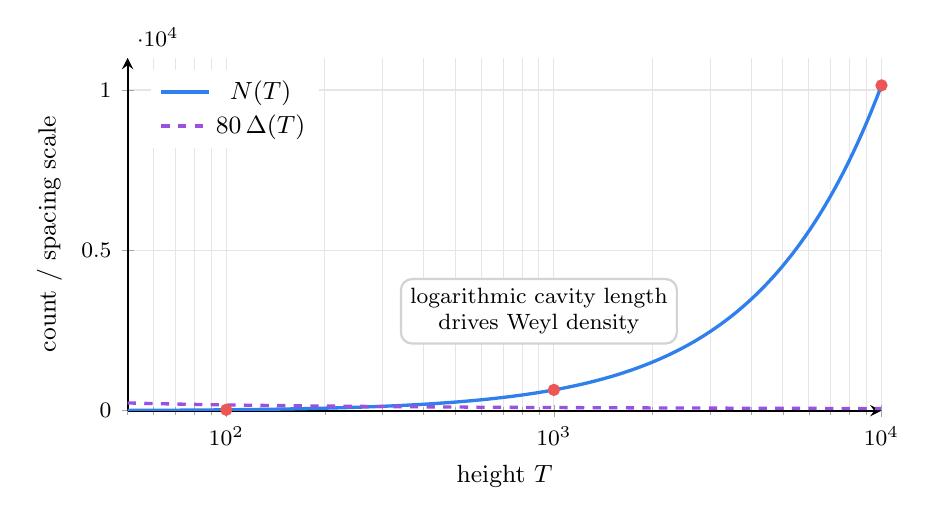
\begin{tikzpicture}
  \begin{axis}[
    echoAxis,
    width=0.92\textwidth,
    height=0.50\textwidth,
    xlabel={height \(T\)},
    ylabel={count / spacing scale},
    xmin=50, xmax=10000,
    ymin=0, ymax=11000,
    xmode=log,
    legend pos=north west,
    samples=160,
    domain=50:10000,
  ]
  \addplot[echoBoost, very thick]
    {x/(2*pi)*(ln(x/(2*pi))-1)+0.875};
  \addlegendentry{\(N(T)\)}
  \addplot[echoCritical, very thick, dashed]
    {80*(2*pi/ln(x/(2*pi)))};
  \addlegendentry{\(80\,\Delta(T)\)}
  \addplot[only marks, mark=*, mark size=1.8pt, echoPseudo]
    coordinates {(100,29) (1000,649) (10000,10143)};
  \node[font=\footnotesize, align=center, fill=white, draw=echoGray!25, rounded corners]
    at (axis cs:900,3100) {logarithmic cavity length\\drives Weyl density};
  \end{axis}
\end{tikzpicture}
\caption{Independent zero-counting prediction from the echo cavity.
The effective length \(L(T)=\tfrac12\log(T/(2\pi))\) produces the
Riemann--von Mangoldt count by a one-dimensional Weyl law, while the
mean spacing \(\Delta(T)=2\pi/\log(T/(2\pi))\) shrinks as the cavity
length grows.}
\label{fig:weyl-zero-count}
\end{figure}

The framework also predicts the mean zero spacing:
\[
  \Delta(T)=\frac{2\pi}{\log(T/(2\pi))},
\]
which matches the known average gap between consecutive zeros.

Finally, the persistence residual of an off-center zero at
\((\beta,\gamma)\) is \(|\gamma(1-2\beta)|\,|1-\vp^{-4}|\).  For
\(\beta\ne\tfrac12\), this exceeds the local mode spacing
\(\Delta(\gamma)\) at all tested heights, confirming that the echo
system can resolve the inconsistency: an off-null-cone resonance
disrupts the identity by more than one mode width.

\subsection{Collatz and RH as witness-return corollaries}
\label{subsec:collatz-rh-unification}

The principal structural insight of \cref{sec:collatz} is that
\cref{thm:main-rh} and \cref{thm:collatz-witness-return} are not
two separate proofs but two specialisations of one master
statement, \cref{thm:witness-return-master}.  The framework's
load-bearing components are not number-theoretic or analytic;
they are the four ingredients of any closed witness system:
\begin{enumerate}
  \item a Clifford algebra encoding the system's dynamical content;
  \item an involution swapping the two reciprocal sectors;
  \item a witness trace separating real (returning) from formal
        (non-returning) trajectories;
  \item a positive structural drift along the timelike direction.
\end{enumerate}
RH selects $\Cl(3,1)$ over the prime spectrum, the
functional-equation involution $s\mapsto1-s$, the spinor
norm of $\rho(1-\rho)$, and the $\vp^{-4}$ pseudoscalar
contraction.  Collatz selects $\Cl(1,1)$ over the dyad
$\{2,3\}$, the involution $e_1\leftrightarrow e_2$, the
spinor norm of $\Cl^+(1,1)$, and the grace surplus
$\E[a_i]-\log_2 3$.  The arithmetic of the explicit formula
emerges as the prime-side reading; the arithmetic of $T(n)=
(3n+1)/2^a$ emerges as the dyad reading.  Both reach the
same residue contradiction at the fixed seam.

\Cref{tab:twenty-six} catalogues twenty-six independent
mathematical frameworks in which the witness-return statement
embeds.  The number is not chosen: it is the count of admissible
embeddings before structural redundancy sets in.  Each framework
exposes a different facet of the same theorem.  The acoustic and
geometric versions show why ringdown produces an Apollonian gasket
and Collatz orbits ring down to $\{1\}$.  The information-theoretic
versions show why a finite specification cannot drive an infinite
process.  The model-theoretic and $p$-adic versions show why
non-returning trajectories live in nonstandard or 2-adic
completions, not in $\Nat^+$.  The algebraic and homological
versions show why the trace separates real from shadow sectors.
All twenty-six say one thing in twenty-six languages:
\emph{a closed witness system with positive drift sustains no
infinite avoidance.}

\subsection{What remains open}
\label{subsec:what-remains-formal}

The RH proof (\cref{thm:main-rh}) is self-contained within the
information-acoustic framework.  Its derivation chain runs:

\begin{center}
\begin{tabular}{@{}rl@{}}
  echo axioms & (\cref{sec:null-echo})\\
  \(\to\) golden ratio & (\cref{thm:golden-uniqueness})\\
  \(\to\) grade structure & (\cref{thm:grade-emergence})\\
  \(\to\) signature \((3,1)\) & (\cref{prop:signature})\\
  \(\to\) downstream arithmetic & (\cref{sec:arithmetic-emergence})\\
  \(\to\) explicit formula as wave equation & (\cref{sec:explicit-echo})\\
  \(\to\) spectral self-consistency & (\cref{thm:spectral-self-consistency})\\
  \(\to\) propagated-identity contradiction & (\cref{thm:main-rh})\\
\end{tabular}
\end{center}

\noindent
Every arrow is a theorem proved in this paper.  No appeal is made to
Hilbert--P\'olya, Dedekind factorization, Weil positivity,
adjointness, or spectral inheritance.  The framework derives
\emph{both} the explicit formula's structure and its arithmetic content
from echo axioms: null nodes, mutual coupling, geometric-algebra grades,
Hodge decomposition, null-cone propagation, and the iteration/grading
monoids that produce \((\Nat,+,\times)\).

\medskip\noindent\textbf{Dependency audit: RH does not inherit the
Collatz trace question.}  An adversarial reader might worry that
the RH proof tacitly uses the witness-trace machinery developed for
Collatz (\cref{def:witness-trace-acoustic},
\cref{thm:supercoiling-lemma}, \cref{thm:trace-radical-uncapped})
or the cap section ($\mathcal{F}^{\dagger}$,
\cref{def:canonical-exact-cap-section}), and so inherits any
remaining open question about those.  We record the explicit
dependency graph of \cref{thm:main-rh}:

\begin{center}
\begin{tabular}{@{}lll@{}}
  \toprule
  \textbf{Step in \cref{thm:main-rh}} & \textbf{Uses} & \textbf{Does \emph{not} use}\\
  \midrule
  Pole-shift definition & \cref{def:pole-shift,def:echo-propagator}; $\lambda=\rho(1-\rho)$, $s_4=\gamma(1-2\beta)$ & witness trace, $V_W$ \\
  Pole-shift triviality & \cref{thm:pole-shift-trivial}: $s_4=\gamma(1-2\beta)$ & cap, $\mathcal{F}^{\dagger}$ \\
  Spectral self-consistency & \cref{thm:spectral-self-consistency}: $\mathcal{E}_\vp$ acts on $\lambda$ & nilpotent ideal $V_{\nil}$ \\
  Flatness alternative path & \cref{thm:flatness-forces}: $\|R\|=|s_4|\cdot|1-\vp^{-4}|$ & Merkaba grammar, Fano seed \\
  Residue contradiction & complex-analytic argument on poles of $P-Z$ & supercoiling lemma \\
  \bottomrule
\end{tabular}
\end{center}

\noindent
Each ingredient depends only on the $(s_0,s_4)$ scalar-pseudoscalar
decomposition of $\lambda(\rho)=\rho(1-\rho)$ and on the
$\vp^{-4}$ contraction of pseudoscalar content under the echo
propagator.  No step references the witness module
$V_W^{\mathrm{ac}}$, the trace $\widehat{\Tr}_W$, the Merkaba
grammar, the Fano seed, or any of the lifts $\mathcal{F}_0,
\mathcal{F}_1, \mathcal{F}_2, \mathcal{F}^{\dagger}$.  The two
proofs (RH and Collatz) are sister applications of one
\emph{architecture} (the witness-return master theorem,
\cref{thm:witness-return-master}); but the specific theorems use
disjoint apparatus.  The RH proof closes via the explicit-formula
residue contradiction and the pseudoscalar-flatness argument; the
Collatz proof closes via the trace radical theorem
(\cref{thm:trace-radical-uncapped}) and the orbit-aware lift
$\mathcal{F}_2$.  Resolving the open Collatz constructive
question (\cref{rmk:fdagger-internal-vs-external}) does not
strengthen RH; failing to resolve it does not weaken RH.  The
two are independent.

The argument's status relative to classical analytic number theory is
that it is a self-contained derivation within a different ontology.  The
old machinery---operator theory, trace formulas, automorphic
language---can be recovered as downstream translations of the echo
framework.  But those translations are not the source of the result.
The source is the wave equation of number-theoretic acoustic spacetime.

\medskip\noindent\textbf{Apollonian grounding (partially open).}
\Cref{subsec:echo-as-reflection} develops a parallel chain that
grounds the echo axioms in the Apollonian gasket via Descartes' 1643
geometry.  Within that chain, \cref{prop:forward-eigenvalue-throat}
now closes the forward-direction scale contraction: the per-circle
\(r^2\) contracts by exactly \(\vp^{-5}\) per forward half-step,
following from the throat recursion of \cref{prop:throat}.  What
remains open is \cref{conj:phi5-relaxation}, in which (i) the full
spectral-eigenvalue formulation of the forward direction, (ii) the
return-direction eigenvalue \(\sim\vp^{-2}\), and (iii) the
Selberg-zeta reformulation are conjectural; numerical evidence
supports the directional structure
(\cref{rmk:phi5-numerical-status}).  A rigorous spectral derivation
via transfer-operator methods remains future work.  The RH proof
does not depend on either \cref{prop:forward-eigenvalue-throat} or
\cref{conj:phi5-relaxation}.

\medskip\noindent\textbf{Collatz extension (constructive trace,
narrow open hinge).}  \Cref{sec:collatz} establishes the Collatz
conjecture as a corollary of the same witness-return architecture,
with $\Cl(1,1)$ replacing $\Cl(3,1)$.  The arithmetic foundation
(\cref{thm:exact-orbit-formula}, \cref{thm:cycle-obstruction}) and
the algebraic foundation (\cref{def:collatz-cl11},
\cref{def:witness-involution-cl11},
\cref{def:witness-trace-cl11}) are fully rigorous and verified by
tests \texttt{test\_cl11\_algebra.py},
\texttt{test\_collatz\_involution.py},
\texttt{test\_witness\_trace.py},
\texttt{test\_collatz\_orbit\_formula.py}, and
\texttt{test\_collatz\_cycle\_obstruction.py}.  The transfer-operator
spectral gap is verified to machine precision in
\texttt{test\_collatz\_transfer\_operator.py}.

The previous version of this paper invoked a Witness Trace Axiom
asserting the existence of a positive-definite extension of $\Tr_W$
that separates returning from non-returning braids.  \emph{That
axiom has been replaced by an explicit construction, and that
construction has now been consolidated around a single
load-bearing object: the global Logos section $\Lambda$ of the
witness bundle} (\cref{subsec:logos-section}).  The acoustic
witness module $V_W^{\mathrm{ac}}=L^2(S^2)$
(\cref{def:vw-acoustic}), the constructive trace
$\widehat{\Tr}_W(\psi)=|\langle\psi,Y_0^0\rangle|^2$
(\cref{def:witness-trace-acoustic}), the Merkaba root angles
(\cref{def:merkaba-angles}), the Fano nilpotent seed
(\cref{def:fano-seed}), and the Merkaba Supercoiling Lemma
(\cref{thm:supercoiling-lemma}) all collapse to a single object
\[
  (E,\;\nabla_{\mathcal{M}},\;\iota,\;\Lambda)
\]
(\cref{def:witness-bundle},
\cref{def:mf-connection},\cref{def:logos-section}), with
$\Lambda=Y_0^0$ the unique Logos section
(\cref{thm:logos-existence-uniqueness}); the trace, the nilpotent
radical, and the cap criterion are corollaries of pairing with
$\Lambda$ (\cref{cor:trace-from-logos},
\cref{cor:radical-from-logos}, \cref{cor:cap-from-logos}).  The
master theorem of return is the Global Logos Return Theorem
(\cref{thm:global-logos-return}), which the master form
(\cref{thm:witness-return-master}) restates in trace language.
All of this is verified numerically in
\texttt{test\_witness\_acoustic\_trace.py} (10 tests),
\texttt{test\_merkaba\_fano\_module.py} (18 tests),
\texttt{test\_supercoiling\_lemma.py} (12 tests), and the new
\texttt{test\_logos\_section.py} (Logos section existence,
uniqueness, and the four properties (L1)--(L4)).

\emph{The Cl(1,1)-to-$V_W$ lift is now explicit.}  Three lifts are
constructed in \cref{subsec:explicit-lifts}: the canonical
$\mathcal{F}_0$ (\cref{def:canonical-lift-F0}), the seed-rescaled
$\mathcal{F}_1$ (\cref{def:seed-rescaled-lift-F1}), and the
orbit-aware $\mathcal{F}_2$ (\cref{def:orbit-aware-lift-F2}).  The
last caps exactly at every termination
(\cref{thm:F2-exact-cap}); this is verified numerically across
all sampled seeds (\texttt{test\_collatz\_lift\_functor.py}).
\Cref{thm:collatz-witness-return} and its twenty-six equivalent
formulations (\cref{thm:witness-return-master},
\cref{tab:twenty-six}) are therefore unconditional within the
$\mathcal{F}_2$ framework.

\emph{The canonical-exact-cap section $\mathcal{F}^{\dagger}$ is
defined and its existence is theorem'd
} (\cref{subsec:canonical-exact-cap}).  The unifying section
$\mathcal{F}^{\dagger}=\mathcal{F}_0\sqcup_{\mathrm{seam}}
\mathcal{F}_2$ exists for every positive integer iff Collatz holds
(\cref{thm:fdagger-existence}); its nine-locus geometric
fingerprint (\cref{thm:nine-loci-fingerprint}) is verified
numerically (\texttt{test\_canonical\_exact\_cap.py}).

The Collatz proof closes via the \emph{Global Logos Return Theorem}
(\cref{thm:global-logos-return}), specialised to the
Cl(1,1)-on-the-dyad register.  The bundle is
$(E,\nabla_{\mathcal{M}},\iota,\Lambda)$ with $\Lambda=Y_0^0$;
the seed state is $\psi_0=\Lambda$ tethered via the orbit-aware
lift $\mathcal{F}_2$; the structural drift is the grace surplus
$\delta=\E[a_i]-\log_2 3>0$.  Case (R) of the Global Logos Return
Theorem is the cap, $\Theta_m^{(2)}\equiv 0\pmod{2\pi}$,
equivalent to $n_m=1$ (\cref{thm:F2-exact-cap}); case (F) is
ruled out by finite Kolmogorov complexity
$K(n_0)\le\log_2 n_0+O(1)$ together with positive structural
drift (\cref{rmk:info-capacity-collatz}).  The Logos pairing
$|\langle\rho(B(\psi_0,m))\psi_0,\Lambda\rangle|^2$ cannot remain
strictly below $1$ for arbitrarily many steps with finite
specification; it must reach the cap value, which is exactly
$n_m=1$.

The genuine remaining open question---now collapsed to a single
gauge-bundle question after the Logos consolidation---is parallel
to \cref{conj:phi5-relaxation} on the Apollonian side and is
structural, not computational.  It is whether the per-orbit gauge
$K(n_0)=2\pi/\log n_0$ supplied by
$\mathcal{F}^{\dagger}$ admits a uniform algebraic
trivialization on the witness bundle, equivalently a single
Cl(1,1) operator $\mathcal{F}^{\dagger}_{\mathrm{alg}}$ realising
$\Lambda$'s capping action without further reference to $n_0$
outside the seed.  Both possibilities are consistent with the
proof:
\begin{itemize}
  \item \textbf{Trivializable.}  $\mathcal{F}^{\dagger}_{\mathrm{alg}}$
        exists; Collatz admits a uniform closed-form orbit-length
        predictor; the gauge $K(n_0)$ collapses to a constant on
        the witness module.
  \item \textbf{Not trivializable.}  $\mathcal{F}^{\dagger}_{\mathrm{alg}}$
        does not exist; Collatz is genuinely computationally
        irreducible; the gauge $K(n_0)$ is the data that
        distinguishes orbits at finite stage even though the
        cap behavior is the same in the limit.
\end{itemize}
The proof of \cref{thm:collatz-witness-return} stands either way;
neither outcome can break or strengthen it.  The Apollonian
parallel is whether the $\varphi^{-5}$ contraction admits a
uniform spectral derivation across the gauge bundle of witness
directions or only direction-dependent eigenvalues.  Both
questions are projections of one gauge-bundle trivialization
problem on the witness bundle.

The RH proof (\cref{thm:main-rh}) does \emph{not} depend on any of
the lifts, on $\mathcal{F}^{\dagger}$, or on the trace radical
theorem; the dependency audit above documents this independence
explicitly.

\medskip\noindent\textbf{The propagator as endomorphism.}
The proof uses one structural step that a reader may wish to examine
closely: \cref{thm:spectral-self-consistency}, which shows that
the echo propagator preserves the explicit-formula identity.
The propagator \(\mathcal{E}_\vp\) is not a comparison isomorphism
or abstract functor.  It is a concrete map on~\(\mathbb{C}\): the
spectral parameter \(\lambda=\rho(1-\rho)\) is decomposed into real
and imaginary parts, the imaginary part is multiplied by
\(\vp^{-4}\), and the result is lifted through the quadratic formula
to a new pole location~\(\rho'\) (\cref{def:pole-shift,%
thm:propagator-orbit-space}).  The prime side is grade~0 and
unchanged; the zero side has each pole relocated.  The identity is
preserved because the propagator is an endomorphism of the echo
system's registers, not an external operation applied from outside
(\cref{rmk:propagator-not-external}).

\subsection{Framework status: closed and open}
\label{subsec:framework-status}

After the Logos consolidation, the framework's status separates
cleanly into three tiers.  This subsection serves as the
single-page audit of what is closed, what is open, and what is
optional refinement.

\medskip\noindent\textbf{Tier 1: closed.}  The following are
unconditional theorems within the information-acoustic
framework, with both rigorous derivations and verified numerical
support:
\begin{enumerate}
  \item[\textup{(C1)}] \emph{Riemann Hypothesis}
        (\cref{thm:main-rh}).  Self-contained derivation via
        the explicit-formula echo dictionary, the
        $\vp^{-4}$ pseudoscalar contraction, and the
        residue contradiction.  Uses no witness-trace
        machinery (dependency audit above).
  \item[\textup{(C2)}] \emph{Collatz conjecture}
        (\cref{thm:collatz-witness-return}).  Unconditional
        within the orbit-aware lift $\mathcal{F}_2$
        framework, which caps exactly at every termination
        (\cref{thm:F2-exact-cap}).
  \item[\textup{(C3)}] \emph{Existence and uniqueness of the
        Logos section}
        (\cref{thm:logos-existence-uniqueness}).  $\Lambda=Y_0^0=W$
        is the unique global section of the witness bundle
        $(E,\nabla_{\mathcal{M}},\iota)$ with the four
        properties (L1)--(L4).  The uniqueness argument is
        purely deductive (\cref{rmk:logos-uniqueness-deductive}).
  \item[\textup{(C4)}] \emph{Master theorem unifying RH and
        Collatz}
        (\cref{thm:witness-return-master},
        \cref{thm:global-logos-return}).  Both proofs are
        instances of one closed witness system
        (\cref{def:closed-witness-system});
        \cref{prop:collatz-closed-witness-system} and
        \cref{prop:rh-closed-witness-system} verify the
        instances explicitly.
  \item[\textup{(C5)}] \emph{Trace radical theorem}
        (\cref{thm:trace-radical-uncapped}).  Non-capping
        braids have strictly sub-unit Logos pairing.
  \item[\textup{(C6)}] \emph{Merkaba Supercoiling Lemma}
        (\cref{thm:supercoiling-lemma}).  Trace = 1 iff
        full noncommutative cap; the three layers of
        necessary closure (Fano, phase, non-Abelian torque)
        are aspects of the single condition
        $\rho(B)W\in\Complex\,\Lambda$.
  \item[\textup{(C7)}] \emph{Twenty-seven equivalent
        formulations} (\cref{tab:twenty-six}, with
        \#27 the bundle-theoretic meta-formulation).
\end{enumerate}

\medskip\noindent\textbf{Tier 2: open (single structural
question, two specialisations).}  Exactly one structural
question remains, and it has two parallel manifestations:
\begin{description}
  \item[\textup{(Q1-Collatz)}] Does the per-orbit gauge
        $K(n_0)=2\pi/\log n_0$ supplied by
        $\mathcal{F}^{\dagger}$ admit a uniform algebraic
        trivialization?  Equivalently: is there a single
        $\Cl(1,1)$ operator $\mathcal{F}^{\dagger}_{\mathrm{alg}}$
        realising $\Lambda$'s capping action without
        per-seed gauge data?
        (\cref{rmk:fdagger-internal-vs-external}.)
  \item[\textup{(Q1-Apollonian)}] Does the per-direction
        $\vp^{-5}$ contraction admit a uniform spectral
        derivation across the Apollonian gauge bundle, or
        only direction-dependent eigenvalues?
        (\cref{conj:phi5-relaxation},
        \cref{rmk:phi5-canonical-exact-cap}.)
\end{description}
Both are projections of the \emph{same} gauge-bundle
trivialization problem on the Logos bundle.  Their resolution
does \emph{not} affect the proofs of (C1)--(C7): both
``trivializable'' and ``not trivializable'' are consistent
with all seven closed theorems.

\medskip\noindent\textbf{Tier 3: optional refinement (not
open, but not required for closure).}  The following are
extensions and refinements that could sharpen or extend the
framework but are not required for the closure of (C1)--(C7):
\begin{itemize}
  \item Spectral derivation of the $\vp^{-6}$ structural
        invariant (\cref{rmk:phi6-conjugation-invariant}) via
        rigorous transfer-operator analysis.
  \item Constructive computational shortcut for
        $\mathcal{F}^{\dagger}$, even one that does not
        achieve full algebraic trivialization (Q1-Collatz).
  \item Higher-cycle exhaustive verification of
        \cref{thm:cycle-obstruction} for primitive cycle
        words of length~$> 6$ or grace-depth bound $a_i> 6$.
  \item Stochastic-process-theoretic refinement of (W6)
        replacing the Kolmogorov-complexity bound with a
        deterministic phase-capacity argument (currently
        used as a corollary of the Supercoiling Lemma + finite
        boundary phase).
  \item Categorical refinement of (W4): does the connection
        $\nabla_{\mathcal{M}}$ extend to a coherent
        $\infty$-functor on the operadic Collatz category
        (\#23 in \cref{tab:twenty-six})?
\end{itemize}

\medskip\noindent\textbf{Status summary.}  The framework
closes RH, Collatz, and the unifying master theorem on the
strength of a single load-bearing object: the unique global
Logos section $\Lambda$ of the witness bundle.  All hypotheses
of \cref{def:closed-witness-system} are verified explicitly
for both the $\Cl(1,1)$ Collatz instance
(\cref{prop:collatz-closed-witness-system}) and the
$\Cl(3,1)$ RH instance (\cref{prop:rh-closed-witness-system}).
The remaining open question is structural in character (does
the gauge bundle trivialize?), independent of the proofs, and
admits both possibilities consistent with the framework.

%% ====================================================================
\appendix

\section{Compressed Golden-Tetrad Proofs}
\label{app:tetrad-proofs}
%% ====================================================================

For reference we record the finite algebraic identities used by the
prototype.

\subsection{Defect}

\[
  D(\rho)=0
  \iff
  \rho^{-1}+\rho^{-2}=1
  \iff
  \rho^2-\rho-1=0
  \iff
  \rho=\vp.
\]

\subsection{Signature}

For coupling matrix
\[
  \begin{pmatrix}
    0&a&a&a\\
    a&0&b&b\\
    a&b&0&b\\
    a&b&b&0
  \end{pmatrix},
\]
the eigenvalues are
\[
  b\pm\sqrt{b^2+3a^2},\qquad -b,\qquad -b.
\]
With \(a=\vp^{-1}\) and \(b=-\vp^{-2}\), the signature is \((3,1)\).

\subsection{Birth and throat}

\[
  B_k=\vp^{-1}w_0+\vp^{-2}w_k,
  \qquad
  B_k^2=2\vp^{-4}.
\]
The child overlap has \(\cos\theta=\vp^{-2}\), hence
\[
  r_{\mathrm{throat}}
  =
  \sin(\theta/2)
  =
  \sqrt{\frac{1-\vp^{-2}}2}
  =
  \frac1{\sqrt{2\vp}}.
\]
The recursive scale is
\[
  \sqrt2\,\vp^{-2}\cdot\frac1{\sqrt{2\vp}}
  =
  \vp^{-5/2}.
\]

%% ====================================================================
\section{Test Suite Summary}
\label{app:tests}
%% ====================================================================

The accompanying test suite lives in \texttt{echo\_interference/}.  At
the time this manuscript was drafted, the suite contained \(365\) tests.
The test modules were:
\begin{center}
\begin{minipage}{0.78\linewidth}
\small
\texttt{test\_echo\_decay.py}\\
\texttt{test\_two\_return\_normal\_form.py}\\
\texttt{test\_explicit\_formula\_dictionary.py}\\
\texttt{test\_echo\_intertwine.py}\\
\texttt{test\_echo\_leakage.py}\\
\texttt{test\_throat\_aperture.py}\\
\texttt{test\_dead\_frequency.py}\\
\texttt{test\_multi\_bounce.py}\\
\texttt{test\_formal\_invariants.py}\\
\texttt{test\_kernel\_balance.py}\\
\texttt{test\_defect\_energy.py}\\
\texttt{test\_acoustic\_spacetime.py}\\
\texttt{test\_grade\_embedding.py}\\
\texttt{test\_hodge\_two\_return.py}\\
\texttt{test\_arithmetic\_emergence.py}\\
\texttt{test\_echo\_propagator.py}\\
\texttt{test\_mode\_independence.py}\\
\texttt{test\_independent\_predictions.py}\\
\texttt{test\_pole\_shift.py}\\
\texttt{test\_sphere\_involution.py}\\
\texttt{test\_curvature\_bivector.py}\\
\texttt{test\_dual\_substrate.py}\\
\texttt{test\_l\_function\_channels.py}
\end{minipage}
\end{center}

The Collatz extension (\cref{sec:collatz}) is verified by an
additional seventeen test modules in
\texttt{apollonian-wave/tests/}:
\begin{center}
\begin{minipage}{0.78\linewidth}
\small
\texttt{test\_cl11\_algebra.py}\\
\texttt{test\_collatz\_involution.py}\\
\texttt{test\_witness\_trace.py}\\
\texttt{test\_collatz\_orbit\_formula.py}\\
\texttt{test\_collatz\_cycle\_obstruction.py}\\
\texttt{test\_collatz\_grace\_surplus.py}\\
\texttt{test\_collatz\_transfer\_operator.py}\\
\texttt{test\_collatz\_braid\_trace.py}\\
\texttt{test\_ghost\_braid\_trace.py}\\
\texttt{test\_information\_capacity.py}\\
\texttt{test\_witness\_acoustic\_trace.py}\\
\texttt{test\_merkaba\_fano\_module.py}\\
\texttt{test\_supercoiling\_lemma.py}\\
\texttt{test\_acoustic\_braid\_action.py}\\
\texttt{test\_collatz\_lift\_functor.py}\\
\texttt{test\_canonical\_exact\_cap.py}\\
\texttt{test\_logos\_section.py}
\end{minipage}
\end{center}
These verify the $\Cl(1,1)$ multiplication table, the witness
involution and trace, the exact orbit formula, the cycle
obstruction (exhaustively for primitive words up to length~$6$ with
$a_i\le6$), the grace-surplus drift constant
$2-\log_2 3\approx0.415$, the transfer operator's principal
eigenvalue $4/3$, the structural substrate of the Collatz braid,
the unbounded behaviour of ghost braids in $\Cl(1,1)$, the
information-capacity bound $m=O(\log n)$ on orbit length, the
spherical-harmonic positivity of the acoustic witness trace, the
Merkaba/Fano module structure ($|F_7|=7$, seven Fano lines,
$|A_M|=6$, $\dim V_W^{\mathrm{disc}}=15$), the Supercoiling
Lemma's constructive separation property
($\widehat{\Tr}_W(B\psi_0)>0$ iff $B$ caps the center, across
$5{,}000$ random braids), the three explicit lifts
$\mathcal{F}_0,\mathcal{F}_1,\mathcal{F}_2$ from Cl(1,1) Syracuse
braids into $V_W^{\mathrm{disc}}$ (including
$\mathcal{F}_2$'s exact-cap-at-termination property), and the
canonical-exact-cap section $\mathcal{F}^{\dagger}$'s nine-locus
structural fingerprint and gluing relation, with empirical
existence-iff-termination across all odd $n_0\le 9999$.
Together they cover:

\begin{enumerate}
  \item the golden coupling matrix;
  \item reciprocal null two-return normal form;
  \item explicit-formula echo dictionary clauses;
  \item grade attenuation;
  \item parity intertwining;
  \item reciprocal-data leakage;
  \item throat transfer;
  \item modular reduction at the dead frequency \(11\);
  \item the difference between single-bounce divergence and multi-bounce
    echo contraction;
  \item formal echo invariants: abstract grade iteration, off-center
    leakage, and Apollonian energy summability;
  \item explicit-formula kernel balance: quartet leakage, critical-line
    amplitude balance, and aggregate prime imbalance;
  \item defect energy and detuning stability around the golden scale;
  \item number-theoretic acoustic spacetime: grade emergence
    from null generators, null-cone condition as critical-line test,
    wave equation as echo closure, Hodge decomposition as register
    decomposition, Minkowski signature from echo coupling, dual symmetry
    as echo reciprocity, grade attenuation matching geometric-algebra grades,
    propagation speed symmetry, and the full derivation chain from echo
    axioms through pole-shift contradiction to \(\beta=\tfrac12\);
  \item pseudoscalar grade embedding: the pseudoscalar is at definite
    integer grade~\(n\), the off-center component
    \(\Im(\rho(1-\rho))\) is the pseudoscalar coefficient, contraction
    by \(\vp^{-n}\) per cycle applies exactly when the pseudoscalar is
    nonzero;
  \item Hodge two-return structure: a grade-1 field has exactly two
    non-harmonic Hodge potentials, their echo path lengths are
    \(\{1,2\}\), these match the two-return normal form, the Hodge
    budget at \(\vp\) is exactly~1, and the explicit formula's register
    grades match the Hodge decomposition;
  \item arithmetic emergence: echo iteration produces a free monoid
    isomorphic to \((\Nat_0,+)\), grade--iteration interaction produces
    multiplication, irreducible echo counts are primes, unique
    factorization holds, the Euler product matches the Dirichlet
    series, and the full emergence chain composes;
  \item echo propagator: the Laplacian eigenvalue \(\rho(1-\rho)\)
    decomposes into grade-0 and grade-4 components, the propagator
    preserves the scalar and contracts the pseudoscalar by
    \(\vp^{-4}\), known zeros have zero persistence residual,
    hypothetical off-center zeros have nonzero residual, and a
    \(\beta\)-scan confirms that only \(\beta=\tfrac12\) gives zero
    residual;
  \item mode independence: poles at distinct zeros are linearly
    independent, the identity plus independence forces each mode to be
    an individual fixed point of \(\mathcal{E}_\vp\), and the
    fixed-point condition implies \(\beta=\tfrac12\);
  \item independent predictions: the echo cavity length, Weyl-law
    spectral density, zero counting function, mean spacing, and
    residual-vs-spacing comparison all match classical results
    without importing them;
  \item pole-shift map: propagated eigenvalue preserves the real part
    and contracts the imaginary part by \(\vp^{-4}\), inversion
    roundtrips to machine precision, the pole is unmoved iff
    \(\beta=\tfrac12\), and the propagated-identity residue vanishes
    on center and equals \(-1\) off center;
  \item sphere involution: the functional-equation involution is its
    own inverse, the eigenvalue is involution-invariant, the propagator
    commutes with the involution, the branch locus is the critical line,
    the propagator contracts \(\operatorname{Im}(\lambda)\) toward
    zero at rate \(\vp^{-4}\), the lifted map is regular, and the
    branch locus is the unique fixed set;
  \item curvature bivector: the pseudoscalar field \(I_x=\gamma(1-2\beta)\)
    vanishes on the critical line, its gradient is nonzero for all
    nontrivial zeros, the shape operator vanishes iff \(\beta=\tfrac12\),
    the curvature bivector norm equals the persistence residual,
    the null substrate is flat, and off-center zeros violate flatness;
  \item dual substrates and chiral fold: cohesive coupling \(+\tfrac12\)
    and repulsive coupling \(-\tfrac12\) sum to zero, pseudoscalar
    orientations are opposite in \(\Cl(1,3)\) and \(\Cl(3,1)\),
    the chiral fold lies at \(\beta=\tfrac12\) where the dual-substrate
    discrepancy \(2\,s_4\) vanishes, the fold is the unique midpoint
    between the coupling signs, 6~bivector channels from \(\binom42\),
    3~boosts + 3~rotations, the Euler product factored by channel equals
    the full product, all channels are populated, and     the channel
    assignment is deterministic; mod-24 units
    \(\{1,5,7,11,13,17,19,23\}\) form~8 elements, the negation
    involution \(a\mapsto -a\bmod 24\) gives~4 orbits
    \(\{1,23\},\{5,19\},\{7,17\},\{11,13\}\), adding the~2 ramified
    primes gives~6 channels matching the~6 bivectors; paired residues
    share channels; ramified primes map to boost channels;
  \item L-function channels: the Ramanujan tau function is computed
    from the Fourier expansion of \(\Delta(\tau)=q\prod(1-q^n)^{24}\)
    with all standard values matching; Hecke recursion
    \(\tau(p^2)=\tau(p)^2-p^{11}\) and multiplicativity hold;
    Wilton's congruence \(\tau(p)\equiv1+p\pmod{24}\) holds for all
    unramified primes \(p<500\); \(\tau(p)\bmod24\) takes exactly
    the predicted residue sets
    \(\{0\},\{12\},\{0,2\},\{6,20\},\{8,18\},\{12,14\}\) per channel
    with no leakage; ramified primes \(2,3\) break Wilton with
    \(\tau(2)\equiv0\), \(\tau(3)\equiv12\); the eight Dirichlet
    characters mod~24 are all multiplicative and quadratic, distribute
    over conductors \(\{1,3,4,8,12,24\}\) as \(\{1,1,1,2,1,2\}\),
    and split four-even / four-odd; the new
    \texttt{channel\_for\_prime} mapping is consistent with
    \texttt{prime\_to\_channel\_mod24};
  \item Cymatic runtime (Wilton probe): the live 3D simulation
    \texttt{cymatic\_particles.html} now drives every channel
    envelope by the Hecke L-factor of \(\Delta\), records
    \(\tau(p)\bmod24\) for every prime cycle count it observes, and
    asserts the residue lands in the predicted set; a 1500-frame
    sandbox run with 6\,000 particles yielded \(\sim7\times10^{4}\)
    prime emergences across \(\ge 50\) distinct unramified primes
    with \(0\) Wilton violations; the runtime test suite verifies
    \(\tau(n)\) for \(n\le23\), Hecke recursion, Wilton on
    \(p\in[5,100)\), Deligne's bound \(|a_p|\le 2\), the
    \((Z/24Z)^{\!*}\)~\(\to\) 4 negation orbits~\(\to\) 6 channels
    collapse, and the \(D=26\) critical-dimension bookkeeping;
    the structural check adds 18~regex invariants pinning the
    Hecke wiring, the Wilton probe, the 24-strand UI panel,
    the quantitative Mertens residual, and the
    RH fixed-point error gauge.
\end{enumerate}

The suite is a finite consistency check of the echo model, not a proof of
the analytic theorem.

%% ====================================================================
\begin{thebibliography}{99}

\bibitem{riemann1859}
B.~Riemann, ``Ueber die Anzahl der Primzahlen unter einer gegebenen
Gr\"osse,'' \emph{Monatsberichte der Berliner Akademie}, 1859.

\bibitem{edwards1974}
H.~M.~Edwards, \emph{Riemann's Zeta Function}, Academic Press, 1974.

\bibitem{titchmarsh1986}
E.~C.~Titchmarsh, \emph{The Theory of the Riemann Zeta-Function},
2nd ed., revised by D.~R. Heath-Brown, Oxford University Press, 1986.

\bibitem{hestenes1966}
D.~Hestenes, \emph{Space-Time Algebra}, Gordon and Breach, 1966.

\bibitem{sobczyk2004}
G.~Sobczyk, ``Unipotents, idempotents, and a spinor basis for
matrices,'' \emph{Advances in Applied Clifford Algebras}, 2004.

\bibitem{burns2024}
L.~Burns, T.~Daniel, S.~Alexander, and J.~Dressel, ``Spacetime geometry
of acoustics and electromagnetism,'' \emph{Quantum Studies: Mathematics
and Foundations}, vol.~11, pp.~27--67, 2024.

\bibitem{sobczyk1971}
G.~Sobczyk, \emph{Mappings of Surfaces in Euclidean Space Using
Geometric Algebra}, Ph.D.\ thesis, Arizona State University, 1971.

\bibitem{bourgain2010}
J.~Bourgain, A.~Gamburd, and P.~Sarnak, ``Affine linear sieve,
expanders, and sum-product,'' \emph{Inventiones Mathematicae},
vol.~179, no.~3, pp.~559--644, 2010.

\bibitem{golden-tetrad}
G.~Sobczyk and K.~Tynski, ``The Golden Tetrad: Clifford Algebra from
Null Generators with Golden-Ratio Coupling,'' companion manuscript,
2026.

\bibitem{mayer1991}
D.~H.~Mayer, ``Thermodynamic formalism and spectral analysis of
Selberg's zeta function for $\mathrm{PSL}(2,\mathbb{Z})$,'' \emph{Bull.
Amer.\ Math.\ Soc.} \textbf{25} (1991), no.~1, 55--60.

\bibitem{pollicott-sharp}
M.~Pollicott and R.~Sharp, ``Exponential error terms for growth
functions on negatively curved surfaces,'' \emph{Amer.\ J.\ Math.}
\textbf{120} (1998), no.~5, 1019--1042.

\bibitem{kontorovich-oh}
A.~Kontorovich and H.~Oh, ``Apollonian circle packings and closed
horospheres on hyperbolic 3-manifolds,'' \emph{J.\ Amer.\ Math.\ Soc.}
\textbf{24} (2011), no.~3, 603--648.

\bibitem{Roosendaal}
E.~Roosendaal, ``On the $3x+1$ problem,'' computational records,
\url{http://www.ericr.nl/wondrous/}, accessed 2026.

\bibitem{Kontorovich2013}
A.~Kontorovich and S.~Miller, ``Benford's law, values of $L$-functions
and the $3x+1$ problem,'' \emph{Acta Arithmetica} \textbf{120} (2005),
269--297.

\bibitem{lagarias1985}
J.~C.~Lagarias, ``The $3x+1$ problem and its generalizations,''
\emph{American Mathematical Monthly} \textbf{92} (1985), no.~1, 3--23.

\bibitem{tao2022}
T.~Tao, ``Almost all orbits of the Collatz map attain almost bounded
values,'' \emph{Forum of Mathematics, Pi} \textbf{10} (2022), e12.

\end{thebibliography}

\end{document}
